
%========= File containing the main LaTex document ========%
%                                                          %
% Copyright (C) ISI - All Rights Reserved                  %
% Proprietary                                              %
% Written by Med Hossam <med.hossam@gmail.com>, April 2016 %
%                                                          %
% @author: HEDHILI Med Houssemeddine                       %
% @linkedin: http://tn.linkedin.com/in/medhossam           %
%==========================================================%

%\documentclass[pfe]{./tpl/isipfe}
\documentclass[]{isipfe}
\graphicspath{{./img/}{./img/gen_fig/}}
\hfuzz=25pt

%\usepackage{hyperref}

\input{./tpl/new_commands}

% @author: Stoufa
% the command `\makeindex` is mandatory to create the index file main.idx
% https://tex.stackexchange.com/questions/9913/input-index-file-not-found
\makeindex
\begin{document}
    
%=== File containing Global Configuration of the report ===%
%                                                          %
% Copyright (C) ISI - All Rights Reserved                  %
% Proprietary                                              %
% Written by Med Hossam <med.hossam@gmail.com>, April 2016 %
%                                                          %
% @author: HEDHILI Med Houssemeddine                       %
% @linkedin: http://tn.linkedin.com/in/medhossam           %
%==========================================================%

%=========== You MUST type your information here ==========%
% global_config.tex file is designed to configure your     %
% cover pages (main, back and black covers)                %
%==========================================================%

%============= Config new columns type ==============%
\newcolumntype{L}{>{\raggedright\arraybackslash}}
\newcolumntype{R}{>{\raggedleft\arraybackslash}}
\newcolumntype{C}{>{\centering\arraybackslash}}
%==================================================%

%========= Config the cover section ==========%

\title{Design and Implementation of a Debugger with Instruction Trace Capabilities}

\author{Youssef HASNAOUI}
%%% if necessary
% Set isBinomal to true and type second author name
%\setboolean{isBinomal}{true}
%\secondAuthor{Prénom NOM}

\diplomaName{National Diploma in Infotronics Systems Engineering}
\speciality{Microelectronics \& Embedded Systems}
%\speciality{Génie des Télécommunications et Réseaux}
%\speciality{Génie Informatique des Systèmes Industriels}

%% Encadrant professionnel
\proFramerNameOne{Mohamed HAMROUNI}
\proFramerSpecialityOne{Application Engineer}

\academicFramerName{Faten Salem}
\academicFramerSpeciality{Professor}

%% Entreprise d'accueil
\companyName{STMicroelectronics}

%% Année universitaire
\collegeYear{2025 - 2026}

%%%%%% Signatures section %%%%%%

% You can simply remove theses sentences by typing an empty string
% \proSignSentence{}

\proSignSentence{J'autorise l'étudiant à faire le dépôt de son rapport de stage en vue d'une soutenance.}


%%% AR

%% To use latin characters inside the arabic text
% just put them inside the command \textLR{}
%%%%

%%% FR
\frenchAbstract{Ce rapport décrit un débogueur capable de capturer, de décoder et de présenter la trace d'instructions d'un microcontrôleur STM32. La trace d'instructions enregistre le chemin que le programme a réellement suivi dans son code. Le matériel qui la génère équipe une grande partie de la gamme STM32, mais il n'est exploitable qu'au moyen d'outils propriétaires et de sondes dont la plupart des développeurs ne disposent pas. Deux pilotes CoreSight ont été ajoutés à un serveur de débogage libre, afin que l'unité de trace et la mémoire tampon de trace intégrée au circuit puissent être configurées et vidées via la connexion de débogage habituelle. Une chaîne de traitement décode ensuite les octets capturés à l'aide de l'image du programme, reconstruit les instructions exécutées, rattache chacune à une fonction, à un fichier source et à une ligne, et présente le résultat au sein d'un environnement de développement, pendant une session de débogage. Une capture de 128 octets, extraite de la mémoire tampon intégrée au circuit et obtenue sans recourir aux broches de trace, permet de reconstruire 114 instructions exécutées.}
\frenchAbstractKeywords{Trace d'instructions, CoreSight, Embedded Trace Macrocell, Débogage embarqué, STM32, Debug Adapter Protocol, OpenOCD.}
%% dont go over 10 lines
%%% EN
\englishAbstract{This report describes a debugger that captures, decodes and presents the instruction trace of an STM32 microcontroller. Instruction trace records the path a program actually took through its code. The hardware producing it is present across much of the STM32 range, yet it is reachable only through proprietary tools and probes most developers do not have. Two CoreSight drivers were added to an open-source debug server, so that the trace unit and the on-chip trace buffer may be configured and drained over the ordinary debug connection. A pipeline decodes the captured bytes against the program image, reconstructs the executed instructions, attributes each to a function, a source file and a line, and presents the result inside a development tool during a live debug session. A capture of 128 bytes, drained from the on-chip buffer with no trace pins in use, reconstructs 114 executed instructions.}
\englishAbstractKeywords{Instruction trace, CoreSight, Embedded Trace Macrocell, Embedded debugging, STM32, Debug Adapter Protocol, OpenOCD.}
%% if you want to get rid of the company address just set the boolean variable to false
% PS : it's optional
\setboolean{wantToTypeCompanyAddress}{false}

\companyEmail{contact@company.com}
\companyTel{71 111 111}
\companyFax{71 222 222}
\companyAddressAR{نهج بحيرة ملاران - ضفاف البحيرة - تونس}
\companyAddressFR{Rue du Lac Malaren, Les Berges du Lac 1053 Tunis}

%============= Drafting placeholders ==============%
% Visible markers for artwork that is still to be produced.
% Grep for \needfig, \needtab or \needshot to find every outstanding item.
\newcommand{\needartwork}[3]{%
  \begin{center}
  \fbox{\parbox{0.92\linewidth}{%
    \textbf{[#1]}\\[2pt]
    \textit{Caption:} #2\\[2pt]
    \textit{Content:} #3}}
  \end{center}}
\newcommand{\needfig}[2]{\needartwork{FIGURE TO PRODUCE}{#1}{#2}}
\newcommand{\needtab}[2]{\needartwork{TABLE TO PRODUCE}{#1}{#2}}
\newcommand{\needshot}[2]{\needartwork{SCREENSHOT TO CAPTURE}{#1}{#2}}
% Outstanding work on the text itself, as opposed to missing artwork.
\newcommand{\needwork}[1]{%
  \begin{center}
  \fbox{\parbox{0.92\linewidth}{\textbf{[TODO]}\\[2pt] #1}}
  \end{center}}
%==================================================%

%============= Chapter cross-references ==============%
% The class calls \minitoc from inside \@makechapterhead, which leaves
% \@currentlabel holding the number of the preceding section. A \label placed
% after \chapter therefore records that section number instead of the chapter
% number. \chaplabel sets \@currentlabel to the chapter number first.
% isipfe.cls calls \makeatletter and never restores the catcode, and
% tpl/cover_page.tex relies on that, so the previous state is saved and
% restored here rather than forcing \makeatother.
\expandafter\edef\csname restore@at@code\endcsname{%
  \catcode`\noexpand\@=\the\catcode`\@\relax}
\makeatletter
\newcommand{\chaplabel}[1]{%
  \protected@edef\@currentlabel{\thechapter}%
  \label{#1}}
\csname restore@at@code\endcsname
%==================================================%


    \frontmatter
        \thispagestyle{cover}%
\newgeometry{bottom=25mm,left=20mm,top=15mm,right=20mm}
\hspace{-47pt}
\begin{minipage}[l]{0.2\columnwidth}
    \vspace{6mm}
    
\includegraphics[width=1.1\columnwidth]{img/ST_Summer_Internship/logo_enicar.jpg}\\
\end{minipage}
\hfill
\begin{minipage}[l]{0.6\columnwidth}
    \centering
    \footnotesize
    \textbf{{Republic of Tunisia}}\\
    \vspace{1.5mm}
    \textbf{{Ministry of Higher Education\\
                and Scientific Research}}\\
    \vspace{1.5mm}
    \textbf{{University of Carthage }}\\
    \vspace{1.5mm}
    \textbf{{National Engineering School of Carthage}}
\end{minipage}
\hfill
\begin{minipage}[l]{0.02\columnwidth}
\end{minipage}
\hfill
\begin{minipage}[l]{0.18\columnwidth}
    \vspace{6mm}
    
\includegraphics[width=1.1\columnwidth]{img/ST_Summer_Internship/uni_car.png}\\
\end{minipage}
\vskip1.5cm

\begin{center}
    {\LARGE{\textbf{\textsc{End of Studies Project Report}}}}\\
    \vskip0.5cm
    \large

\end{center}

\begin{center}
    \textrm{By}\\
    \vskip0.3cm
    {\ifthenelse{\boolean{isBinomal}}
    {% IF TRUE
        \begin{center}
            \large\textbf{\@author}~~~~~ et ~~~~~
            \large\textbf{\@secondAuthor}
        \end{center}
    }
    {\Large\textbf{\@author}}% FALSE
    }
    \vskip12mm

    \definecolor{isiBlue}{RGB}{31, 78, 121}

    \begin{changemargin}{-9mm}{0cm}
        \begin{minipage}[l]{1.1\columnwidth}
            \begin{tcolorbox}[colframe=black,colback=white,boxrule=0pt,toprule=3pt,bottomrule=3pt,arc=0pt,top=0mm,right=0mm,left=0mm,bottom=0mm,boxsep=0.5mm]{
                    \begin{tcolorbox}[colframe=black,colback=white, boxrule=0pt,toprule=1pt,bottomrule=1pt,arc=0pt,enlarge bottom by=-0.9mm, auto outer arc]
                        \centering
                        {\huge\textbf{\@title }}
                    \end{tcolorbox}
                }
            \end{tcolorbox}
        \end{minipage}
    \end{changemargin}

\end{center}
\vskip8mm%

\begin{center}
    \large
    \begin{minipage}[c]{0.28\columnwidth}
        Professional Supervisor:
        \newline
        Academic Supervisor:
    \end{minipage}
    \hfill
    \begin{minipage}[c]{0.42\columnwidth}
        \textbf{\@proFramerNameOne}\\
        \textbf{\@academicFramerName}
    \end{minipage}
    \hfill

\end{center}
\vskip16mm

\begin{center}
    \large
    Project Elaborated Within \@companyName\\
    \vskip0.2cm

    \begin{figure}[h]
        \centering
        {\color{black}{\fboxrule=2.5pt\fbox{
\includegraphics[width=0.43\columnwidth]{img/ST_logo_2024_blue.jpg}}}}
    \end{figure}
\end{center}
\afterpage{\blankpage}

        %\include{tpl/cover_page_black}
        %\input{tpl/signatures}

        \setcounter{page}{0}
        \input{dedicaces}
        \thispagestyle{frontmatter}
        \chapter*{\huge Acknowledgements}

\begin{center}
    \it \LARGE
    I would like to sincerely thank everyone who had a hand in the development of this project.

    Firstly, I want to express my utmost appreciation to \textbf{Mohamed HAMROUNI}, his guidance and support has been invaluable, and has kept me motivated and determined to give my best effort.

    I would also like to thank my professor \textbf{Faten SALEM} for providing the essential foundation to pursue this domain of expertise and for her captivating curiosity, which insipred me to continuously expand the boundaries of my knowledge.

    Last but not least, to every single person that contributed to the successful completion of this project with their constant support and motivation, you have my utmost thanks.
\end{center}

        \thispagestyle{frontmatter}

        \setcounter{secnumdepth}{3}
        \setcounter{tocdepth}{2}
        \tableofcontents
        \thispagestyle{frontmatter}
        %uncomment from here ----
        \clearpage
        \phantomsection
        \addcontentsline{toc}{chapter}{\listfigurename}
        \listoffigures
        \thispagestyle{frontmatter}
        \clearpage
        \phantomsection
        \addcontentsline{toc}{chapter}{\listtablename}
        \listoftables
        \thispagestyle{frontmatter}
        %to here  ----
        \chapter*{List of Acronyms}
\phantomsection
\addcontentsline{toc}{chapter}{List of Acronyms}
\adjustmtc
\markboth{List of Acronyms}{}

%=============== Glossary example ==============%
% it's an enhanced itemize list to make it      %
% sortable automatically.                       %
%===============================================%

\begin{acronyms}

    \sortitem[ARM]{
        \textbf{A}dvanced \textbf{R}ISC \textbf{M}achine
    }
    \sortitem[MCU]{
        \textbf{M}icro\textbf{c}ontroller \textbf{U}nit
    }
    \sortitem[UART]{
        \textbf{U}niversal \textbf{A}synchronous
    \textbf{R}eceiver \textbf{T}ransmitter
    }
    \sortitem[VCP]{
        \textbf{V}irtual \textbf{C}OM \textbf{P}ort
    }
    \sortitem[IDE]{
        \textbf{I}ntegrated \textbf{D}evelopement \textbf{E}nvironment
    }
    \sortitem[CMSIS]{
        \textbf{C}ortex \textbf{M}icrocontroller \textbf{S}oftware \textbf{I}nterface \textbf{S}tandard
    }
    \sortitem[GNU]{
        \textbf{G}NU's \textbf{N}ot \textbf{U}nix
    }
    \sortitem[GCC]{
        \textbf{G}NU \textbf{C}ompiler \textbf{C}ollection
    }
    \sortitem[IAR]{
        \textbf{I}ngenjörsfirma \textbf{A}nders \textbf{R}undgren
    }
    \sortitem[LLVM]{
        \textbf{L}ow \textbf{L}evel \textbf{V}irtual \textbf{M}achine
    }
    \sortitem[API]{
        \textbf{A}pplication \textbf{P}rogramming \textbf{I}nterface
    }
    \sortitem[SB]{
        \textbf{S}cripting \textbf{B}ridge
    }
    \sortitem[JSON]{
        \textbf{J}ava\textbf{S}cript \textbf{O}bject \textbf{N}otation
    }
    \sortitem[ELF]{
        \textbf{E}xecutable and \textbf{L}inkable \textbf{F}ormat
    }
    \sortitem[DWARF]{
        \textbf{D}ebugging \textbf{W}ith \textbf{A}ttributed \textbf{R}ecord \textbf{F}ormats
    }
    \sortitem[SVD]{
        \textbf{S}ystem \textbf{V}iew \textbf{D}escription
    }
    \sortitem[IEEE]{
        \textbf{I}nstitute of \textbf{E}lectrical and \textbf{E}lectronics \textbf{E}ngineers
    }
    \sortitem[RAM]{
        \textbf{R}andom \textbf{A}ccess \textbf{M}emory
    }
    \sortitem[ROM]{
        \textbf{R}ead-\textbf{O}nly \textbf{M}emory
    }
    \sortitem[DAP]{
    	\textbf{D}ebug \textbf{A}ccess \textbf{P}ort (Arm Debug Interface)
    }
    \sortitem[CMSIS-DAP]{
    	The standard interface between a debug probe and a host, defined by Arm as part of CMSIS
    }
    \sortitem[SWD]{
    	\textbf{S}erial \textbf{W}ire \textbf{D}ebug
    }
    \sortitem[SWO]{
    	\textbf{S}erial \textbf{W}ire \textbf{O}utput
    }
    \sortitem[JTAG]{
    	\textbf{J}oint \textbf{T}est \textbf{A}ction \textbf{G}roup
    }
    \sortitem[GDB]{
    	\textbf{G}NU \textbf{D}e\textbf{b}ugger
    }

    \sortitem[AMBA]{
        \textbf{A}dvanced \textbf{M}icrocontroller \textbf{B}us \textbf{A}rchitecture
    }
    \sortitem[APB]{
        \textbf{A}dvanced \textbf{P}eripheral \textbf{B}us
    }
    \sortitem[AHB]{
        \textbf{A}dvanced \textbf{H}igh-performance \textbf{B}us
    }
    \sortitem[AXI]{
        \textbf{A}dvanced e\textbf{X}tensible \textbf{I}nterface
    }
    \sortitem[ATB]{
        \textbf{A}dvanced \textbf{T}race \textbf{B}us
    }
    \sortitem[ADI]{
        \textbf{A}rm \textbf{D}ebug \textbf{I}nterface
    }
    \sortitem[PPB]{
        \textbf{P}rivate \textbf{P}eripheral \textbf{B}us
    }
    \sortitem[MEM-AP]{
        \textbf{Mem}ory \textbf{A}ccess \textbf{P}ort
    }
    \sortitem[ETM]{
        \textbf{E}mbedded \textbf{T}race \textbf{M}acrocell
    }
    \sortitem[ITM]{
        \textbf{I}nstrumentation \textbf{T}race \textbf{M}acrocell
    }
    \sortitem[DWT]{
        \textbf{D}ata \textbf{W}atchpoint and \textbf{T}race
    }
    \sortitem[FPB]{
        \textbf{F}lash \textbf{P}atch and \textbf{B}reakpoint
    }
    \sortitem[CTI]{
        \textbf{C}ross-\textbf{T}rigger \textbf{I}nterface
    }
    \sortitem[TMC]{
        \textbf{T}race \textbf{M}emory \textbf{C}ontroller
    }
    \sortitem[ETB]{
        \textbf{E}mbedded \textbf{T}race \textbf{B}uffer
    }
    \sortitem[ETF]{
        \textbf{E}mbedded \textbf{T}race \textbf{F}IFO
    }
    \sortitem[ETR]{
        \textbf{E}mbedded \textbf{T}race \textbf{R}outer
    }
    \sortitem[TPIU]{
        \textbf{T}race \textbf{P}ort \textbf{I}nterface \textbf{U}nit
    }
    \sortitem[DBGMCU]{
        \textbf{D}e\textbf{b}u\textbf{g} \textbf{M}icro\textbf{c}ontroller \textbf{U}nit
    }
    \sortitem[DHCSR]{
        \textbf{D}ebug \textbf{H}alting \textbf{C}ontrol and \textbf{S}tatus \textbf{R}egister
    }
    \sortitem[DEMCR]{
        \textbf{D}ebug \textbf{E}xception and \textbf{M}onitor \textbf{C}ontrol \textbf{R}egister
    }
    \sortitem[DFSR]{
        \textbf{D}ebug \textbf{F}ault \textbf{S}tatus \textbf{R}egister
    }
    \sortitem[DIE]{
        \textbf{D}ebugging \textbf{I}nformation \textbf{E}ntry
    }
    \sortitem[CFA]{
        \textbf{C}anonical \textbf{F}rame \textbf{A}ddress
    }
    \sortitem[RSP]{
        \textbf{R}emote \textbf{S}erial \textbf{P}rotocol
    }
    \sortitem[XML]{
        e\textbf{X}tensible \textbf{M}arkup \textbf{L}anguage
    }
    \sortitem[MIPI]{
        \textbf{M}obile \textbf{I}ndustry \textbf{P}rocessor \textbf{I}nterface
    }
    \sortitem[TFBGA]{
        \textbf{T}hin \textbf{F}ine-pitch \textbf{B}all \textbf{G}rid \textbf{A}rray
    }

\end{acronyms}

        \thispagestyle{frontmatter}

    \mainmatter
        \chapter*{Introduction}
\addcontentsline{toc}{chapter}{Introduction} % to include the introduction to the table of content
\adjustmtc
\markboth{Introduction}{} %To redefine the section page head

Embedded systems operate under real-time constraints. They interact directly with hardware peripherals and with asynchronous external events. Both properties make them difficult to observe and to debug. Traditional techniques such as serial logging or software breakpoints are often insufficiently informative, and they are intrusive enough to perturb the behavior under examination. Modern Arm-based microcontrollers address these limitations by integrating hardware debug and trace capabilities through the Arm CoreSight architecture, which permits non-intrusive visibility into instruction execution, memory accesses and system activity.

STM32 microcontrollers expose a substantial subset of these capabilities. Despite the sophistication of the underlying hardware, the features remain locked behind proprietary tooling, or surface only as the limited workflows that commercial development environments choose to expose. Within mainstream open-source debugging environments, instruction trace is rarely treated as a first-class debugging primitive, and exists instead as a fragmented collection of low-level mechanisms requiring manual integration.

Using instruction trace in practice involves extracting raw trace data through custom scripts, decoding packets through a standalone framework such as OpenCSD, and relying on visualization or analysis tools disconnected from the debugging workflow itself. The resulting process lacks standardization, interoperability and accessibility. Advanced trace-assisted debugging is therefore placed outside the reach of many embedded developers, despite the hardware support already present on the devices they use.

This project addresses that gap through a study of the trace and debug infrastructure available on STM32 microcontrollers, spanning CoreSight components, transport protocols, debug probes, software tooling and host-side integration mechanisms. The work then proposes a practical and reproducible workflow for instruction trace capture, decoding and interpretation, designed to integrate with existing environments while remaining independent of proprietary abstractions.

The report is organized in five chapters. The first will present the host organization and will state the problem the project addresses, together with a survey of what existing tools provide. The second will establish the theory the later chapters rely upon, covering debugging fundamentals, program representation, the Arm debug architecture and the CoreSight trace architecture. The third will state the objectives, the requirements derived from them and the working environment. The fourth will describe the architecture of the solution, its decomposition into components and the reasons behind each decision. The fifth will describe the realization of the three deliverables, the tests performed and the results obtained.

        \clearpage

        \chapter{Context \& Problem Statement}
\chaplabel{ch:context}

\section*{Introduction}
This chapter states the setting of the project and the problem it addresses. It presents the host organization, then examines what existing development tools offer for instruction trace, what they withhold, and what the hardware makes possible regardless.

\section{Host Organization}
\subsection{STMicroelectronics}

STMicroelectronics (ST) is a global leader in the semiconductor industry, providing innovative solutions across various markets, including automotive, industrial, personal electronics, and communications equipment.

Founded in 1987 through the merger of SGS Microelettronica of Italy and Thomson Semiconducteurs of France, ST has grown to become one of the largest semiconductor companies in the world.

\subsection{Activity Sectors}

ST's mission is to be the undisputed leader in the semiconductor market, delivering sustainable and innovative solutions that make a positive impact on people's lives. The company's vision is to create technology that enables a more intelligent and connected world, driving progress in key areas such as smart driving, smart industry, smart home, and smart city applications.\\
Figure \ref{fig:st_activities} highlights the key end markets targeted by ST's solutions.

\begin{figure}[H]
  \centering
  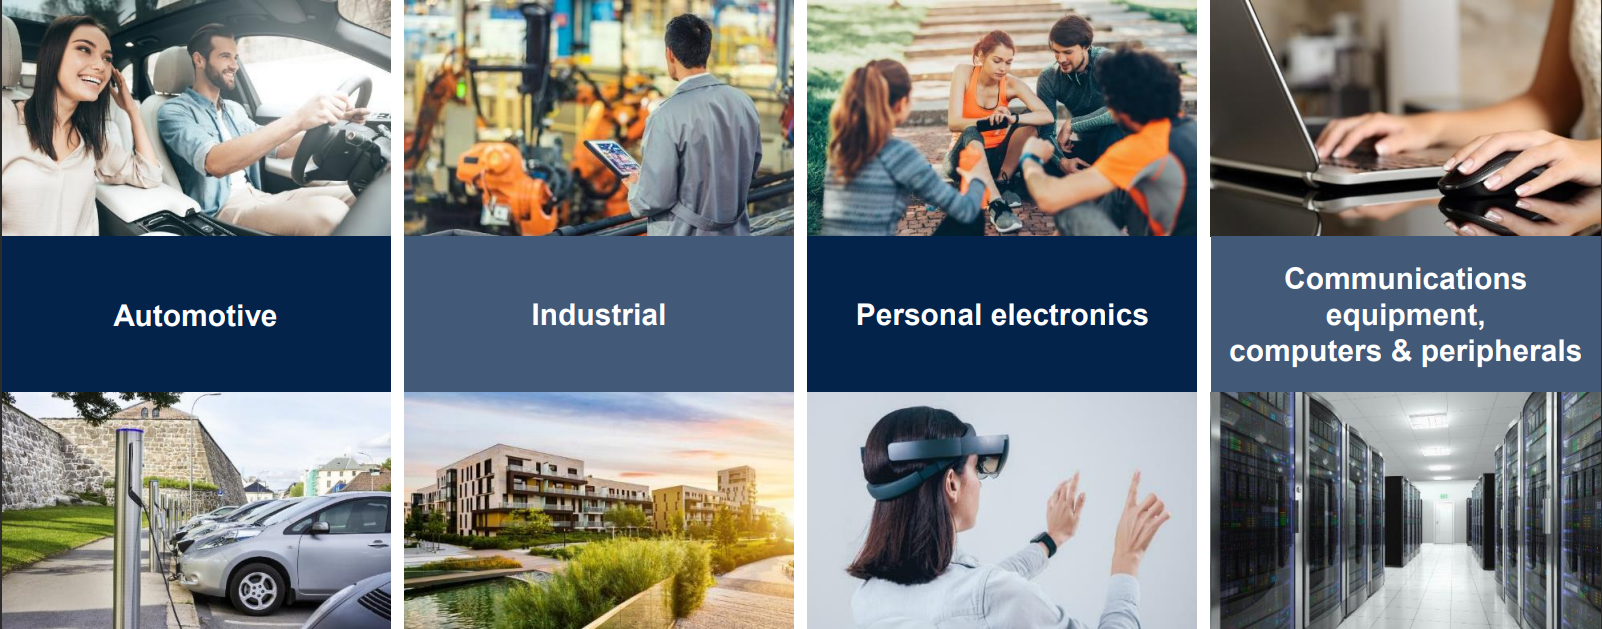
\includegraphics[width=16cm]{end markets.png}
  \caption{STMicroelectronics Activity Sectors}
  \label{fig:st_activities}
\end{figure}

\subsection{Global Presence}

STMicroelectronics operates in more than 35 countries, with a strong presence in key markets around the world. Figure \ref{fig:map} illustrates the company's global network, which includes \cite{st_comp}:

\begin{itemize}
    \item \textbf{Manufacturing Sites:} ST has 14 main manufacturing sites, strategically located to serve its global customer base efficiently.
    \item \textbf{Sales \& Marketing Offices:} With a network of sales and marketing offices, ST provides localized support and services to its customers.
    \item \textbf{R\&D Centers:} ST's R\&D centers are spread across the globe, fostering innovation and collaboration.
\end{itemize}

\begin{figure}[H]
  \centering
  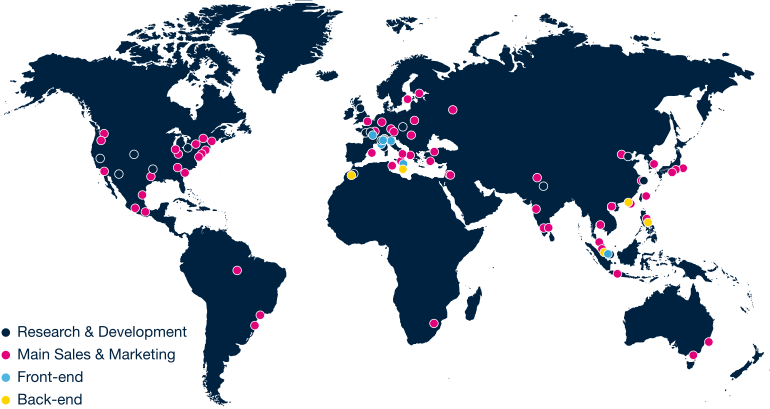
\includegraphics[width=16cm]{st map.png}
  \caption{STMicroelectronics Worldwide Presence}
  \label{fig:map}
\end{figure}

\subsection{ST Tunis}

The STMicroelectronics Tunis site, located in the El Ghazela Technopark, employs over 100 professionals in various fields such as tools, applications, quality, and support functions. The facility is involved in all stages of the microelectronics industry, from initial circuit design to final verification before mass production.

With expertise in both hardware and software, the Tunis center's activities include electronic circuit design, software tool development, application software support, and the electrical validation and verification of new circuits. This diverse skill set allows the center to contribute significantly to ST's global operations. Figure \ref{fig:st_tn} shows the site.

 \begin{figure}[htp]
  \centering
  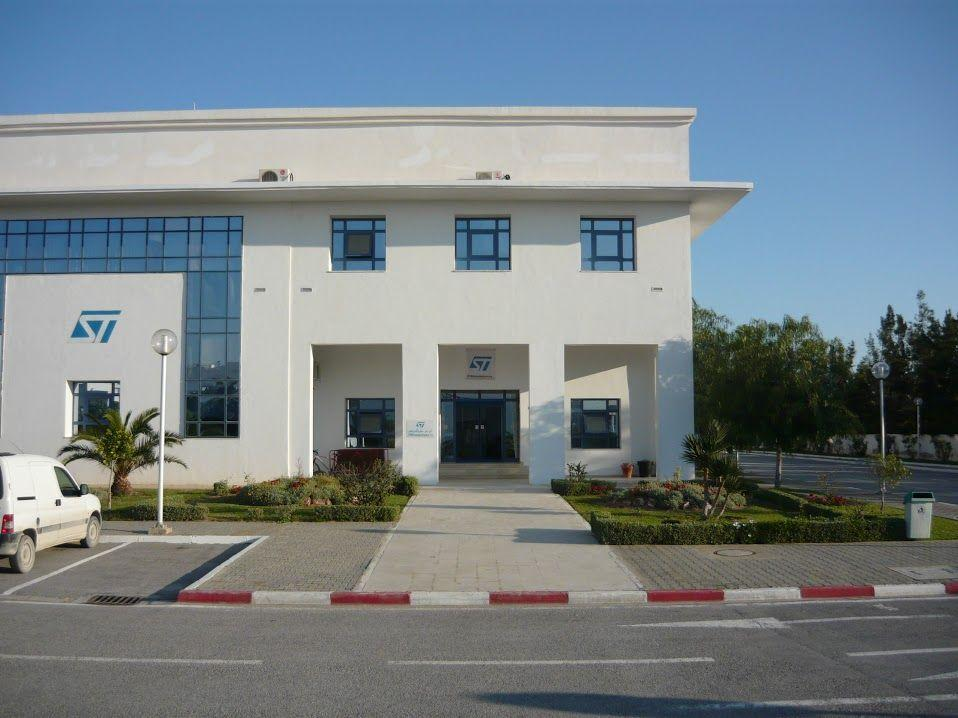
\includegraphics[width=10cm]{stmicroelectronics-tunis-site.jpg}
  \caption{STMicroelectronics Tunis}
  \label{fig:st_tn}
\end{figure}


\subsection{Application \& Product Support Team}
The Application \& Product Support team is dedicated to delivering comprehensive customer support while managing and publishing STM32 product documentation. Their role includes providing in-depth technical support for ST’s tools and products, helping customers troubleshoot problems and optimize their use of these technologies. They ensure the accuracy, clarity, and consistency of all technical documentation, which is regularly updated to reflect the latest developments and innovations.

The team is also involved in enhancing and maintaining existing products, as well as defining new products, derivatives, and application references to meet evolving market needs. Additionally, they lead initiatives related to intellectual property applications, offering specific support through the development of application notes, training programs, and other resources that help customers fully understand and utilize ST’s products. This multifaceted approach ensures both customer satisfaction and continuous improvement in the STM32 ecosystem.
\section{Project Context}

\subsection{Problem Statement}
Debugging software offers a unified experience across many chips, vendors and architectures. It achieves this through a common layer of abstraction that presents heterogeneous targets behind a single conceptual model. The abstraction holds for simple primitives such as memory views and breakpoints. It fails for the advanced features, such as reconstructing execution flow, conditional and cross-triggering of debug events, or recovering execution history after a failure. Those features do not generalize, since each is tightly coupled to a vendor-specific implementation.

The gap between what a chip provides and what a developer can reach is the central concern of this project.
\subsection{State of the Art}
Debugging an embedded system from a host machine like a computer needs multiple components to work together, starting with the debug interface present on the microcontroller chip, the debugger software, and a hardware debug probe that links the microcontroller and the host machine.

\begin{table}[htbp]
    \centering
    \caption{Embedded Systems IDE Vendors}
    \label{tab:ide_vendors}
    \begin{tabularx}{\linewidth}{| @{}>{\hsize=1.05\hsize\bfseries}Y | >{\hsize=1.05\hsize}Y | >{\hsize=0.95\hsize}Y | >{\hsize=0.95\hsize}Y | >{\hsize=1.0\hsize}Y@{} |}
        \hline
        Vendor & \textbf{Toolchain} & \textbf{Debugger} & \textbf{Debug server} & \textbf{Debug probe} \\
        \hline
        IAR & IAR toolchain (ICCARM) & C-SPY & Integrated & I-jet, I-jet Trace \\
        \hline
        Keil & Arm Compiler (armcc, armclang) & \textmu Vision debugger & Integrated & ULINK family \\
        \hline
        SEGGER & SEGGER toolchain & Ozone & J-Link GDB server & J-Link, J-Trace \\
        \hline
        STMicroelectronics & ST-Clang & GDB & ST-LINK GDB server & ST-LINK \\
        \hline
        Free & GCC, LLVM & GDB or LLDB & OpenOCD or pyOCD & CMSIS-DAP \\
        \hline
    \end{tabularx}
\end{table}
The features the proprietary debuggers provide for devices based on the Arm architecture are worth examining in turn. ST's tools are specialized forks of open-source projects and are therefore excluded from this comparison.

\begin{table}[htbp]
    \centering
    \begin{threeparttable}
    \caption{Debugger Features}
    \label{tab:debugger_features}
    \begin{tabularx}{\linewidth}{| @{}>{\hsize=1.3\hsize\bfseries}Y | >{\hsize=0.9\hsize}Y | >{\hsize=0.9\hsize}Y | >{\hsize=0.9\hsize}Y@{} |}
        \hline
        Feature & \textbf{IAR} & \textbf{Keil} & \textbf{SEGGER} \\
        \hline
        ITM trace & \cmark & \cmark & \cmark\tnote{1} \\
        \hline
        Instruction trace & \cmark & \cmark & \cmark \\
        \hline
        CTI support & \xmark & \xmark & \xmark \\
        \hline
        Scripting interface & \cmark & \cmark & \cmark \\
        \hline
        Multi-core debugging & Limited & Limited & Limited \\
        \hline
        IDE coupling & \cmark\tnote{2} & \cmark & \xmark \\
        \hline
    \end{tabularx}
    \begin{tablenotes}
        \item[1] Supports UART encoding only
        \item[2] Implemented in the IDE, and able to work as a standalone server
    \end{tablenotes}
    \end{threeparttable}
\end{table}

\subsection{Critique of Current State of the Art}
\label{subsec:critique}
Vendor IDEs expose a fixed set of tracing settings through their interface. they therefore reapplies the fixed configuration at every resume, which is consistent behavior from the point of view of the tool and leaves a developer no way to hold a configuration of their own.

Debug probes impose limitations of their own. IAR, Keil and SEGGER each supply two versions of their probe, a base model and an extended model that captures trace through dedicated pins.

\begin{table}[htbp]
    \centering
    \begin{threeparttable}
    \caption{Debug Probe Limitations}
    \label{tab:debug_probe_limitations}
        \begin{tabularx}{\linewidth}{| @{}>{\bfseries}Y | Y | Y | Y | Y@{} |}
        \hline
        Probe & \textbf{Supported by IAR} & \textbf{Supported by Keil} & \textbf{Supported by SEGGER} & \textbf{Trace pin capture} \\
        \hline
        I-jet & \cmark & \xmark & \xmark & \cmark \tnote{1} \\
        \hline
        ULINK & \xmark & \cmark & \xmark & \cmark \tnote{1} \\
        \hline
        J-Link, J-Trace & \cmark & \cmark & \cmark & \cmark \tnote{1} \\
        \hline
        ST-LINK & \cmark & \cmark & \cmark & \xmark \\
        \hline
        CMSIS-DAP & \cmark & \cmark & \cmark & \xmark \\
        \hline
    \end{tabularx}
    \begin{tablenotes}
        \item[1] Given the appropriate model
        \item[2] Established by evaluating the probes during this work, in the versions given in Table \ref{tab:debugger_features}.
    \end{tablenotes}
    \end{threeparttable}
\end{table}

Among the tools examined, none exposes on-chip trace capture through a probe other than its own, none decodes trace capture outside of a live debug session, or a capture obtained by other means than a debug probe.

\subsection{Proposed Solution}
The proposed solution takes the form of four results.

An application note assembles into one document the procedure for using instruction trace on these devices.

An implementation of drivers that allow a host machine to configure the concerned trace and debug components.

A pipeline for trace decoding processing and analysis that is decoupled from the trace extraction means, and of a debugging session, allowing for offline trace analysis.

A debug engine carries that chain alongside the conventional debugging capabilities and presents the result inside a development tool during a live session.

\section{Conclusion}
This first chapter introduces the host organization, STMicroelectronics, and provides the context and objectives of the project. It sets the stage for understanding the foundational aspects of the project and its significance.

        \clearpage

        \chapter{Foundations of Debugging and Instruction Trace}
\chaplabel{ch:theory}

\section*{Introduction}
This chapter establishes the concepts on which the remainder of this report depends. The presentation moves from the general to the particular. It opens with the definition of debugging and of the tool that performs it, then describes the operations a debugger provides and the categories into which debugging techniques fall. It continues with the representation of a compiled program, then narrows to microcontrollers, to the ARM M-profile architecture, to the debug and trace infrastructure that ARM defines for it, and finally to the implementation of that infrastructure in STM32 devices.

\section{Debugging Fundamentals}
\label{sec:fundamentals}

\subsection{Bugs, Specifications and Defects}
\label{subsec:bugs}
A defect is a condition in a program that causes its behavior to violate its specification. Debugging is the process of investigating program behavior to identify the cause of such defects. The term \textit{bug} is used interchangeably with defect.

Identifying a defect requires a specification to compare against. A program required to toggle a LED once per second provides a simple example. A LED that remains static, or that toggles at a different rate, is a case of a program violating its specification.

A specification states an end result, and that result implies intermediate behavior. Toggling a LED on a microcontroller requires initializing the device, configuring its power supply and clock tree, and writing to the registers that drive the output pin. A fault at any of these stages produces the same observable symptom, namely a LED that does not blink at the required rate. Writing to an incorrect register and omitting the clock configuration are distinct defects with identical symptoms.

Locating a defect requires identifying the stage at which the program departs from its specification. Debugging therefore depends on a means of observing the state of the system, either by executing the program under a debugger or by instrumenting the program to report it through logging.

\subsection{Anatomy of a Debugger}
\label{subsec:anatomy}
A debugger is a software system that provides controlled interactions with a target system generally referred to as a \textit{debuggee} for the purpose of examining and modifying its state.

Providing these operations requires two broad classes of work. The first is interpreting the representation of the program, which covers the machine code and the debug information held in the executable image. The second is interacting with the target.

A further distinction concerns presentation. The \textit{frontend} is the program that provides the user interface through which debug operations are requested and the state of the debuggee is displayed. The \textit{backend} is the part that carries out the two classes of work mentioned above and maintains the state of a debugging session. For embedded systems such as a microcontroller, a hardware component named \textit{debug probe} or \textit{hardware probe} is generally needed to connect the host machine and the target debuggee. This element represents an intermediary communication channel between both systems. Figure \ref{fig:anatomy} shows the decomposition.

\begin{figure}[H]
    \centering
    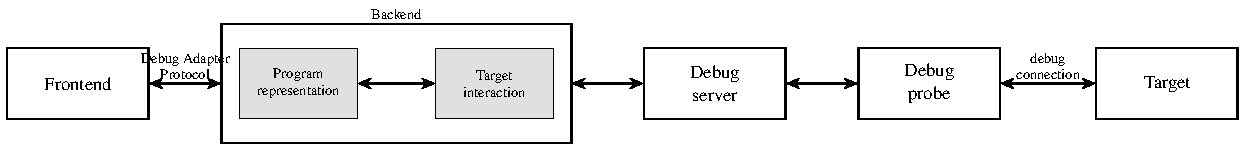
\includegraphics[width=\linewidth]{fig_debugger_anatomy.pdf}
    \caption{Conceptual decomposition of a debugger}
    \label{fig:anatomy}
\end{figure}
Each junction in this chain is governed by a protocol. The connection between the probe and the target depends on the architecture of the device and is the subject of Section \ref{sec:arm_debug}. The decomposition given here is conceptual, and a given system may distribute the responsibilities differently.

\subsection{The Debug Adapter Protocol}
\label{subsec:dap}
The Debug Adapter Protocol defines the messages exchanged between a development tool and a \textit{debug adapter}, a component that translates those messages into operations on the debugging mechanism beneath it \cite{dap_spec}. A debugger is therefore not required to implement the protocol itself, since the adapter stands between the protocol and the interface the debugger already exposes \cite{dap_spec}.

The protocol describes the entities the developer works with, namely source files, line numbers, variables, threads and stack frames. It further permits requests and events outside the standard set, which allows an adapter to expose capabilities that the protocol does not describe.

\subsection{The GDB Remote Serial Protocol}
\label{subsec:rsp}
The GDB RSP is a point-to-point text-based communication protocol defined as part of the GNU debugger \cite{gdb_rsp}, that allows a debugger to connect to a remote target.

The debugger is the client and the target is the server. Every exchange is initiated by the client, and every transaction must be completed before initiating the next one\cite{gdb_rsp}.

The operations the protocol carries include reading and writing the processor registers, reading and writing memory, inserting and removing breakpoints, resuming execution and executing a single instruction \cite{gdb_rsp}.

A debugger may extend the set of packets. LLDB for example, defines packets of its own alongside the standard set \cite{lldb_rsp}.

\section{Debug Primitives}
\label{sec:primitives}
In this work, \textit{debug primitives} refer to the fundamental operations that a debugger exposes. Each is defined here in general terms.

\subsection{Run Control}
Run control provides mechanisms for starting, stopping and controlling the execution of the debuggee. Halting suspends execution and leaves the state of the program unchanged. Resuming returns the program to normal execution from the point at which it was suspended.

Stepping executes a limited portion of the program and then halts again. The size of that portion depends on the granularity requested, mainly, a single instruction or one source statement, which usually amounts to several machine instructions \cite{markusson2008}. Further granularities are common, such as advancing over a complete function call rather than entering it.

\subsection{Breakpoints: Software and Hardware}
A breakpoint is an artificial stopping point inserted into a program for the purpose of debugging. When execution reaches the breakpoint, the program is suspended, after which execution may continue from the point at which it was suspended \cite{markusson2008}.

The mechanisms by which breakpoints are implemented are divided into two categories:

A \textit{software breakpoint} replaces the instruction at the target address with a dedicated instruction that raises a debug event, and restores the original instruction once the breakpoint is removed.

A \textit{hardware breakpoint} instead configures dedicated hardware components on the device such as comparators that watch the address of instructions fetched and raises a debug event on a match without modifying the program. Figure \ref{fig:breakpoints} contrasts the two mechanisms.

\begin{figure}[H]
    \centering
    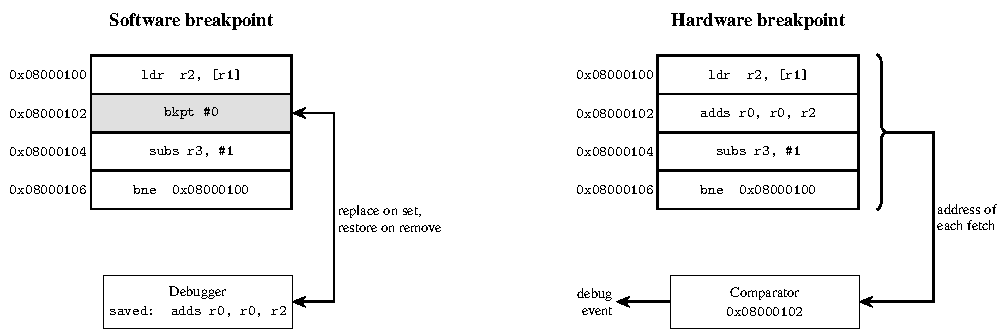
\includegraphics[width=\linewidth]{fig_breakpoints.pdf}
    \caption{Software and hardware breakpoint mechanisms}
    \label{fig:breakpoints}
\end{figure}

\subsection{State Inspection: Registers, Memory and Variables}
The state of a program is observed through two elementary operations, which are reading the processor registers and reading memory \cite{markusson2008}.

These two operations are independent of the program, as neither carries the name, the type or the extent of the variable present in the source code. Presenting a variable therefore requires three further pieces of information, and is generally supplied by the debug information described in Section \ref{subsec:dwarf}.

\subsection{Call Stacks and Unwinding}
 The call stack is the sequence of subroutine activations that are in progress. An activation consists of a code location within the subroutine, an area of memory allocated on the stack termed a call frame, and the set of registers in use by the subroutine at that location \cite{dwarf5}.

Only the innermost activation is directly visible, since the processor registers describe that activation alone. Reaching the others requires \textit{unwinding}, which proceeds one frame at a time. Starting from the current activation, the debugger restores the registers that this activation preserved and computes the address of the preceding call frame together with the corresponding code location\cite{dwarf5}.

\subsection{Disassembly}
Disassembly is the translation of the bytes held in the executable memory of the target back into machine instructions.

Disassembly serves two purposes in a debugger. It allows a developer to inspect code for which no source is available, and it allows the machine instructions produced by the compiler to be compared against the source statement they were generated from.

\section{Classes of Debugging}
\label{sec:classes}
Debugging techniques are grouped along several independent axes, and a given technique may occupy a position on each of them.

\subsection{Intrusive and Non-Intrusive Debugging}
\label{subsec:intrusive}
A debug technique is termed intrusive, or invasive, when applying it alters the behavior of the program under examination. It is termed non-intrusive when it does not. Halting the processor and executing debug code through dedicated exceptions are presented as invasive mechanisms, whereas program trace and profiling are presented as non-invasive\cite{armv7m_arm}.

A program that meets a timing requirement when running freely may fail that requirement when it is halted at a breakpoint, and a defect that depends on the relative timing of an interrupt and the main program may cease to appear once the timing is disturbed. Adding logging statements has a comparable effect.

\subsection{Live and Post-Mortem Debugging}
Live debugging examines a program while it is running or halted under the control of a debugger. The developer forms a hypothesis, sets a breakpoint, inspects state and repeats. The technique requires the defect to be reproducible while the debugger is attached.

Post-mortem debugging examines a record produced during execution and analyzed once that execution has finished. The term carries no implication that the program failed, since the record may equally describe a run that completed normally. The record may be a set of fault status registers, a region of memory preserved across a fault, a log, or a buffer of captured trace. No interaction with the program is possible during the analysis, so the analysis is limited to what the record contains. The technique applies where live debugging does not, for instance where a failure appears rarely, or where attaching a debugger would itself prevent it from occurring.

\subsection{Run-Control and Trace-Based Debugging}
\label{subsec:runstop}
A debugger that supports the operations of Section \ref{sec:primitives} is termed a run-stop debugger, or a run-time control debugger\cite{markusson2008}. The developer directs the investigation by deciding where to stop and what to examine.

Tracing follows the opposite order. Tracing records the program flow and the data accesses of the program while it runs, and the recorded information is used at a later stage to perform run-stop debugging \cite{markusson2008}.

The two approaches answer different questions. A run-stop debugger answers what the state is at a chosen point. Tracing answers what the program did over an interval, including the path taken to reach a point of failure.

\section{Program Representation}
\label{sec:program_repr}
This section describes how a compiled program is stored, what the mapping between source-code and machine-code contains, and how machine code is translated back into instructions.

\subsection{The Embedded Build Model}
A program written in a high-level language passes through several tools before it can execute. The compiler translates each source file into an object file containing machine code together with unresolved references to entities defined elsewhere. The linker combines the object files, resolves those references, assigns an address to every function and variable, producing an executable image.

Embedded development has different properties in this aspect to host machines, mainly the fact that addresses are fixed at link time and describe a physical device.

The debugger consumes the same image. extracting machine code to be disassembled, the addresses at which functions and variables reside, and the debug information relating those addresses to the source.

\subsection{The ELF Format}
The Executable and Linkable Format (ELF) is the object file format used by the toolchains considered in this work. ARM defines a processor-specific supplement to it for its own architecture \cite{aaelf32}.

\subsubsection{Segments, Sections and the Loadable Image}
An ELF file describes its contents in two manners. The section header table describes the file as a set of \textit{sections}, which groups related content under a name and a type, so that machine code, initialized data, uninitialized data and debug information each occupy sections of their own. The program header table describes the file as a set of \textit{segments}, which is the view used when the program is loaded. A segment of loadable type identifies a range of the file together with the address at which that range must appear in memory.

\subsubsection{Symbol Tables}
A symbol table is a data structure where each symbol in the source code is associated with the necessary information for its functioning. Each entry records the name of an entity, its address, the number of bytes it occupies, and its kind, which distinguishes a function from a data object among other categories.

\subsubsection{ARM Mapping and Tagging Symbols}
\label{subsec:mapping_symbols}
A section of an ARM ELF file can contain a mixture of ARM code, Thumb code and data. The mapping and tagging symbols are used in the symbols table to denote the start of a specific section of the appropriate type.

\begin{table}[H]
    \centering
    \caption{ARM Mapping Symbols}
    \label{tab:arm_map_tag}
    \begin{tabularx}{\linewidth}{| @{}>{\hsize=0.3\hsize\bfseries}Y | >{\hsize=1.7\hsize}Y@{} |}
        \hline
        Symbol & \textbf{Definition} \\
        \hline
        \$a & Denotes the start of a region of code containing ARM instructions. \\
        \hline
        \$t & Denotes the start of a region of code containing Thumb instructions. \\
        \hline
        \$d & Denotes the start of a region of data.\\
        \hline
    \end{tabularx}
\end{table}

\subsection{DWARF Debug Information}
\label{subsec:dwarf}
DWARF is the debug format used by the toolchains considered here. It describes a program as a tree in which nodes represent functions, data and types, provides a mapping between executable instructions and the corresponding source code lines, and describes how to unwind the stack \cite{markusson2008}. It is stored in dedicated sections of the ELF file. Table \ref{tab:dwarf} states the constructs it defines and the debugger operation each supports.

\begin{table}[H]
    \centering
    \caption{DWARF constructs and the operations they support}
    \label{tab:dwarf}
    \begin{tabularx}{\linewidth}{| @{}>{\hsize=0.7\hsize\bfseries}Y | >{\hsize=1.2\hsize}Y | >{\hsize=1.1\hsize}Y@{} |}
        \hline
        Construct & \textbf{What it describes} & \textbf{Operation it supports} \\
        \hline
        Debugging information entries & The program as a tree of functions, data and types, nested as the source is nested. & Determining which names are visible at a given point. \\
        \hline
        Line number program & The correspondence between instruction addresses and source lines. & Presenting a location in source terms and stepping from line to line. \\
        \hline
        Inlined subroutines & The expansion of a subroutine at its call site, and the chain of source locations that results. & Reporting the call site rather than the expanded code alone. \\
        \hline
        Type descriptions & How the bytes belonging to a variable are to be interpreted. & Displaying a variable rather than a sequence of bytes. \\
        \hline
        Location descriptions & Where an object resides, which may change over its lifetime. & Finding a variable at the current point of execution. \\
        \hline
        Call frame information & Where registers are saved and how the address of the preceding frame is computed. & Unwinding the call stack. \\
        \hline
    \end{tabularx}
\end{table}

\section{Microcontrollers}
\label{sec:microcontrollers}
A microcontroller is a system that integrates a processor, its memories and a set of peripherals within a single component. It cannot host a debugger, since it has neither the memory to hold one nor the means for a developer to operate one on it \cite{markusson2008}.

\subsection{Device Description: CMSIS-SVD}
The CMSIS System View Description format formalizes the description of the system contained in ARM Cortex processor-based devices, in particular, the memory mapped registers of peripherals. The detail contained in system view descriptions is comparable to the data in device reference manuals. The information ranges from high level functional descriptions of a peripheral all the way down to the definition and purpose of an individual bit field in a memory mapped register. \cite{cmsis_svd}.

The format is based on XML and describes a single device per file. A device consists of a processor and at least one peripheral, each peripheral contains at least one register, and a register may consist of one or more fields \cite{cmsis_svd}. Each level carries attributes, such as the address of a register, its reset value, the width and position of each field, whether a field may be read or written, and the meaning of particular field values.\cite{cmsis_svd}.

\section{The ARM Cortex-M Architecture}
\label{sec:cortexm}
This section describes the parts of the architecture that the debug and trace infrastructure of Sections \ref{sec:arm_debug} and \ref{sec:coresight} depends upon.

\subsection{ARM Architecture}
ARM divides its architecture into three profiles, addressed to different classes of application. The A-profile targets systems running general-purpose operating systems, the R-profile targets systems with real-time requirements, and the M-profile targets microcontrollers.

\subsection{Register Model and the Thumb Instruction Set}
The M-profile presents thirteen general-purpose registers, a stack pointer, a link register, a program counter, and a program status register carrying the condition flags and the current execution state.

The M-profile executes the Thumb instruction set only.

\subsection{Exception Model and Vector Table}
In ARM architectures, an exception is defined as any events that suspends the currently executing program, this can originate from a peripheral signal termed an interrupt, a fault, or a software request.

An exception requires a handler, which is a subroutine that is executed whenever the exception occurs. The addresses of the handlers are stored contiguously in a table termed the Vector Table, which is indexed by the exception number to retrieve the appropriate handler.

\subsection{System Address Map}
The M-profile defines a default address map that assigns a purpose to each region of the address space. Distinct regions are reserved for code, for on-chip static memory, for peripherals, and for external memory and devices \cite{armv7m_arm, armv8m_arm}.

A further region is reserved for the Private Peripheral Bus (PPB), which holds the registers of the system and debug components belonging to the processor \cite{armv7m_arm, armv8m_arm}.

\begin{figure}[H]
    \centering
    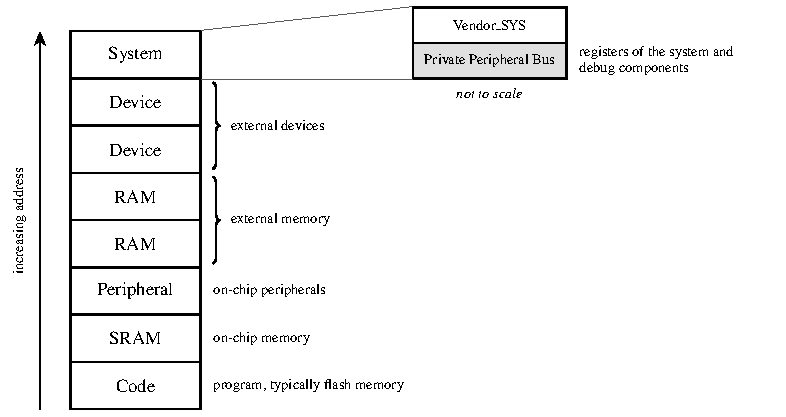
\includegraphics[width=0.88\linewidth]{fig_address_map.pdf}
    \caption[The M-profile system address map]{The M-profile system address map \cite{armv7m_arm}}
    \label{fig:addrmap}
\end{figure}
\subsection{AMBA Buses and their Roles in Debug}
\label{subsec:amba}
The components of an ARM device are connected by buses defined in the Advanced Microcontroller Bus Architecture (AMBA). Table \ref{tab:amba} states the four most common ones.

\begin{table}[H]
    \centering
    \caption{AMBA buses and their roles in debug and trace}
    \label{tab:amba}
    \begin{tabularx}{\linewidth}{| @{}>{\hsize=0.35\hsize\bfseries}Y | >{\hsize=0.9\hsize}Y | >{\hsize=1.75\hsize}Y@{} |}
        \hline
        Bus & \textbf{Name} & \textbf{Role} \\
        \hline
        APB & Advanced Peripheral Bus & Carries configuration accesses to debug components. Transactions arriving from a debug connection are converted into APB transactions and transported to each of the components the debugger must access \cite{coresight_guide}. \\
        \hline
        AHB & Advanced High-performance Bus & The protocol through which the debug registers of a Cortex-M processor are commonly reached. Accesses may be directed to all locations in the memory space of the processor rather than to the debug registers alone \cite{coresight_guide}. \\
        \hline
        AXI & Advanced eXtensible Interface & Carries accesses into the main functional memory space of the devices that implement it, bypassing the caches and the memory map controls of the processor \cite{coresight_guide}. Where a device routes captured trace into system memory, this is also the interface over which that trace is written, as Section \ref{subsec:onchip_sinks} describes. \\
        \hline
        ATB & Advanced Trace Bus & Reserved for trace. It is a common bus used by the trace components to pass trace data in a data-agnostic format \cite{atb_spec}, which is what allows one infrastructure to transport several kinds of trace. \\
        \hline
    \end{tabularx}
\end{table}

\section{The ARM Debug Architecture}
\label{sec:arm_debug}
Section \ref{subsec:anatomy} left the junction between the probe and the target undescribed. This section describes the specification that governs it and the debug logic it reaches.

\subsection{The ARM Debug Interface}
The ARM Debug Interface (ADI) defines the means by which a debugger accesses the debug functionality provided by debug components in an embedded system on chip \cite{adiv5}.

An implementation of that specification within a device is termed a Debug Access Port (DAP), which provides a debugger with a standard interface for accessing debug resources in systems that expose their debug information by resource-specific methods \cite{adiv5}.

The Debug Access Port presents one interface to the debugger and performs the resource-specific access on its behalf. It is composed of two kinds of elements, a Debug Port and one or more Access Ports, Figure \ref{fig:dap} shows an example configuration of a DAP.

\begin{figure}[H]
    \centering
    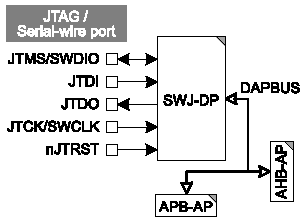
\includegraphics[width=0.62\linewidth]{dap_structure.pdf}
    \caption[Structure of a Debug Access Port]{Structure of a Debug Access Port\cite{rm0477}}
    \label{fig:dap}
\end{figure}

\subsection{Debug Port: JTAG and SWD}
A Debug Port provides four things\cite{adiv5}:
\begin{itemize}
    \item The external physical connection to the interface.
    \item A method of obtaining the identification code of the Debug Access Port.
    \item The methods by which the debugger accesses the Debug Port and Access Port registers.
    \item A method of aborting a register access that appears to have failed.
\end{itemize}

There are three types of Debug Ports,
\begin{itemize}
    \item JTAG Debug Port is accessed by scan chains compliant with IEEE 1149.1.
    \item Serial Wire Debug Port (SWD) is a two-pin serial interface using a packet-based protocol to read and write registers.
    \item SWJ Debug Port which combines the two above\cite{adiv5}.
\end{itemize}

The debugger drives serial accesses that scan values into registers inside the Debug Port, which are then converted into bus transactions directed at an Access Port register \cite{coresight_guide}.

\subsection{Access Ports and the Memory Access Port}
An Access Port uses a resource-specific transport mechanism to access debug information in the system, and passes that information to the Debug Port \cite{adiv5}. A Debug Access Port contains at least one Access Port and may contain several \cite{adiv5}, each driving a different memory space, with the type of Access Port determined by the bus protocol required for that space \cite{coresight_guide}.

\subsection{Component Identification and ROM Tables}
CoreSight designates two mechanisms that allow a debugger to discover the debugging capabilities of an unfamiliar device.

The first is a common register layout. A component compliant with the CoreSight architecture occupies a block with a size that is a multiple of four kilobytes, divided between a set of predefined management registers and a set of registers specific to the device \cite{coresight_guide}.

The second is ROM tables. A ROM table always occupies four kilobytes and is part of the address space of the memory system connected to an AP \cite{adiv5}. Its entries point to the components present, and one bit of each entry indicates whether the corresponding component is implemented \cite{armv7m_arm, armv8m_arm}.

\subsection{Halting Debug Control}
On an M-profile device, halting debug capabilities are controlled by the three memory-mapped registers described in table \ref{tab:halting}\cite{armv7m_arm, armv8m_arm}.

\begin{table}[H]
    \centering
    \caption{Registers governing halting debug}
    \label{tab:halting}
    \begin{tabularx}{\linewidth}{| @{}>{\hsize=0.5\hsize\bfseries}Y | >{\hsize=0.75\hsize}Y | >{\hsize=1.75\hsize}Y@{} |}
        \hline
        Register & \textbf{Control} & \textbf{Effect} \\
        \hline
        \multirow{5}{*}{DHCSR} & C\_DEBUGEN & Enables halting debug, after which a debug event halts the processor in Debug state. \\
        \cline{2-3}
        & C\_HALT & Requests a halt when written as one, and a resume when written as zero. The processor also sets it on entry to Debug state. \\
        \cline{2-3}
        & C\_STEP & Requests a single step. \\
        \cline{2-3}
        & C\_MASKINTS & Prevents configurable interrupts from being taken during a step, which is what allows a step to remain within the statement under examination. \\
        \cline{2-3}
        & S\_HALT & Reports that the processor is in Debug state. Read-only. \\
        \hline
        \multirow{3}{*}{DEMCR} & MON\_EN & Enables the DebugMonitor exception, the alternative to halting. \\
        \cline{2-3}
        & Vector catch & ARMs the mechanism described in Section \ref{subsec:reset}. \\
        \cline{2-3}
        & TRCENA & Governs the trace components. \\
        \hline
        DFSR & One bit per event & Reports why execution stopped, distinguishing an internal halt request, a breakpoint, a watchpoint match, a vector catch and an external debug request. A debugger reads it after a halt in order to report the cause to the developer. Each bit is cleared by writing one. \\
        \hline
    \end{tabularx}
\end{table}

\subsection{Reset Types and Vector Catch}
\label{subsec:reset}
M-profile architectures define two types of reset, A Local reset is one initiated through the Debug Access Port, and resets only the core and the debug logic, a System reset on the other hand resets the entire SoC.
Vector Catch is a debug mechanism implemented in Cortex-M devices that allows the device to enter Debug State upon exception entry without requiring a breakpoint.
\subsection{Breakpoint and Watchpoint Units}
\label{subsec:fpb_dwt}

The Flash Patch and Breakpoint unit (FPB) is the debug component that implements hardware breakpoints. Its relevant capability is that it can set breakpoints on code held in read-only memory \cite{armv7m_arm}.

The Data Watchpoint and Trace unit (DWT) implements generic comparators that can be configured to provide various functionalities such as watchpoints, data tracing or signaling for external resources. Moreover, these comparators can be configured to signal a match on either an instruction address, a data address or a data value given that the prior comparator is a data address one.

\section{The CoreSight Trace Architecture}
\label{sec:coresight}
This section describes the architecture that ARM defines for trace. CoreSight is the mechanism ARM uses to provide the connectivity between a debugger and a processor, and it defines a set of capabilities that may be designed into a processor or into system-level components \cite{coresight_guide}.

\subsection{Trace Sources, Links and Sinks}
\label{subsec:sls}
Trace components fall into three categories. A trace source is a component that generates trace data. A trace sink is a component that stores or outputs trace data. A trace link is a component that connects trace components together \cite{understanding_trace}. Any trace path in a device is therefore a chain that begins at a source, passes through zero or more links, and terminates at a sink.

Since a design is free to implement any subset of these components, the topology differs from device to device. A debugger consequently needs to know the topology of the particular target before it can configure a trace path \cite{understanding_trace}.

\subsection{Instruction, Data and Instrumentation Trace}
Trace refers to the process of capturing data that illustrates how the components in a design are operating, executing and performing, and the ARM approach usually involves a separate generation component for each type of trace \cite{understanding_trace}. Table \ref{tab:trace_types} states the types that concern this work.

\begin{table}[H]
    \centering
    \caption{Types of trace}
    \label{tab:trace_types}
    \begin{tabularx}{\linewidth}{| @{}>{\hsize=0.7\hsize\bfseries}Y | >{\hsize=1.7\hsize}Y | >{\hsize=0.6\hsize}Y@{} |}
        \hline
        Type & \textbf{What it records} & \textbf{Intrusive} \\
        \hline
        Instruction & The execution history of the processor, and the places where execution behaves unexpectedly \cite{understanding_trace}. This is the type on which this project is based. & \xmark \\
        \hline
        Data & Each data access, together with the address and the value transferred \cite{understanding_trace}. The trace architecture leaves it optional \cite{understanding_trace}. & \xmark \\
        \hline
        Instrumentation & Events and values supplied by the software itself, in the style of a print statement \cite{understanding_trace}. & \cmark \\
        \hline
    \end{tabularx}
\end{table}

Instrumentation trace differs from the other two in that the program must be modified to produce it, which places it on the intrusive side of the distinction of Section \ref{subsec:intrusive}, albeit at a low level of intrusion \cite{armv7m_arm}.

\subsection{Trace Source: the Embedded Trace Macrocell}
\label{subsec:etm}
The component that generates instruction trace is termed a trace unit. It traces the instructions a processor executes and the data those instructions act upon \cite{etmv4_spec}. The implementation ARM supplies for this purpose is the Embedded Trace Macrocell (ETM), which exists in four architecture versions \cite{etmv3_spec,etmv4_spec}. This work treats ETMv4.

\subsubsection{Functions of a Trace Unit}
A trace unit has two main functions. The first is to generate trace, by producing trace streams. The second is to filter those streams, so that tracing may be made active only for particular threads of execution or particular functions \cite{etmv4_spec}.

The second function follows from a property of the first. A processor executes on the order of hundreds of millions of instructions per second, whereas the path that carries the trace has a fixed bandwidth and the storage at its end a fixed size. Filtering lowers the rate at which trace is produced, so that the path and the storage can keep up.

\subsubsection{Trace Streams and Trace Identifiers}
A trace unit conforming to ETMv4 generates an instruction trace element stream and, where data tracing is implemented and enabled, a data trace element stream \cite{etmv4_spec}. The two are independent, and the architecture requires neither that they be captured by the same device nor that their capture be ordered \cite{etmv4_spec}. Interpreting the data stream, however, typically requires the instruction stream to be interpreted as well \cite{etmv4_spec}.

Several streams may share one bus. Each stream therefore carries its own identifier, and Section \ref{subsec:formatter} describes how it travels with the data.

\subsubsection{Trace Elements}
\label{subsec:elements}
A trace unit reports execution as a stream of elements \cite{etmv4_spec}.

The stream does not contain an element for every executed instruction. An element is generated when the processor executes a direct branch, an indirect branch or an instruction synchronization barrier, when it takes or returns from an exception, and when it enters Debug state \cite{etmv4_spec}. A wait-for-interrupt or wait-for-event instruction generates one only where the unit reports that it does \cite{etmv4_spec}. Each element therefore implies the execution of every instruction from the target of the previous element up to the instruction it reports \cite{etmv4_spec}. A conditional branch needs one bit, namely whether it was taken, and the instructions between two branches need none, since the program image already holds them. An \textit{atom} element carries that bit.

Addresses follow the same principle. A branch whose target is encoded in the instruction needs no address in the trace, since the target may be read from the program image. The trace unit therefore omits an address wherever it can be inferred from the program image and from what the stream has already reported, and transmits only those that cannot \cite{etmv4_spec}.

Table \ref{tab:elements} states what each kind of element reports.

\begin{table}[H]
    \centering
    \caption{Kinds of trace element}
    \label{tab:elements}
    \begin{tabularx}{\linewidth}{| @{}>{\hsize=0.75\hsize\bfseries}Y | >{\hsize=1.25\hsize}Y@{} |}
        \hline
        Element & \textbf{What it reports} \\
        \hline
        Atom & Whether a conditional branch was taken. \\
        \hline
        Address & A branch target that cannot be inferred from the program image. \\
        \hline
        Exception and exception return & Entry to an exception and return from it, which occur at an instruction boundary with no branch appearing in the code. \\
        \hline
        Synchronization & Where a packet starts, the configuration of the trace run, and the address from which to begin reading. \\
        \hline
        Overflow & A gap in the trace, and the reason for it. \\
        \hline
        Timestamp and cycle count & Values from a global counter and counts of processor clock cycles. \\
        \hline
    \end{tabularx}
\end{table}

Synchronization elements are generated periodically, which matters because trace held in a circular buffer is overwritten from an arbitrary point. A captured trace is therefore not necessarily continuous, and an analysis must represent a gap explicitly rather than joining the two sides of it \cite{etmv4_spec}. Figure \ref{fig:loop_elements} works the principle through for a loop of four iterations, in which three taken atoms and one not-taken atom stand for sixteen executed instructions.

\begin{figure}[H]
    \centering
    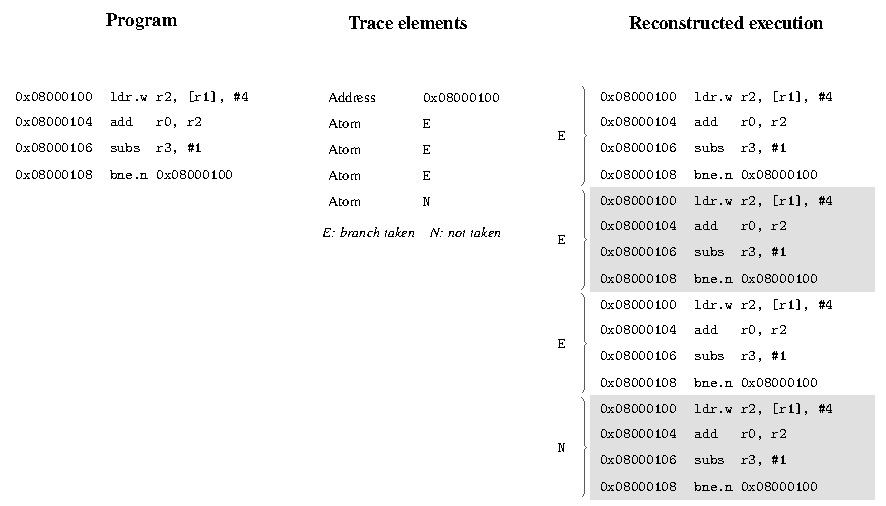
\includegraphics[width=\linewidth]{fig_trace_elements_loop.pdf}
    \caption[Trace elements generated for a short loop]{Trace elements generated for a short loop. Synchronization elements are omitted.}
    \label{fig:loop_elements}
\end{figure}
\subsubsection{Packet Encoding}
\label{subsec:protocols}
Elements are encoded into packets for transmission. A packet is a header byte followed by zero or more payload bytes, and the packet type determines how many \cite{etmv4_spec}. A header is unique within a stream, though the same byte may mean one thing in the instruction stream and another in the data stream, so a decoder must know which stream it reads \cite{etmv4_spec}.

Elements and packets do not correspond one to one. One atom packet may carry several atom elements, and six atom packet formats exist for that purpose \cite{etmv4_spec}. Decoding is therefore two operations, namely recovering packets from the byte stream and expanding them into elements.

The trace alone does not state which instructions executed, since it reports branches and omits the addresses it expects to be inferred. Reconstruction requires the program image \cite{etmv4_spec}. The image must be the exact one the processor ran, as any difference between it and the executed code corrupts the decoded output \cite{understanding_trace}.

\subsection{The CoreSight Trace Formatter}
\label{subsec:formatter}
Where several trace streams share one path, the identity of each must travel with its data. Formatters are the method by which trace source identifiers are wrapped into the output trace data stream, and the format specifies how trace sinks embed the source identifiers carried on the ATB into a single stream \cite{coresight_arch}.

The protocol outputs data in frames of sixteen bytes, arranged as Figure \ref{fig:formatter_frame} shows. The architecture specification gives the meaning of every byte in full \cite{coresight_arch}.

\begin{figure}[H]
    \centering
    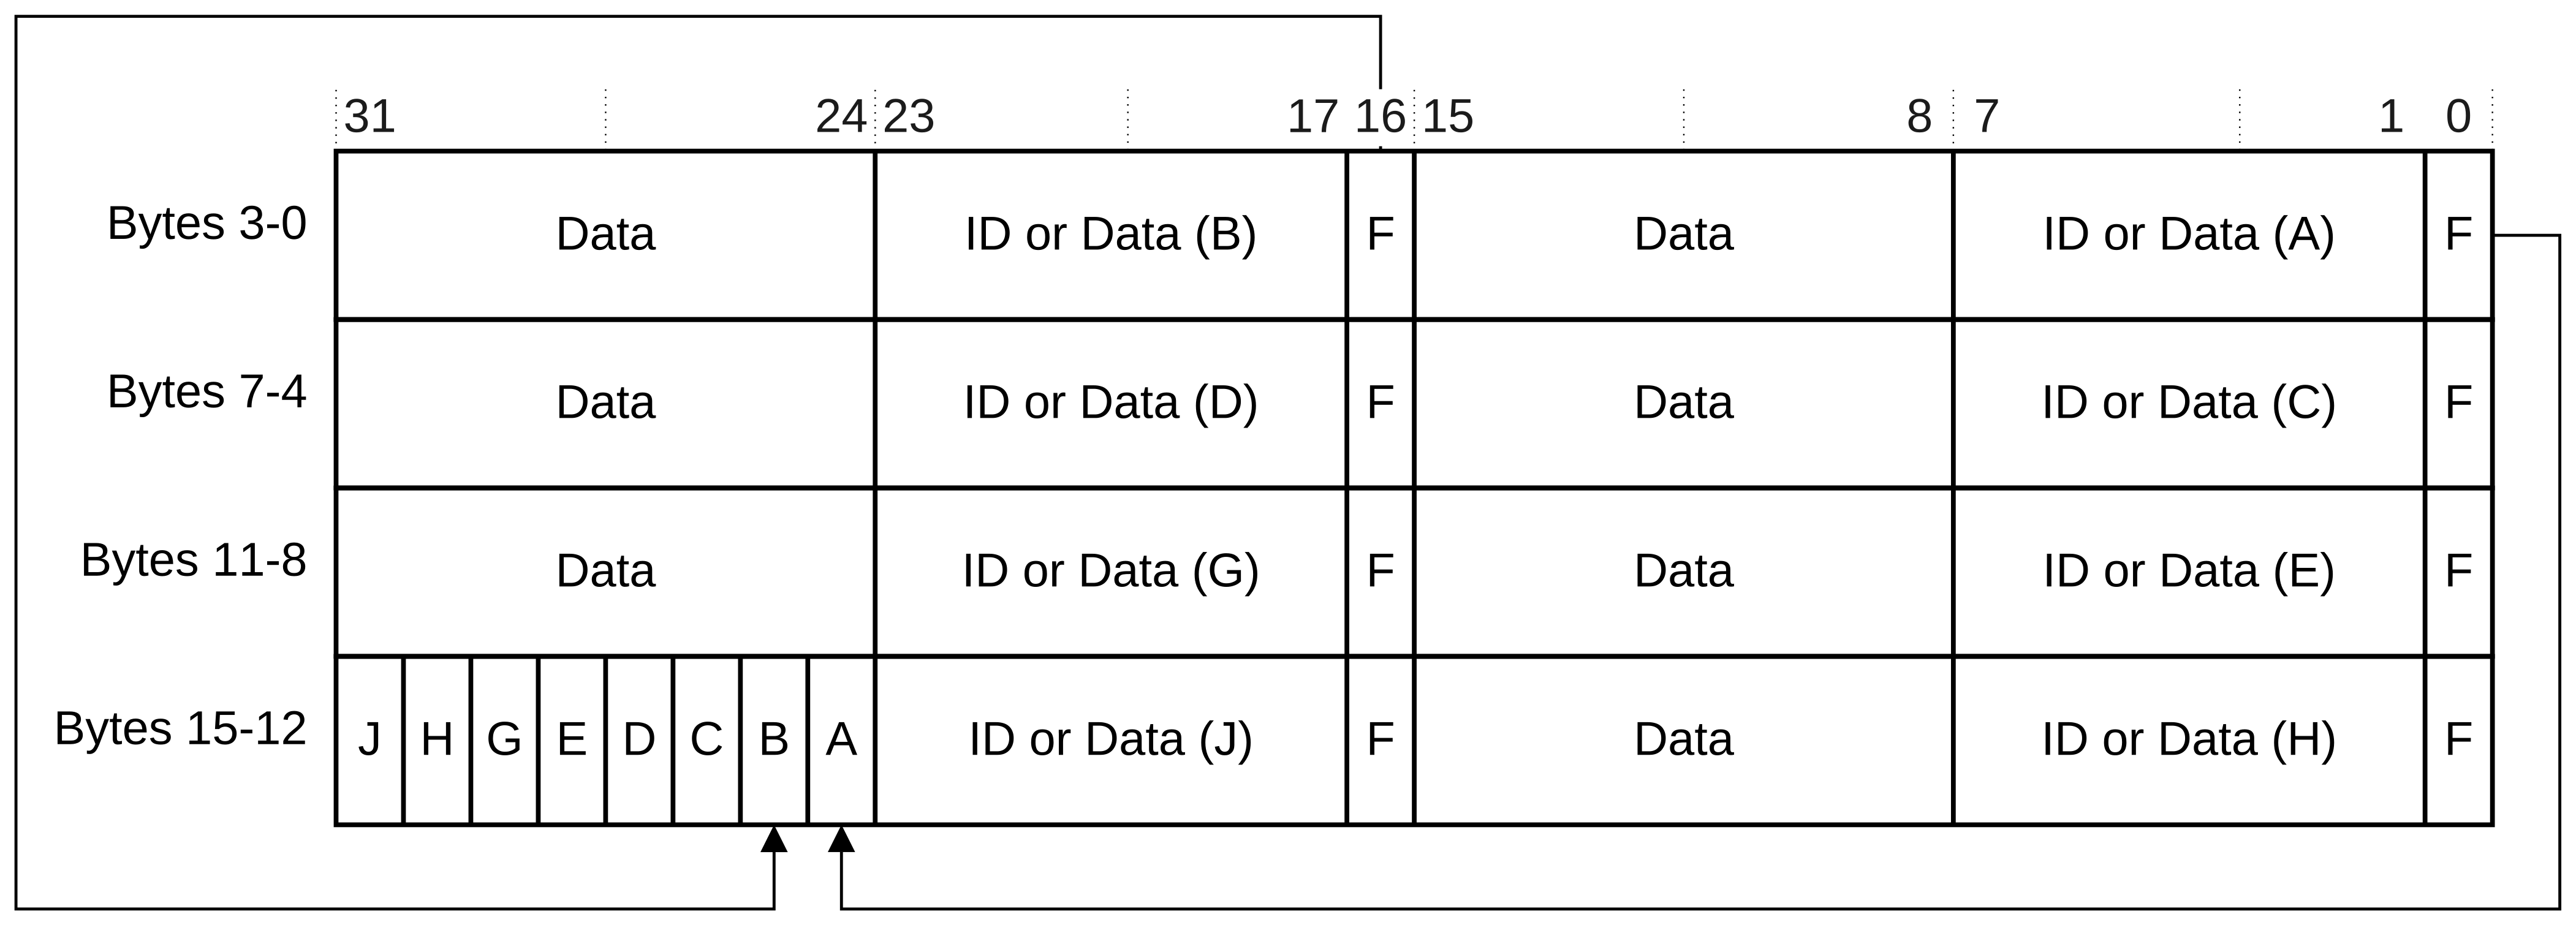
\includegraphics[width=\linewidth]{formatter_frame.png}
    \caption[Structure of a formatter frame]{Structure of a formatter frame \cite{coresight_arch}}
    \label{fig:formatter_frame}
\end{figure}

The design serves several ends at once \cite{coresight_arch}:
\begin{itemize}
    \item Trace from several sources may be merged into a single stream and later separated.
    \item No requirement is placed on the data emitted by the sources.
    \item The result may be stored as a bitstream without separate alignment information.
    \item The result may be decoded even where the start of the trace has been lost.
\end{itemize}

Where only a single trace source is used and the embedded trigger and flow control information is not required, formatting may be disabled to obtain better throughput \cite{coresight_arch}. A decoder must therefore be told whether the stream it receives is formatted, since a formatted stream requires the frames to be unwrapped before the packet decoding of Section \ref{subsec:protocols} may begin.

\subsection{Off-Chip Trace Sinks: TPIU and SWO}
Two families of sink exist, distinguished by where the trace data comes to rest. The first exports it from the device.

The standard component for this purpose is the Trace Port Interface Unit (TPIU), which drives the external pins of a trace port so that capture hardware may receive the data \cite{soc400_trm}. It also inserts source identifiers into the stream and coordinates the stopping of capture when a trigger is received \cite{soc400_trm}.

The limitation of this route is bandwidth. A trace port is a small number of pins running at a fraction of the internal frequency, so it carries far less than the on-chip trace bus and suits a low rate of trace over a long period \cite{coresight_guide}. The Serial Wire Output (SWO) passes trace over a single pin directly to a debugger, at a lower rate still \cite{understanding_trace}.

Two practical constraints follow. Pins must be available on the package and routed on the board, and the capture equipment must be able to receive them, which usually means a probe more capable than the one used for ordinary debugging. Neither constraint is met by every board.

\subsection{On-Chip Trace Sinks: the Trace Memory Controller}
\label{subsec:onchip_sinks}
The second stores it inside the device, which is what the Trace Memory Controller (TMC) does \cite{understanding_trace}.

Two axes describe the component. The configuration is fixed when the design is integrated into a system, and Table \ref{tab:tmc} states the three that exist. The operating mode is chosen when the component is programmed, and Table \ref{tab:tmc_modes} states the three that exist \cite{tmc_trm}.

\begin{table}[H]
    \centering
    \caption{Trace Memory Controller configurations}
    \label{tab:tmc}
    \begin{tabularx}{\linewidth}{| @{}>{\hsize=0.9\hsize\bfseries}Y | >{\hsize=0.85\hsize}Y | >{\hsize=1.3\hsize}Y | >{\hsize=0.95\hsize}Y@{} |}
        \hline
        Configuration & \textbf{Storage} & \textbf{Retrieval} & \textbf{Memory size range} \\
        \hline
        ETB & Dedicated SRAM & Debug bus & 512 bytes to four gigabytes \\
        \hline
        ETF & Dedicated SRAM & Debug bus, or drained over the trace bus & 512 bytes to four gigabytes \\
        \hline
        ETR & System memory, over AXI & Debug bus & The size of the memory region \\
        \hline
    \end{tabularx}
\end{table}

\begin{table}[H]
    \centering
    \caption{Trace Memory Controller operating modes}
    \label{tab:tmc_modes}
    \begin{tabularx}{\linewidth}{| @{}>{\hsize=0.75\hsize\bfseries}Y | >{\hsize=1.65\hsize}Y | >{\hsize=0.6\hsize}Y@{} |}
        \hline
        Mode & \textbf{Description} & \textbf{Configurations} \\
        \hline
        Circular buffer & The storage is used as a circular buffer. Old trace is overwritten once it is full, and nothing may be read until capture has stopped. & ETB, ETF, ETR \\
        \hline
        Hardware FIFO & The component acts as a link between a source and a sink, applying back pressure rather than losing trace. & ETF \\
        \hline
        Software FIFO & The component acts as a queue that a debugger reads over the debug bus while capture continues. & ETB, ETF, ETR \\
        \hline
    \end{tabularx}
\end{table}

The dedicated memory of the ETB and ETF configurations is normally small, so triggering and filtering are usually necessary to ensure that important trace is not lost through wrapping \cite{understanding_trace}.

Table \ref{tab:sink_tradeoff} sets the two routes against each other.

\begin{table}[H]
    \centering
    \caption{On-chip and off-chip trace capture}
    \label{tab:sink_tradeoff}
    \begin{tabularx}{\linewidth}{| @{}>{\hsize=0.7\hsize\bfseries}Y | >{\hsize=1.1\hsize}Y | >{\hsize=1.2\hsize}Y@{} |}
        \hline
        & \textbf{On-chip} & \textbf{Off-chip} \\
        \hline
        Bandwidth & The full internal bus rate & A fraction of the internal rate \\
        \hline
        Size & The size of the memory & The size of the capture device \\
        \hline
        Throughput & Read out after capture & Continuous during capture \\
        \hline
        Extra hardware & None & Trace pins, board routing and a capture probe \\
        \hline
    \end{tabularx}
\end{table}


\section{Debug and Trace Infrastructure in STM32 Microcontrollers}
\label{sec:stm32}
The preceding two sections described what ARM specifies. A device manufacturer decides which of those components to implement, where to place them, and what to add. This section describes the choices that are common across the STM32 range and the respects in which its members differ.

\subsection{Debug Access and Trace Capabilities}
Every STM32 device exposes a debug port supporting SWD, and the devices built on the larger cores support JTAG as well \cite{an4989}. Behind that port lie the access ports of Section \ref{sec:arm_debug}. The architecture fixes the address of every component it defines. The manufacturer chooses the address of every component it adds, and the reference manual for the family states them. A debugger therefore knows part of the topology in advance and must either be told the rest or read it from the ROM tables of Section \ref{sec:arm_debug}.

Debug capability varies across the range, since it follows in part from the processor a given family implements. Table \ref{tab:stm32_debug} states which families implement a trace unit and which additionally implement an on-chip trace sink.

\begin{table}[H]
    \centering
    \caption{Trace capability of the STM32 families surveyed}
    \label{tab:stm32_debug}
    \begin{tabularx}{\linewidth}{| @{}>{\hsize=1.15\hsize\bfseries}Y | >{\hsize=0.95\hsize}Y | >{\hsize=0.85\hsize}Y | >{\hsize=1.15\hsize}Y | >{\hsize=0.9\hsize}Y@{} |}
        \hline
        Family & \textbf{Processor} & \textbf{Instruction trace} & \textbf{Trace unit architecture} & \textbf{On-chip trace} \\
        \hline
        C0, F0, G0, L0, U0 & Cortex-M0 and M0+ & \xmark & -- & \xmark \\
        \hline
        F1, F2 & Cortex-M3 & \cmark & ETMv3 & \xmark \\
        \hline
        F3, F4, G4, L4, L4+ & Cortex-M4 & \cmark & ETMv3 & \xmark \\
        \hline
        F7 & Cortex-M7 & \cmark & ETMv4 & \xmark \\
        \hline
        H7, H7RS & Cortex-M7 & \cmark & ETMv4 & \cmark \\
        \hline
        C5, H5, L5, U3, U5 & Cortex-M33 & \cmark & ETMv4 & \xmark \\
        \hline
        N6 & Cortex-M55 & \cmark & ETMv4 & \cmark \\
        \hline
    \end{tabularx}
\end{table}

The survey covers the mainstream, high-performance and ultra-low-power families. It follows AN4989 \cite{an4989} where that document covers the family, and the reference manual of the family otherwise, of which RM0433 \cite{rm0433} and RM0477 \cite{rm0477} describe the two devices carrying an on-chip sink that this work uses.

The last two columns are read together. Every family carrying an on-chip trace sink implements ETMv4, so an implementation that supports the later architecture alone loses no device reachable by the on-chip route of Section \ref{subsec:onchip_sinks}. The converse does not hold, since several families implement ETMv4 and carry no sink, and on those the trace must leave through the pins.

\subsection{The DBGMCU Component}
STM32 devices add a component that ARM does not define, named the microcontroller debug unit (DBGMCU). Unlike the units of Section \ref{sec:arm_debug}, it is placed in the ordinary peripheral address space rather than in the PPB. It reports the identity of the device, which a debugger reads in order to determine which memory map and which peripheral description to apply, and it carries the controls described below. Its address and the exact layout of its registers are properties of the family and are stated in the reference manual.

\subsubsection{Peripheral Freeze}
Halting the processor does not halt the peripherals, so a peripheral continues to operate while the program that services it is suspended.

STM32 devices provide a set of freeze registers in the DBGMCU component, one register per peripheral bus. Each bit corresponds to one peripheral and stops that peripheral while the processor is halted for debug \cite{an4989}. The registers may be written either by the debugger or by the application \cite{an4989}.

\subsubsection{Low-Power Mode Debug Support}
The processor is not clocked in the low-power modes of the device, so a debug connection is lost when the application enters one of them \cite{an4989}.

The configuration register of the DBGMCU component carries one control for each low-power mode. Setting it keeps the clocks required for debug running while the device is in that mode, which retains the session \cite{an4989}.

\subsubsection{Trace Pin and Clock Control}
The DBGMCU component also carries the controls that make trace usable. It enables the trace port clock \cite{rm0477}. On the families that route trace to pins, it also assigns those pins \cite{rm0090}. On devices divided into power domains, it enables the debug clock of each domain separately \cite{rm0433}. Which of these are present is a property of the family.

\section{Conclusion}
This chapter has assembled the concepts on which the remainder of the report rests. It defined a defect in terms of a specification, and a debugger as the system that examines and controls a program in order to locate one. It described the operations such a system provides and the protocols that connect its parts. It then set out the representation of a compiled program, comprising the object file that holds the image, the debug information that relates that image to the source, and the decoding that recovers instructions from the bytes. It narrowed to microcontrollers and to the ARM M-profile, described the ADI through which a debugger reaches a target, and described the CoreSight architecture through which a device reports what its processor executed.

Two results of this chapter are used repeatedly in what follows, and they belong to the two halves of it. The trace infrastructure of Section \ref{sec:coresight} produces a record of execution expressed in addresses, and produces it in a form that cannot be interpreted without the program image. The debug information of Section \ref{sec:program_repr} converts an address into a function, a source file and a line. Neither is sufficient alone. Combining them is what turns a buffer of trace bytes into an account of a program in the terms in which it was written, and Chapters \ref{ch:architecture} and \ref{ch:implementation} describe how this combination was achieved.

        \clearpage

        \chapter{Objectives Specification and Work Environment}
\chaplabel{ch:specification}

\section*{Introduction}
Chapter \ref{ch:context} identified a gap between the debug and trace capability a microcontroller implements and the capability a developer can reach through available tools. This chapter states what the project undertook to do about that gap, the requirements derived from it, and the hardware and software used to produce the result.

\section{Project Objectives and Deliverables}
\label{sec:objectives}
The internship produced the three deliverables of Table \ref{tab:deliverables}. Chapter \ref{ch:implementation} presents the chronology.

\begin{table}[H]
    \centering
    \caption{Deliverables}
    \label{tab:deliverables}
    \begin{tabularx}{\linewidth}{| @{}>{\hsize=0.5\hsize\bfseries}Y | >{\hsize=1.5\hsize}Y@{} |}
        \hline
        Deliverable & \textbf{Description} \\
        \hline
        Application note & The instruction trace infrastructure of STM32 microcontrollers, a reference implementation for decoding the trace such an infrastructure produces, and guidance on working with instruction trace features on vendor IDEs. \\
        \hline
        Proof of Concept & A demonstration that instruction trace is obtainable on an STM32 device using an on-chip trace sink. \\
        \hline
        Debugger & A debugger with instruction trace features. \\
        \hline
    \end{tabularx}
\end{table}

\subsection{Scope}
\label{subsec:scope}

\begin{table}[H]
    \centering
    \caption{Scope of the three deliverables}
    \label{tab:scope}
    \begin{tabularx}{\linewidth}{| @{}>{\hsize=0.6\hsize\bfseries}Y | >{\hsize=1.4\hsize}Y@{} |}
        \hline
        Deliverable & \textbf{Scope} \\
        \hline
        \multirow{3}{*}{Application note} & Instruction trace infrastructure of every STM32 family that implements it \\
        \cline{2-2}
        & Keil \textmu Vision with the ULINKpro probe \\
        \cline{2-2}
        & IAR Embedded Workbench with the I-jet Trace probe \\
        \hline
        \multirow{3}{*}{Proof of Concept} & ETMv4 implementations \\
        \cline{2-2}
        & On-chip trace sink \\
        \cline{2-2}
        & Instruction trace \\
        \hline
        \multirow{4}{*}{Debugger} & STM32 MCUs \\
        \cline{2-2}
        & Breakpoints and variable inspection \\
        \cline{2-2}
        & Peripheral inspection, memory views and disassembly \\
        \cline{2-2}
        & Instruction trace \\
        \hline
    \end{tabularx}
\end{table}

\section{Requirements Analysis}
\label{sec:requirements}

\subsection{Functional Requirements}
\label{subsec:fr}

\begin{table}[H]
    \centering
    \caption{Functional requirements}
    \label{tab:fr}
    \begin{tabularx}{\linewidth}{| @{}>{\hsize=0.4\hsize\bfseries}Y | >{\hsize=1.6\hsize}Y@{} |}
        \hline
        ID & \textbf{Requirement} \\
        \hline
        FR1 & Configure the trace unit and the on-chip trace sink of the target through the debug connection. \\
        \hline
        FR2 & Start and stop trace capture in step with the run state of the program, without a separate command from the developer. \\
        \hline
        FR3 & Extract the captured trace over the same debug connection that carries every other debug operation. \\
        \hline
        FR4 & Decode the extracted byte stream into trace elements. \\
        \hline
        FR5 & Reconstruct the sequence of executed instructions from those elements together with the program image. \\
        \hline
        FR6 & Attribute each reconstructed instruction to a function, a source file and a line. \\
        \hline
        FR7 & Represent a discontinuity in the capture explicitly, rather than joining the two sides of it. \\
        \hline
        FR8 & Present the reconstruction inside a development tool during a live debug session. \\
        \hline
        FR9 & Provide the run control primitives of Section \ref{sec:primitives}, namely halting, resuming, stepping, breakpoints and watchpoints. \\
        \hline
        FR10 & Read and write memory and processor registers. \\
        \hline
        FR11 & Present the registers of a peripheral by name and by field, using a description of the device. \\
        \hline
        FR12 & Provide disassembly and source-level inspection of variables. \\
        \hline
        FR13 & Reset the target and restore the debug session to a state consistent with the reset device. \\
        \hline
    \end{tabularx}
\end{table}

\subsection{Non-Functional Requirements}
\label{subsec:nfr}

\begin{table}[H]
    \centering
    \caption{Non-functional requirements}
    \label{tab:nfr}
    \begin{tabularx}{\linewidth}{| @{}>{\hsize=0.4\hsize\bfseries}Y | >{\hsize=1.6\hsize}Y@{} |}
        \hline
        ID & \textbf{Requirement} \\
        \hline
        NFR1 & Require no hardware beyond the debug probe already present on the development board, and no trace pins. \\
        \hline
        NFR2 & Operate on Windows and on Linux. \\
        \hline
        NFR3 & Integrate with existing development tools. \\
        \hline
    \end{tabularx}
\end{table}

\subsection{Traceability to Deliverables}
\label{subsec:traceability}

\begin{table}[H]
    \centering
    \caption{Traceability of requirements to deliverables}
    \label{tab:traceability}
    \begin{tabularx}{\linewidth}{| @{}>{\hsize=1.2\hsize\bfseries}Y | >{\hsize=0.9\hsize}Y | >{\hsize=0.9\hsize}Y@{} |}
        \hline
        Deliverable & \textbf{Functional} & \textbf{Non-functional} \\
        \hline
        Application note & FR1 to FR5 & NFR1 \\
        \hline
        Proof of Concept & FR1 to FR8 & NFR1 \\
        \hline
        Debugger & FR8 to FR13 & NFR2, NFR3 \\
        \hline
    \end{tabularx}
\end{table}

\section{Hardware Environment}
\label{sec:hardware}

\subsection{Microcontroller: STM32H7S3L8}
\label{subsec:target}
The main device used during the development period of the project is an STM32H7S3L8, a member of the STM32H7RS family. It carries an ARM Cortex-M7 processor \cite{cortexm7_trm} running at up to 600 MHz with a memory protection unit, a double-precision floating-point unit and separate instruction and data caches of 32 kilobytes each. The device provides 64 kilobytes of internal flash memory and 620 kilobytes of internal SRAM, and is supplied in a TFBGA225 package \cite{ds_h7s3}.

Figure \ref{fig:target_debug} shows the debug and trace components of the device and the buses that connect them.

\begin{figure}[H]
    \centering
    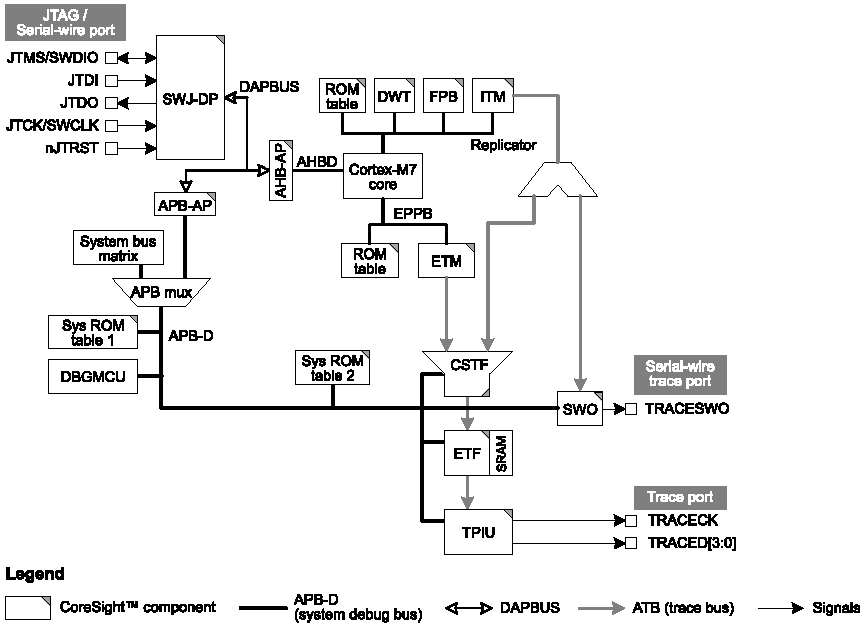
\includegraphics[width=\linewidth]{stm32h7rs_debug_infrastructure.pdf}
    \caption[Debug and trace infrastructure of the target]{Debug and trace infrastructure of the target, adapted from \cite{rm0477}}
    \label{fig:target_debug}
\end{figure}

\subsection{Development Board: NUCLEO-H7S3L8}
\label{subsec:board}
The microcontroller is used on a NUCLEO-H7S3L8. It exposes a MIPI20 connector for external debug tools, which carries the serial wire and JTAG signals together with a four-bit trace port \cite{um3276}.

\subsection{Debug Probe: STLINK-V3EC}
\label{subsec:probe}
The probe is the STLINK-V3EC embedded on the board, which supports both SWD and JTAG \cite{um3276}. It connects to the host through a USB Type-C connector and additionally provides a virtual COM port (VCP) and mass storage programming.

\subsection{Trace Resources Available on the Target}
\label{subsec:trace_resources}

\begin{table}[H]
    \centering
    \caption{Trace components of the target device}
    \label{tab:trace_resources}
    \begin{tabularx}{\linewidth}{| @{}>{\hsize=0.55\hsize\bfseries}Y | >{\hsize=0.8\hsize}Y | >{\hsize=1.65\hsize}Y@{} |}
        \hline
        Name & \textbf{Base address} & \textbf{Note} \\
        \hline
        ETM & 0xE0041000 & Implementation of the Cortex-M7 ETM, configured for instruction trace only \cite{etm_m7_trm}. \\
        \hline
        TMC & 0xE00F4000 & ETF configuration, providing two kilobytes of memory. \\
        \hline
        TPIU & 0xE00F5000 & - \\
        \hline
        Funnel & 0xE00F3000 & Funnels the ETM trace data into the TMC. It also carries the stream of the instrumentation macrocell \cite{rm0477}, which this work does not use. \\
        \hline
    \end{tabularx}
\end{table}

\section{Software Environment}
\label{sec:software}

\subsection{Development Environment}
\label{subsec:devenv}

\begin{table}[H]
    \centering
    \caption{Development environment}
    \label{tab:devenv}
    \begin{tabularx}{\linewidth}{| @{}>{\hsize=0.85\hsize\bfseries}Y | >{\hsize=1.15\hsize}Y@{} |}
        \hline
        Element & \textbf{Choice} \\
        \hline
        Host platforms & Linux and Windows \\
        \hline
        Backend language & C++23 \\
        \hline
        Frontend language & TypeScript \\
        \hline
        Compiler & Clang \\
        \hline
        Build system & CMake, Ninja generator \\
        \hline
        Frontend bundler & esbuild \\
        \hline
        Editor & Visual Studio Code \\
        \hline
    \end{tabularx}
\end{table}

\subsection{External Software Components}
\label{subsec:extsw}

\begin{table}[H]
    \centering
    \caption{External software components}
    \label{tab:software}
    \begin{tabularx}{\linewidth}{| @{}>{\hsize=0.65\hsize\bfseries}Y | >{\hsize=0.4\hsize}Y | >{\hsize=1.45\hsize}Y | >{\hsize=1.5\hsize}Y@{} |}
        \hline
        Component & \textbf{Version} & \textbf{Description} & \textbf{Justification} \\
        \hline
        OpenOCD & Fork of 0.12.0 & Open-source on-chip debugger \cite{openocd}. & Supplies the groundwork the trace drivers extend. \\
        \hline
        LLVM & 22 & Compiler infrastructure and debugger, of which the machine code layer \cite{llvm_mc} and the debugger \cite{lldb} are used. & Supplies the core debug functionality and the analysis of the program image. \\
        \hline
        OpenCSD & 1.8.3 & Library for decoding CoreSight trace \cite{opencsd}. & Simplifies the trace decoding process. \\
        \hline
        Xerces-C & 3.2.4 & XML parser. & Reads the CMSIS-SVD device descriptions. \\
        \hline
        CodeSynthesis XSD & 4.2.0 & Generator of C++ bindings from an XML schema. & Avoids writing the CMSIS-SVD bindings by hand. \\
        \hline
        Visual Studio Code & 1.125 & Editor hosting the frontend extension. & Already implements the client side of the Debug Adapter Protocol. \\
        \hline
    \end{tabularx}
\end{table}

\section{Conclusion}
This chapter has stated the three deliverables of the project, the requirements derived from them, and the environment in which they were produced. Two facts from it govern everything that follows.

The first is the hardware. The target implements both routes by which trace leaves a processor, and the bench can use only one of them, since the probe available cannot capture a trace port. The on-chip sink is therefore the route the work takes, and its capacity of two kilobytes is the constraint against which the results are read.

The second is the requirement set. The functional requirements describe a pipeline running from the configuration of a trace unit to the display of an executed source line, and the non-functional requirements constrain it to hardware already present and to an existing development tool. Chapter \ref{ch:architecture} describes the structure built to satisfy them.

        \clearpage

        \chapter{Architecture \& Implementation}
\chaplabel{ch:arch_n_impl}

\section*{Introduction}
This chapter presents the design of the solution and the implementation that realizes it. It opens with the scope of the three deliverables, the requirements derived from that scope, and the order in which the work was built. It then presents the application note and the instruction trace pipeline, which is the contribution of the project. It continues with the architecture of the engine that carries the pipeline together with the conventional debug operations. The implementation follows in three sections: the on-chip debugger, the source-level debugging, and the frontend that presents the result inside an existing development tool. The chapter closes with the supported host platforms and the provenance of the parts.

\section{Scope of the Deliverables}
\label{subsec:scope}

Each deliverable is scoped to its purpose. The application note documents the hardware, so it reaches across every STM32 family that carries the trace unit. The proof of concept only has to establish feasibility, so it is held to the smallest configuration that proves it. The debugger has to serve daily work, so it carries the conventional debug operations alongside trace. Table \ref{tab:scope} states where each boundary falls.

\begin{table}[H]
    \centering
    \caption{Scope of the three deliverables}
    \label{tab:scope}
    \begin{tabularx}{\linewidth}{| @{}>{\hsize=0.6\hsize\bfseries}Y | >{\hsize=1.4\hsize}Y@{} |}
        \hline
        Deliverable & \textbf{Scope} \\
        \hline
        \multirow{3}{*}{Application note} & Instruction trace infrastructure of every STM32 family that implements it \\
        \cline{2-2}
        & Keil \textmu Vision with the ULINKpro probe \\
        \cline{2-2}
        & IAR Embedded Workbench with the I-jet Trace probe \\
        \hline
        \multirow{3}{*}{Proof of Concept} & ETMv4 implementations \\
        \cline{2-2}
        & On-chip trace sink \\
        \cline{2-2}
        & Instruction trace \\
        \hline
        \multirow{4}{*}{Debugger} & STM32 MCUs \\
        \cline{2-2}
        & Breakpoints and variable inspection \\
        \cline{2-2}
        & Peripheral inspection, memory views and disassembly \\
        \cline{2-2}
        & Instruction trace \\
        \hline
    \end{tabularx}
\end{table}

\section{Requirements Analysis}
\label{sec:requirements}

This section states the requirements the work must satisfy. It separates them into functional requirements, which state what the solution does, and non-functional requirements, which state the conditions it operates under, and it then traces each requirement to the deliverable that carries it.

\subsection{Functional Requirements}
\label{subsec:fr}

The functional requirements follow one trace from the hardware to the source line, and Table \ref{tab:fr} keeps that order. FR1 to FR7 are the trace pipeline and hold the contribution of the project. FR8 to FR13 are the conventional debug operations, present so that trace joins a working debugger. FR7 keeps a gap in the capture visible in the record, which the trace data model and the frontend must both honor later.

\begin{table}[H]
    \centering
    \caption{Functional requirements}
    \label{tab:fr}
    \begin{tabularx}{\linewidth}{| @{}>{\hsize=0.4\hsize\bfseries}Y | >{\hsize=1.6\hsize}Y@{} |}
        \hline
        ID & \textbf{Requirement} \\
        \hline
        FR1 & Configure the trace unit and the on-chip trace sink of the target through the debug connection. \\
        \hline
        FR2 & Start and stop trace capture in step with the run state of the program, without a separate command from the developer. \\
        \hline
        FR3 & Extract the captured trace over the same debug connection that carries every other debug operation. \\
        \hline
        FR4 & Decode the extracted byte stream into trace elements. \\
        \hline
        FR5 & Reconstruct the sequence of executed instructions from those elements together with the program image. \\
        \hline
        FR6 & Attribute each reconstructed instruction to a function, a source file and a line. \\
        \hline
        FR7 & Represent a discontinuity in the capture explicitly, keeping the two sides of it distinct. \\
        \hline
        FR8 & Present the reconstruction inside a development tool during a live debug session. \\
        \hline
        FR9 & Provide the run control primitives of Section \ref{sec:primitives}, namely halting, resuming, stepping, breakpoints and watchpoints. \\
        \hline
        FR10 & Read and write memory and processor registers. \\
        \hline
        FR11 & Present the registers of a peripheral by name and by field, using a description of the device. \\
        \hline
        FR12 & Provide disassembly and source-level inspection of variables. \\
        \hline
        FR13 & Reset the target and restore the debug session to a state consistent with the reset device. \\
        \hline
    \end{tabularx}
\end{table}

\subsection{Non-Functional Requirements}
\label{subsec:nfr}

The non-functional requirements are the constraints of Chapter \ref{ch:context} stated as obligations on the solution. NFR1 has the largest effect on the design, since holding the hardware to the board's own probe leaves the on-chip buffer as the only trace route. NFR2 and NFR3 bind the result to both host platforms and to an existing development tool. Table \ref{tab:nfr} states them.

\begin{table}[H]
    \centering
    \caption{Non-functional requirements}
    \label{tab:nfr}
    \begin{tabularx}{\linewidth}{| @{}>{\hsize=0.4\hsize\bfseries}Y | >{\hsize=1.6\hsize}Y@{} |}
        \hline
        ID & \textbf{Requirement} \\
        \hline
        NFR1 & Require no hardware beyond the debug probe already present on the development board, and no trace pins. \\
        \hline
        NFR2 & Operate on Windows and on Linux. \\
        \hline
        NFR3 & Integrate with existing development tools. \\
        \hline
    \end{tabularx}
\end{table}

\subsection{Traceability to Deliverables}
\label{subsec:traceability}

Traceability confirms that every requirement has a deliverable, and that the deliverables build on one another. The application note and the proof of concept rest on the same pipeline requirements, so the proof of concept demonstrates what the note describes. The debugger owns the operations that make the reconstruction usable, together with the two portability requirements. Table \ref{tab:traceability} gives the assignment.

\begin{table}[H]
    \centering
    \caption{Traceability of requirements to deliverables}
    \label{tab:traceability}
    \begin{tabularx}{\linewidth}{| @{}>{\hsize=1.2\hsize\bfseries}Y | >{\hsize=0.9\hsize}Y | >{\hsize=0.9\hsize}Y@{} |}
        \hline
        Deliverable & \textbf{Functional} & \textbf{Non-functional} \\
        \hline
        Application note & FR1 to FR5 & NFR1 \\
        \hline
        Proof of Concept & FR1 to FR8 & NFR1 \\
        \hline
        Debugger & FR8 to FR13 & NFR2, NFR3 \\
        \hline
    \end{tabularx}
\end{table}

\section{Development Methodology}
The work was built in stages, each chosen so that a part could be validated before the next depended on it. By finding that an earlier arrangement did not hold. The order followed the trace itself, from the parts that need no device to the parts only hardware can exercise.

The first stage explored the trace infrastructure and produced the application note of Section \ref{sec:appnote}. It also produced an offline tool that decoded a stored capture against a program image, which established the decoding and reconstruction stages with no device present. Beginning offline let these stages be validated against fixed data before any acquisition existed.

The second stage addressed acquisition. Obtaining a capture without manual intervention required the trace components on the device to be configured and drained, which OpenOCD did not support, so the drivers of Section \ref{subsec:drivers} were written.

The third stage integrated the pieces. The offline tool was absorbed into a debug engine and OpenOCD was linked into it, which turned a mechanism that printed a reconstructed trace into one usable during a debug session.

The fourth stage added the remaining debugger capabilities and the frontend, and it hardened the result against a real device, where the defects of Section \ref{subsec:field_issues} appeared. The fifth stage addressed portability and packaging.

Figure \ref{fig:chronology} shows the stages and their dependencies.

\begin{figure}[htbp]
    \centering
    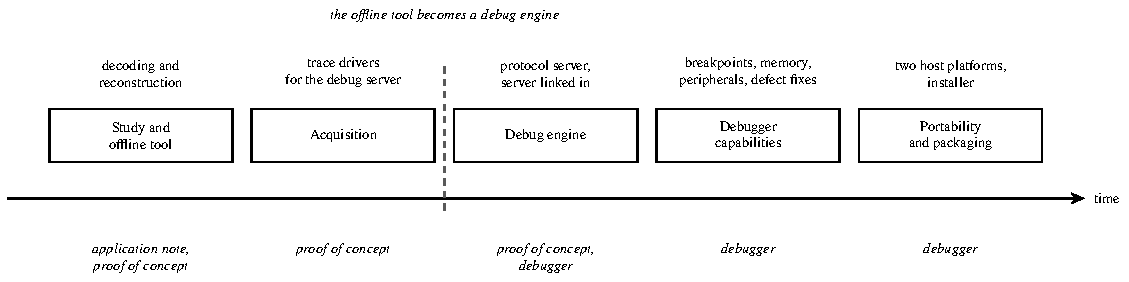
\includegraphics[width=\linewidth]{fig_chronology.pdf}
    \caption{The development methodology}
    \label{fig:chronology}
\end{figure}

\section{The Application Note}
\label{sec:appnote}
The information required to use instruction trace on these devices is correct, complete and distributed across documents written for different readers. A developer must assemble a procedure from several documents, and the assembly is the difficult part. The audience is an embedded developer who has a device, a probe and a debug session, and who wants execution history.

The first part surveys the trace infrastructure of the devices and restates in one place what the specifications and the reference manuals state separately. A reader can determine whether the trace capability is reachable with the hardware already available.

The second part walks through configuring the trace source and the trace sink, arming them, obtaining a capture, and decoding it against the program image. The difficulty of the task lies in the ordering and in the preconditions, and the walkthrough states each condition at the point where it applies.

\section{The Instruction Trace Pipeline}
\label{sec:trace_arch}
This section states the pipeline that turns the execution of a program into a record expressed in source terms. It is the primary contribution of the project.

\subsection{Pipeline Stages}
From generating the trace data on the target microcontroller to turning it into meaningful information, the pipeline is composed of four stages, the division rational is based on the functionality, the input and output of each stage. Decoupling in such an independent way allows each stage to be validated separately and is what allows offline decoding to be possible.

\begin{enumerate}[label=\arabic*.]
    \item \textbf{Generation and capture.} The trace source is configured to emit packets and the trace sink is configured to store them. Both are coupled to the run state of the processor.
    \item \textbf{Extraction.} The captured data is transferred from the on-chip buffer to the host when the processor halts.
    \item \textbf{Decoding.} The compressed byte stream is converted into trace elements.
    \item \textbf{Analysis.} Trace elements are resolved against the program image and its debug information to produce executed instructions, each attributed to a source location.
\end{enumerate}

\begin{figure}[H]
    \centering
    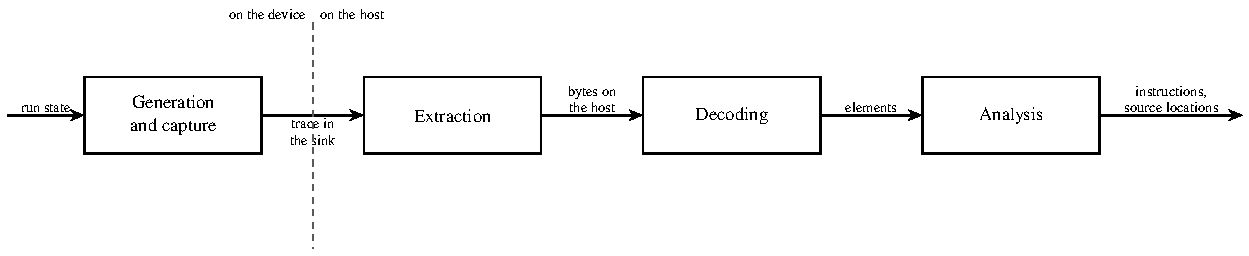
\includegraphics[width=\linewidth]{fig_pipeline.pdf}
    \caption{The four-stage instruction trace pipeline}
    \label{fig:pipeline}
\end{figure}

The implementation of this section addresses the 3 later stages, while the generation and capture stage's implementation is delegated to Section~\label{sec:trace_impl}.

\subsection{Trace Data Model}
The stages exchange value types. A reconstructed instruction records one executed instruction. A function block groups consecutive line blocks belonging to one function, and a line block groups consecutive instructions sharing one source location. A gap records a discontinuity and carries the reason for it.

\subsection{Trace Lifecycle}
\label{subsec:trace_lifecycle}
Trace progresses through four states: unavailable, idle, armed, and capturing. The diagram below shows the transitions.

The distinction between armed and capturing exists because configuration must complete before execution begins. The pipeline is prepared while the processor is halted, so that no trace is lost at the start of a run.

Each halt produces one capture. A session that resumes and halts repeatedly accumulates a sequence of captures, each appended to the record. A reset discards the entire record, because it describes a program run that no longer exists.

Two kinds of discontinuity appear in the record. A buffer overflow during a run causes the oldest data to be lost. A halt between two captures is itself a gap, since nothing is recorded while the processor is stopped.

\begin{figure}[H]
    \centering
    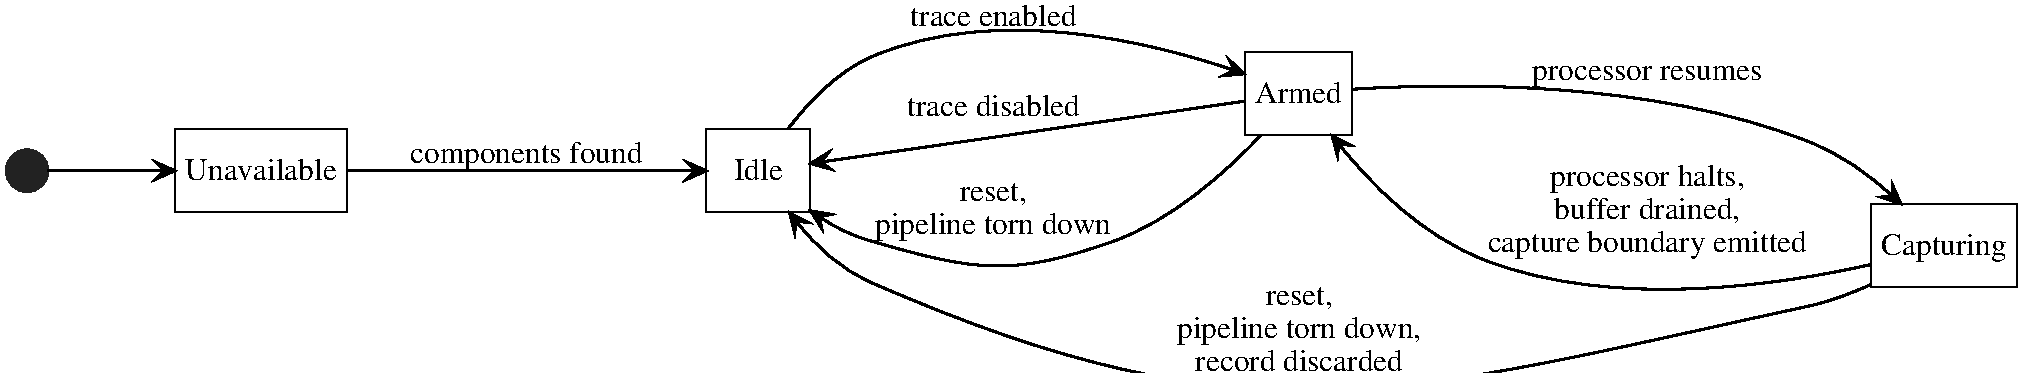
\includegraphics[width=\linewidth]{fig_trace_lifecycle.pdf}
    \caption{The trace lifecycle}
    \label{fig:trace_life}
\end{figure}

\subsection{Decoding}
\label{subsec:decode_impl}

Decoding is performed by OpenCSD. The implementation consists of configuring it correctly for each capture.

A decode tree is constructed for each block, setting up frame formatting, memory alignment, and resets on full sync frames.

The decoder must be configured exactly as the trace unit was. The identification registers are read from the unit itself, so the decoder is configured against the capabilities the hardware reports. The control register and the trace identifier hold the values the driver committed.

The program image is registered with the decoder as the source of instruction bytes, described by its loadable segments.

The decoder reports elements to a sink record object. The sink retains instruction ranges, exception and exception return elements, trace-on elements and loss-of-synchronization elements, as well as the byte offset within the captured buffer, and the trace identifier of the stream.

\begin{figure}[htbp]
    \centering
    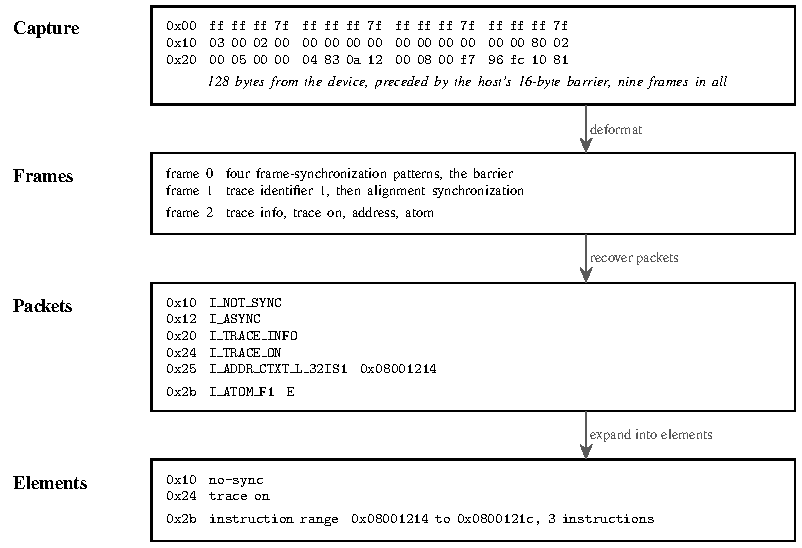
\includegraphics[width=0.92\linewidth]{fig_bytes_to_elements.pdf}
    \caption[From bytes to elements]{From bytes to elements, on the capture held as test data}
    \label{fig:bytes_to_elements}
\end{figure}


\subsection{Static Program Analysis}

The program image is opened as an ELF object file via LLVM, and its loadable segments are extracted, and registered with the decoder.

The mapping symbols partition the image into marker spans, skipping data markers to prevent literal pools from being decoded as instructions. And treating sections with no mapping symbols as a single span of the default instruction set.

Each span is decoded instruction by instruction. For every instruction the analysis records its address, length, raw bytes, mnemonic, operands and a classification: branch, call, return, conditional or indirect. When a branch target is determinable from the instruction, it is recorded. LLVM's analysis facility does not recognize the instruction forms Thumb2 architecture emits for a return, so those forms are matched on the printed instruction.

The source location of every decoded instruction is resolved during the same pass to keep reconstruction expensive, and it is done  by requesting the whole chain of inlined frames.


\subsection{Reconstructing the Execution History}

The decoded elements are converted into the model of Section \ref{sec:trace_arch} by transformations expressed over the same record sequence.

A range is expanded by walking from its start address to its end address, taking the length of each instruction from the precomputed table. When the decoder reports that the last instruction of a range was not executed, the transformation marks it and keeps it. The instruction is dropped one layer higher, when the increment is assembled, so the output of the transformation remains a complete account of what the decoder reported.

Consecutive executed instructions sharing an identical chain of source locations are merged into a line block, and consecutive line blocks belonging to the same outermost function are merged into a function block. Comparison uses the whole inlining chain to differentiate contiguous instructions from different call chains. Grouping is chronological and performs no deduplication.

Discontinuities are detected by maintaining a running count of executed instructions and emitting a gap wherever the element stream indicates one. The causes distinguished are buffer overflow, resumption of tracing after it had stopped, and loss of synchronization.


\subsection{Result Delivery}
The result is sent to the frontend as an increment. Each message states the index at which its contents begin, followed by the instructions, function blocks and gaps the capture produced.


\section{Debugger Architecture}
\label{sec:debugger_arch}
The solution is an embedded debugging engine paired with a frontend. The engine performs every debug operation. The frontend presents the results to the developer. The two are separate programs joined by the Debug Adapter Protocol.

The alternative was a single program with the interface built in. Two programs were chosen because the result must plug into a development tool the developer already uses, and a built-in interface would bind the engine to one tool. Kept separate, the engine is reached by any frontend that speaks the Debug Adapter Protocol, and it runs without a frontend for offline work.

\begin{figure}[H]
    \centering
    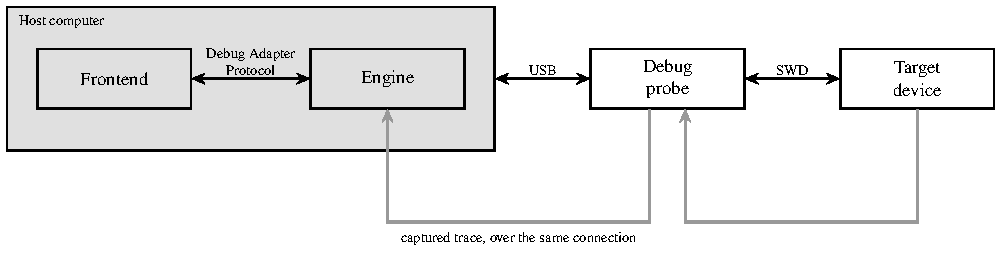
\includegraphics[width=\linewidth]{fig_global_architecture.pdf}
    \caption{Global architecture of the solution}
    \label{fig:global_arch}
\end{figure}

\subsection{Debugger Capabilities}
The engine provides the following capabilities, grouped by area.

\begin{itemize}
    \item \textbf{Run control} --- breakpoints, stepping, pause, reset
    \item \textbf{Inspection} --- variables, expressions, stack frames, disassembly
    \item \textbf{Memory} --- read, write, live observation
    \item \textbf{Peripherals} --- device description, register access, live observation
    \item \textbf{Trace} --- instruction trace capture, decoding, reconstruction, source correlation
    \item \textbf{Symbols} --- modules, source resolution
\end{itemize}

The engine is divided into six layers. Each depends only on the layers below it. The protocol types are a shared dependency used by the handlers and the context.

\begin{figure}[H]
    \centering
    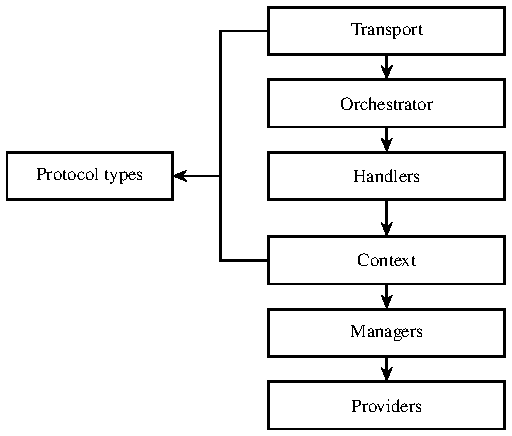
\includegraphics[width=0.6\linewidth]{fig_module_layers.pdf}
    \caption{Module dependency graph}
    \label{fig:layers}
\end{figure}

\subsection{Division of Work}
\label{subsec:division}

The engine drives two external systems that control the target device, and this section describes the responsibilities of each system.

Neither system covers the work on its own. LLDB provides source-level debugging, the DWARF and expression machinery, and stack unwinding, but it reaches the device only through GDB RSP, which offers no path to the trace components and no access to memory while the processor runs. OpenOCD reaches the debug port, the access ports and the trace components directly, but it carries no model of the program and no source-level debugging. Combining the two gives the engine both, and the responsibilities below follow from that division.

Debug primitives mentioned in Section~\ref{sec:primitives} are handled by LLDB.

The decoder requires typed register values read from hardware, and a capture arrives as a push at the moment of a halt. The engine therefore also calls OpenOCD directly through its provider.

Reading memory through LLDB requires a stopped program. A direct read through OpenOCD reaches the device while the processor runs allowing for live memory watches.

Memory access is selected when the session is established. A launched session installs the direct path through OpenOCD, and every read and write uses it. An attached session has no direct path, so trace, live memory observation and peripheral inspection are unavailable.

Reset is performed on the direct path. Section \ref{subsec:reset_impl} describes why.

\begin{figure}[H]
    \centering
    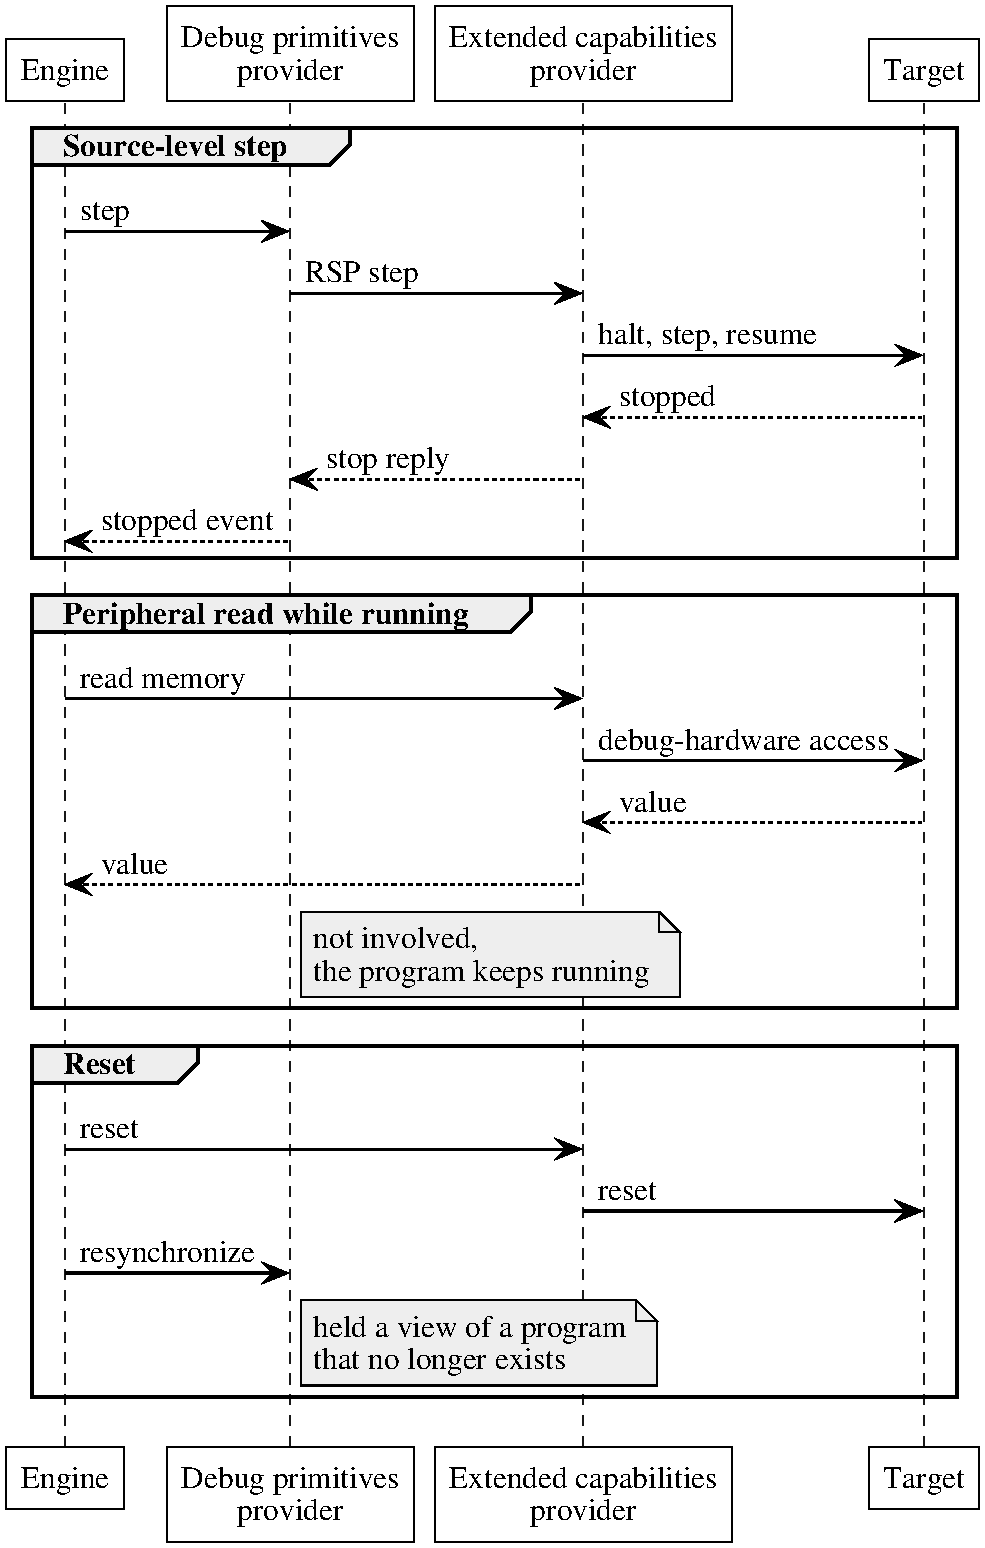
\includegraphics[width=0.62\linewidth]{fig_division_responsibility.pdf}
    \caption{Division of work between LLDB and OpenOCD}
    \label{fig:division}
\end{figure}

\subsection{Transport Layer}
The transport is the outer boundary of the engine. It reads and writes framed messages on a pair of channels. It performs no interpretation of message content. It is not bound to a particular protocol or a particular channel type.

\subsection{The Event Bus}
The event bus is a typed publish-subscribe mechanism. A producer publishes a domain event describing what happened. A single subscriber converts each domain event into a protocol message and sends it through the transport. Every producer stays free of knowledge of the wire format.

\subsection{Orchestration Layer}
The orchestrator receives messages from the transport and routes each to the handler responsible for it. It consumes events from the event bus and sends them outward through the transport. It tracks operations in progress and supports their cancellation.

\begin{figure}[H]
    \centering
    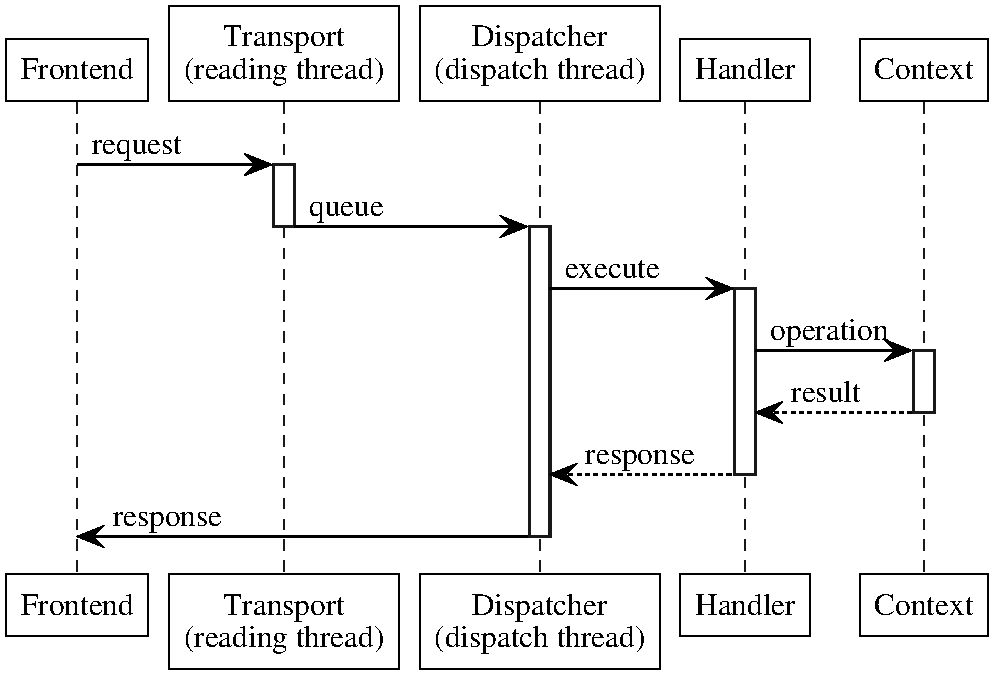
\includegraphics[width=\linewidth]{fig_request_wire_to_wire.pdf}
    \caption{Request flow from transport to response}
    \label{fig:request_flow}
\end{figure}

\subsection{Request Handlers}
The handler interface defines the contract for fulfilling a single request. A handler receives a parsed request and produces a response or an error. Handlers may respond synchronously, completing before the next request is dispatched, or asynchronously, deferring their response while the engine continues to accept other messages.

\subsection{The Debug Context}
\label{subsec:debug_context}
The debug context is a facade. It composes the event bus, the shared providers and the managers, and every handler holds a reference to it. Managers reach the shared providers and one another through it.

\begin{figure}[H]
    \centering
    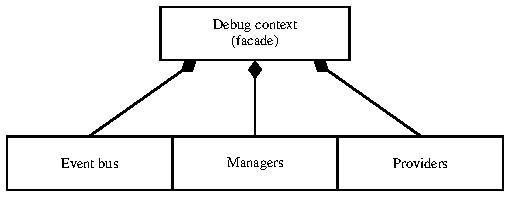
\includegraphics[width=0.85\linewidth]{fig_debug_context.pdf}
    \caption{The debug context}
    \label{fig:debug_ctx}
\end{figure}

\subsection{State Managers}
Each manager owns one area of debug state: breakpoints, memory, disassembly, modules, variables and expressions, execution control, session lifecycle, live observation, device and peripherals, and instruction trace. A manager that needs a dedicated external resource owns the provider for it. All managers use the shared providers through the debug context.

\subsection{External-System Providers}
\label{subsec:providers}
A provider adapts an external system to the needs of the engine, and no type belonging to an external system appears in any provider interface. Without this rule the types of OpenOCD, LLDB and OpenCSD would spread through the engine, and every component that touched them would depend on the library that defined them. The alternative was to let each component call those libraries directly. The abstraction was kept for three reasons. A component is tested against a substitute provider with no device and no library present. A library is replaced behind its provider without reaching the components above it. The core of the engine states its needs in its own terms and stays independent of any external interface. Five providers exist.

\begin{table}[H]
    \centering
    \caption{Provider categories}
    \label{tab:providers}
    \begin{tabularx}{\linewidth}{| @{}>{\hsize=0.55\hsize\bfseries}Y | >{\hsize=1.45\hsize}Y@{} |}
        \hline
        Provider & \textbf{Responsibility} \\
        \hline
        Debug primitives & Conventional debugging: symbol resolution, expression evaluation, stepping, stack unwinding, breakpoint management \\
        \hline
        Extended capabilities & Direct device access: memory read and write, command execution, trace component management, target state observation \\
        \hline
        Device & Device description: memory map and peripheral model \\
        \hline
        Disassembler & Static program analysis: load a program image, produce the precomputed instruction table \\
        \hline
        Trace & Trace decoding and reconstruction: accept a captured block, return the increment \\
        \hline
    \end{tabularx}
\end{table}

\subsection{Concurrency Model}
\label{subsec:concurrency}
The engine is multi-threaded. Three requirements drive the model.

\begin{itemize}
    \item A cancellation must be received while a request is being handled.
    \item Observation of memory and peripherals must continue while the program runs.
    \item The debug primitives provider does not support concurrent use.
\end{itemize}

\subsection{Session Lifecycle}

Launching creates the OpenOCD provider, installs the memory access strategy that uses it, creates the LLDB target from the program image, connects LLDB to OpenOCD's GDB RSP server, and starts the trace pipeline.

Attaching connects LLDB to a GDB RSP server the engine did not create. Every capability depending on the direct path is unavailable in this mode.

Disconnection proceeds in a fixed order. The program is detached or terminated, event handling is stopped, the trace pipeline is shut down, the observation workers are stopped, and the OpenOCD provider is destroyed last, so that no thread outlives the resource it reads from.


\subsection{Reset and Resynchronization}
\label{subsec:reset_impl}

Resetting the device is the operation where LLDB and OpenOCD conflict.

The reset is performed through the OpenOCD provider, because the reset-and-halt behavior required is not reachable through GDB RSP. The processor therefore halts without LLDB being aware meaning that its cached view of threads, frames and variables is stale.

By default, LLDB is made aware of resets via a reply to a reset request it has made, and therefore a new mechanism needs to be introduced for asynchronous device resets.

A command was added to OpenOCD that arms a synchronization flag on the GDB RSP connection. When the flag is armed, the next resume or step request received on that connection is intercepted and answered with a report of the current state. The engine arms the flag after the reset and then issues a single-instruction step through LLDB. OpenOCD intercepts the step and answers allowing LLDB to  updates its view, and the session continues against the program that is actually present.

\begin{figure}[htbp]
    \centering
    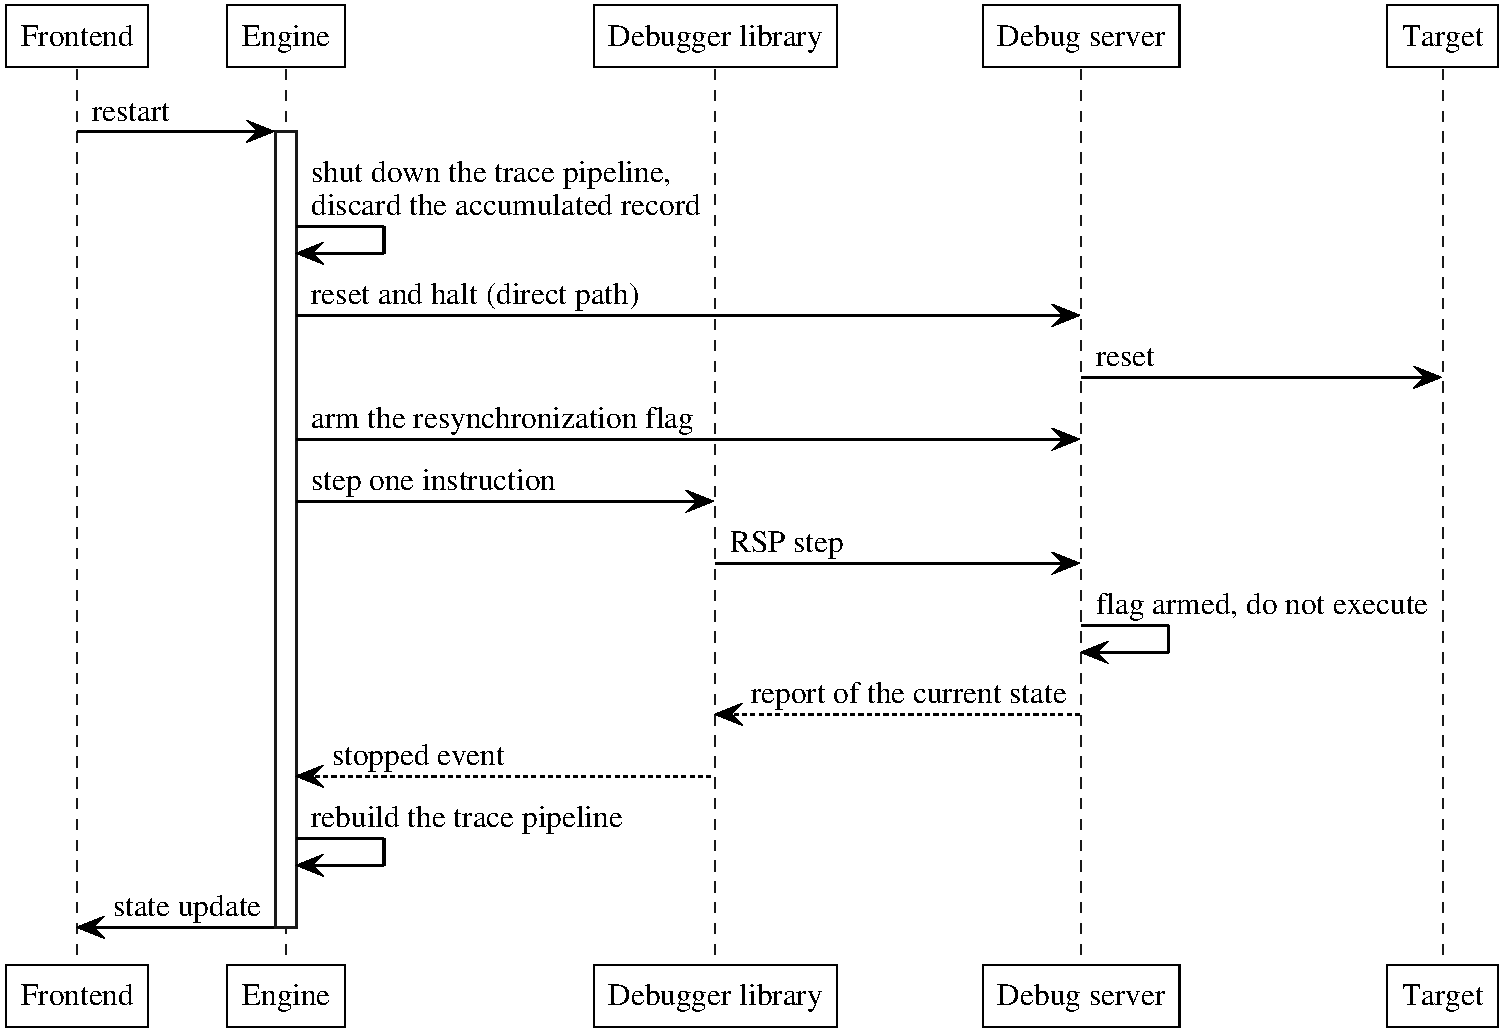
\includegraphics[width=\linewidth]{fig_reset_resync.pdf}
    \caption{Reset and resynchronization}
    \label{fig:resync}
\end{figure}



A reader thread receives messages from the transport. A dispatch thread executes them one at a time. Separating the two allows a cancellation to be recorded as soon as it arrives.

The extended capabilities provider confines its operations to a dedicated thread. Observation workers access it directly, which is what allows observation to proceed independently of request handling.

Access to the debug primitives provider is serialized. A single operation accepts a callable and runs it under a lock.

Every background thread that produces output publishes a domain event. The single subscriber converts each event into a protocol message.

\section{On-Chip Debugger: OpenOCD}
\label{sec:trace_impl}

OpenOCD is a standalone program. Making it callable from the engine required converting it into a library and adding drivers for the CoreSight components the project requires. The conversion and the two drivers are the work of this project, and OpenOCD's own debug functionality is used unchanged. This section covers them.

\subsection{Embedding as a Library}
\label{subsec:openocd_lib}

OpenOCD is designed to run as a self-contained process. Embedding it inside the engine required four changes.

\subsubsection{Build System Migration}
The original build system was replaced so that OpenOCD could be compiled as a static library consumed by the engine. Each group of source files became a CMake object library, and those groups were aggregated into a single library target with no entry point. The source file containing \texttt{main()} remains in the tree and is excluded from the build.

\subsubsection{Containing Process Termination}
OpenOCD calls \texttt{exit()} in many error paths. A library must not terminate the host process, since a failure affecting one device must not end the debug session.

Every \texttt{exit()} call was redirected to a replacement function, imposed on each translation unit by the build. The replacement checks a per-thread guard. When a guarded call is in progress, the replacement performs a non-local jump (\texttt{setjmp}/\texttt{longjmp}) back to the guard site, which returns the termination code to the caller as a failure. When no guard is active, the replacement terminates as before.

Every entry into OpenOCD from the engine is wrapped in such a guard. Destructors on the abandoned call chain are not run, and allocations are leaked. The mechanism is a containment of last resort.

\subsubsection{Embedding the Startup Scripts}
OpenOCD reads Tcl scripts from disk at startup. These scripts define much of its command surface. They are converted into byte arrays at build time and compiled into the library, removing the file-system dependency.

\subsubsection{Runtime Initialization}
The initialization that OpenOCD's \texttt{main()} would have performed is reimplemented by the engine. A command context is created, the logging subsystem is started, and each subsystem's command set is registered in the order OpenOCD requires, since later registrations depend on earlier ones.

The startup sequence then follows the order OpenOCD requires: initializing targets, the adapter and the transport, initializing the debug access port, examining the targets, initializing the flash and trace subsystems, and starting the GDB RSP server.

\subsubsection{Thread Affinity and Command Serialization}
Every OpenOCD operation executes on the thread running its server loop. That loop blocks in \texttt{select()} over sockets it owns. Work submitted from another thread must reach that thread and must wake the loop.

A service is registered with OpenOCD, bound to a port on the loopback interface, and a client socket is connected to it. Sending one byte on that connection wakes the loop. The service handler drains a queue of pending work and executes each entry. Every public method of the OpenOCD provider submits work to that queue and waits for the result, with a bounded timeout so that no caller blocks indefinitely.

\begin{figure}[htbp]
    \centering
    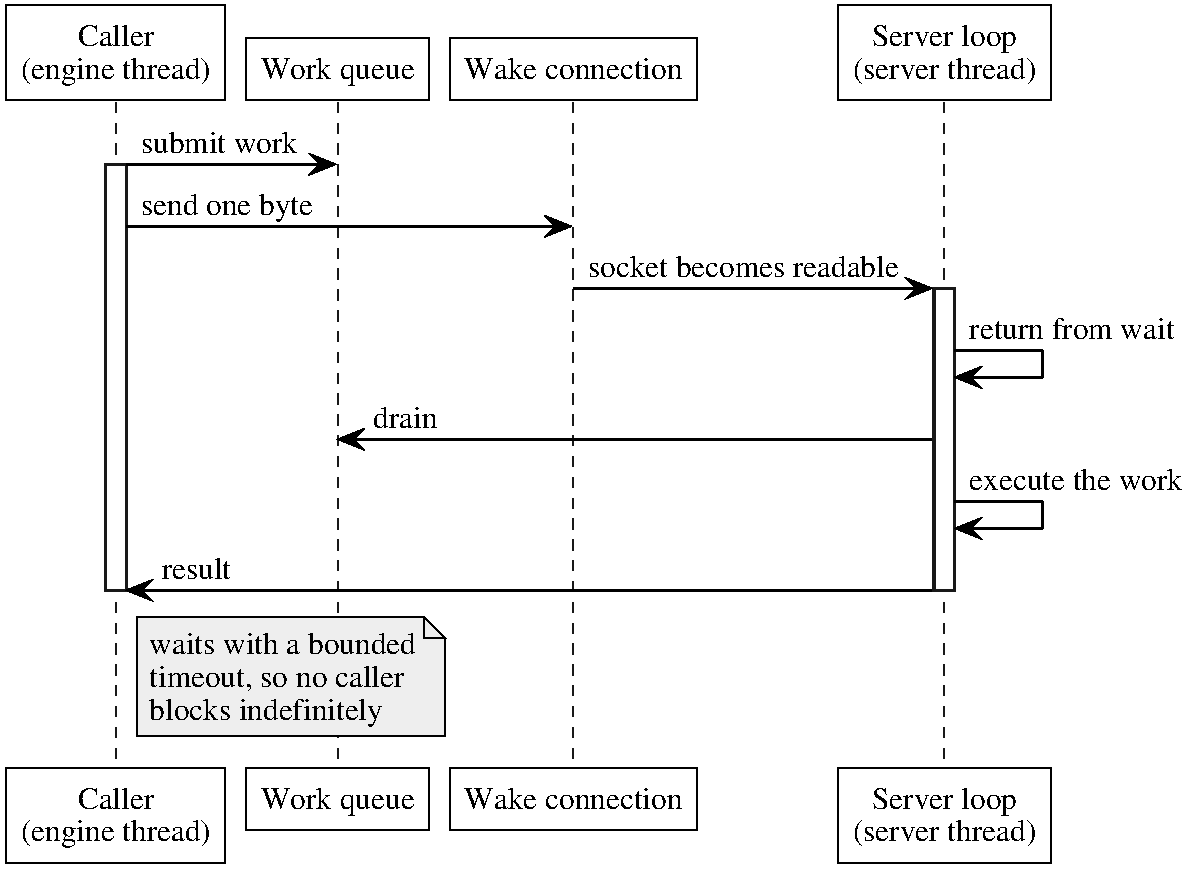
\includegraphics[width=0.8\linewidth]{fig_command_queue.pdf}
    \caption{Command queue and wake mechanism}
    \label{fig:cmdqueue}
\end{figure}

\subsection{CoreSight Drivers}
\label{subsec:drivers}

OpenOCD carries drivers for earlier CoreSight trace components but does not support the TMC or ETMv4. The two drivers were implemented as part of the project, following the patterns established by the existing CoreSight infrastructure.

Each driver is created as a named Tcl object within the OpenOCD configuration. The object exposes a \texttt{configure} command for staging options, an \texttt{init} command for hardware validation and initial setup, and \texttt{enable} and \texttt{disable} commands for requesting that trace follow the run state of the target.

\subsubsection{TMC Driver}
The driver handles all three TMC variants. The variant is determined at initialization from the DEVID and DEVTYPE registers.

The driver maintains an explicit state machine to track what the hardware is doing. Figure \ref{fig:tmc_states} shows the transitions. The state governs what operations are valid at any given moment and prevents redundant hardware access.

\begin{figure}[htbp]
    \centering
    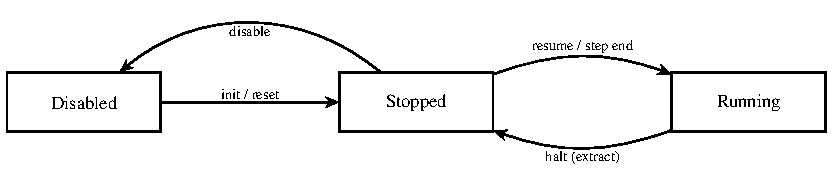
\includegraphics[width=0.7\linewidth]{fig_tmc_states.pdf}
    \caption{TMC state transitions}
    \label{fig:tmc_states}
\end{figure}

\subsubsection{ETMv4 Driver}
The ETMv4 driver adapts to the particular implementation present on the device. At initialization it reads all TRCIDR registers and decodes them into a capability structure.

First, each configuration request is validated against the discovered capabilities. Second, the driver applies capability-dependent defaults: features that must be enabled when supported are turned on, and features that may degrade gracefully are adjusted. Third, the raw identification register values are preserved as a snapshot for the trace decoder.

\subsubsection{Configuration Model}
Both drivers follow a stage-validate-commit model. Options are staged by the \texttt{configure} command, which sets dirty flags without touching hardware. When the commit path runs, it validates the staged options against the discovered identity and capabilities, then writes only the dirty registers as a batch of fixed-order, queued DAP writes. The fixed order is necessary because certain registers become meaningful only after others have been written.

\subsubsection{Run-State Coupling}
Both drivers register callbacks on target events and act on processor state transitions.

On resume, an already enabled driver validates, commits and starts the component. On halt, the ETMv4 driver stops the trace unit and the TMC driver stops capture and drains the buffer. When stepping, the ETMv4 driver starts before the step and the TMC driver starts after it, keeping the sink disarmed during single-step execution. On reset, both drivers recommit their full configuration, since the reset invalidates all register values.

Trace therefore follows the program with no host action during a run.


\subsection{Trace Extraction}
Extraction runs when the processor halts.

Capture is stopped before it is read. The driver requests that the component stop on flush, issues a manual flush, then waits for the TMCReady status bit. A component reporting an empty buffer is handled separately.

The size of the buffer to read is obtained from the CBUFLEVEL register if the component doesn't report an overflow of the buffer, otherwise, the entirety of the on-chip buffer is read. The fill level is meaningful only while capture is enabled, so capture is disabled only after the drain has completed.

The buffer is drained through TMC\_RRD, a single register that returns successive words. The read is issued as a repeated access to the register address with the automatic address increment of the access port suppressed.

The extracted block is delivered to a callback registered by the engine and, where configured, to a file or a TCP connection. A full synchronization frame is emitted ahead of every payload.

\begin{figure}[htbp]
    \centering
    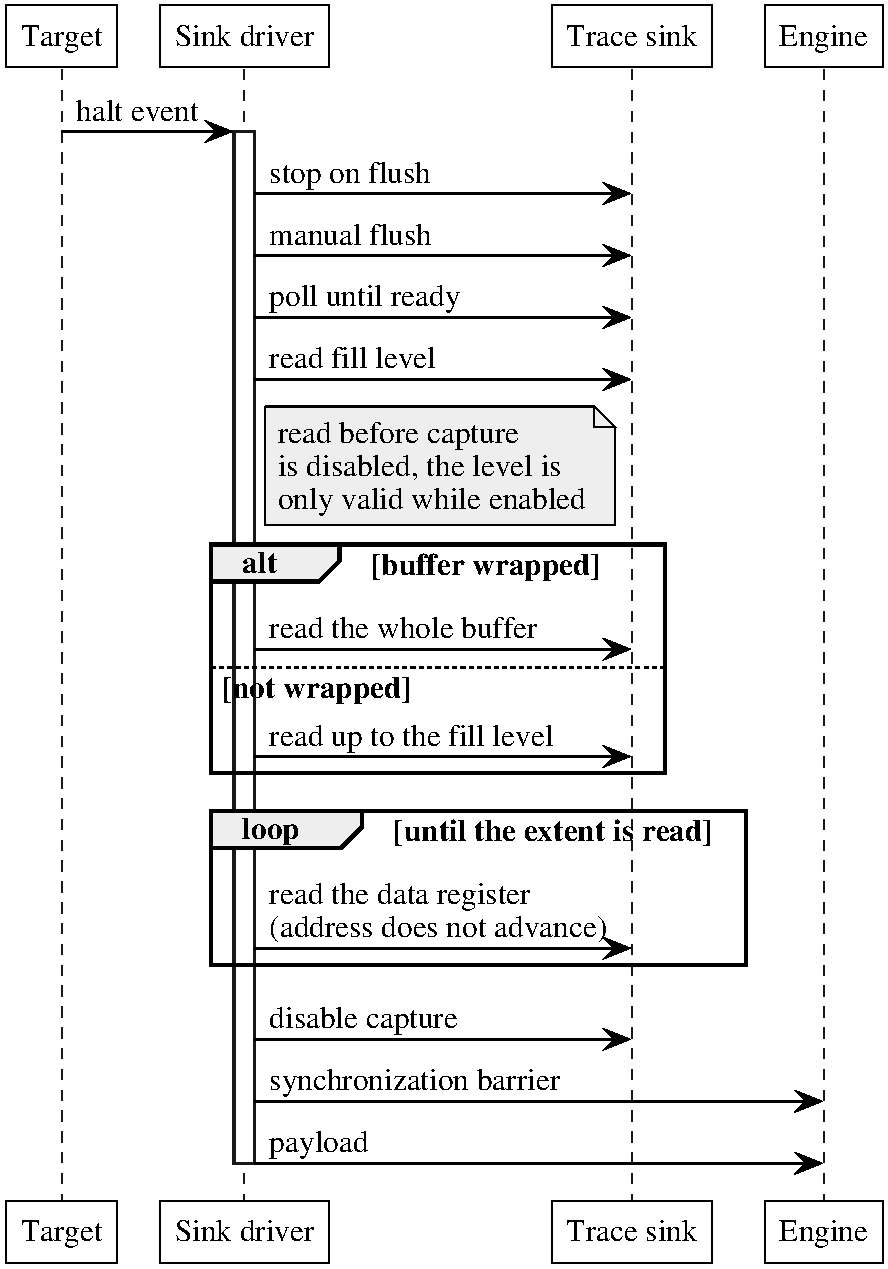
\includegraphics[width=0.55\linewidth]{fig_extraction_sequence.pdf}
    \caption{Extraction sequence}
    \label{fig:extraction}
\end{figure}

\section{Source-Level Debugging through LLDB}
\label{subsec:lldb_impl}

The engine drives LLDB through the defined LLDB SB types.

LLDB connects to the target over GDB RSP, served by OpenOCD inside the same process. The connection is made over the loopback interface.

Serialization of target access acquires the recursive API mutex of the target and invokes the supplied callable.

At startup, the following configuration elements are applied to the LLDB instance:
\begin{itemize}
    \item External symbol lookup is disabled, since LLDB otherwise attempts to fetch symbols from network services.
    \item Parallel module loading is disabled, since the background workers it creates acquire locks in an order opposite to the serialization above.
    \item The strategy for resolving breakpoints at inlined call sites is fixed, preventing a developer's personal configuration from changing where breakpoints are placed.
\end{itemize}

OpenOCD routed every GDB RSP packet beginning with a particular letter to a handler for an obsolete feature, while LLDB sends several unrelated packets beginning with that letter. OpenOCD was modified to match the complete packet name and replies to the others with the empty response that indicates an unsupported packet.

\subsection{Breakpoints}
\label{subsec:breakpoints_impl}

The choice between a software and a hardware breakpoint follows from the memory region the address lies in. The engine makes that choice automatically.

For each breakpoint the engine consults the memory map provided by the device description. If the location lies in writable memory, a software breakpoint is used. Otherwise a hardware breakpoint is used. Where no memory map is available, a hardware breakpoint is used by default.

The developer may override the decision.

\begin{figure}[htbp]
    \centering
    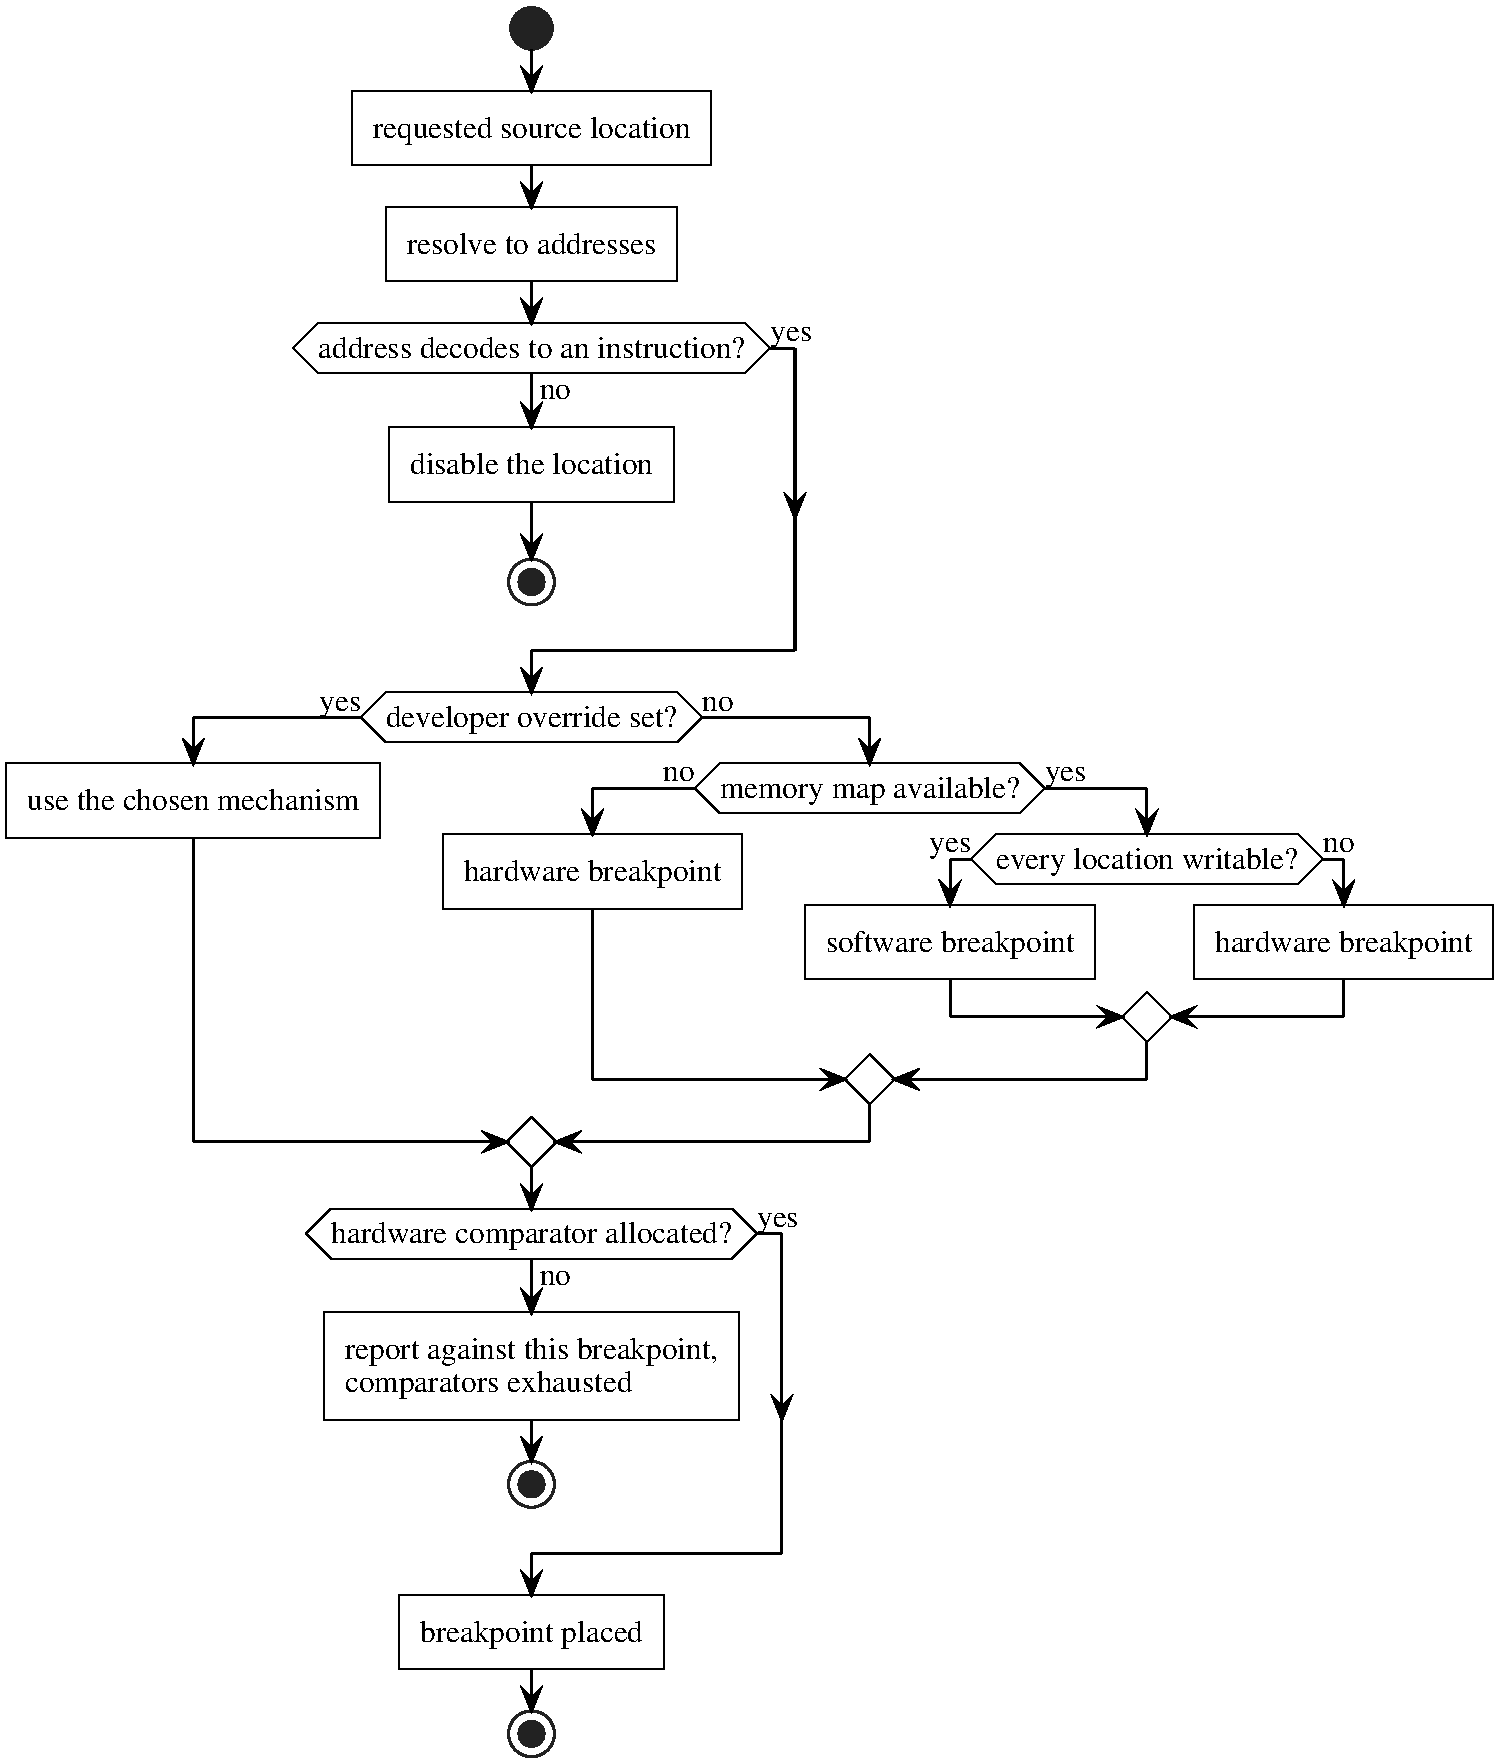
\includegraphics[width=0.62\linewidth]{fig_breakpoint_decision.pdf}
    \caption{Breakpoint placement decision}
    \label{fig:bpdecision}
\end{figure}


\subsection{Memory and Observation}

Memory is read through one of two strategies, selected when the session is established. \texttt{ProcessMemoryStrategy} reads through LLDB and serves a conventional session. \texttt{OpenOcdMemoryStrategy} reads through the OpenOCD provider and is installed whenever the direct path is available.

The second strategy does not require the program to be stopped. Live observation is built on it. Each observation runs on a dedicated thread, reads the requested region at a configured interval, and publishes the result on the event bus. The wait between reads is interruptible so that stopping an observation takes effect immediately.

Observations are not suspended while the processor is halted.


\subsection{Peripherals}
The device description is parsed from the vendor SVD file into a plain data model of peripherals, registers and fields.

A register whose reading changes the state of the peripheral is not read by default. Registers that are adjacent and safe to read are coalesced into a single access, reducing a peripheral view to a small number of reads.

A race between a write and a periodic read is resolved on the producing side. A counter is advanced whenever a write completes, and an observation whose read overlapped a completing write is discarded.

\begin{figure}[htbp]
    \centering
    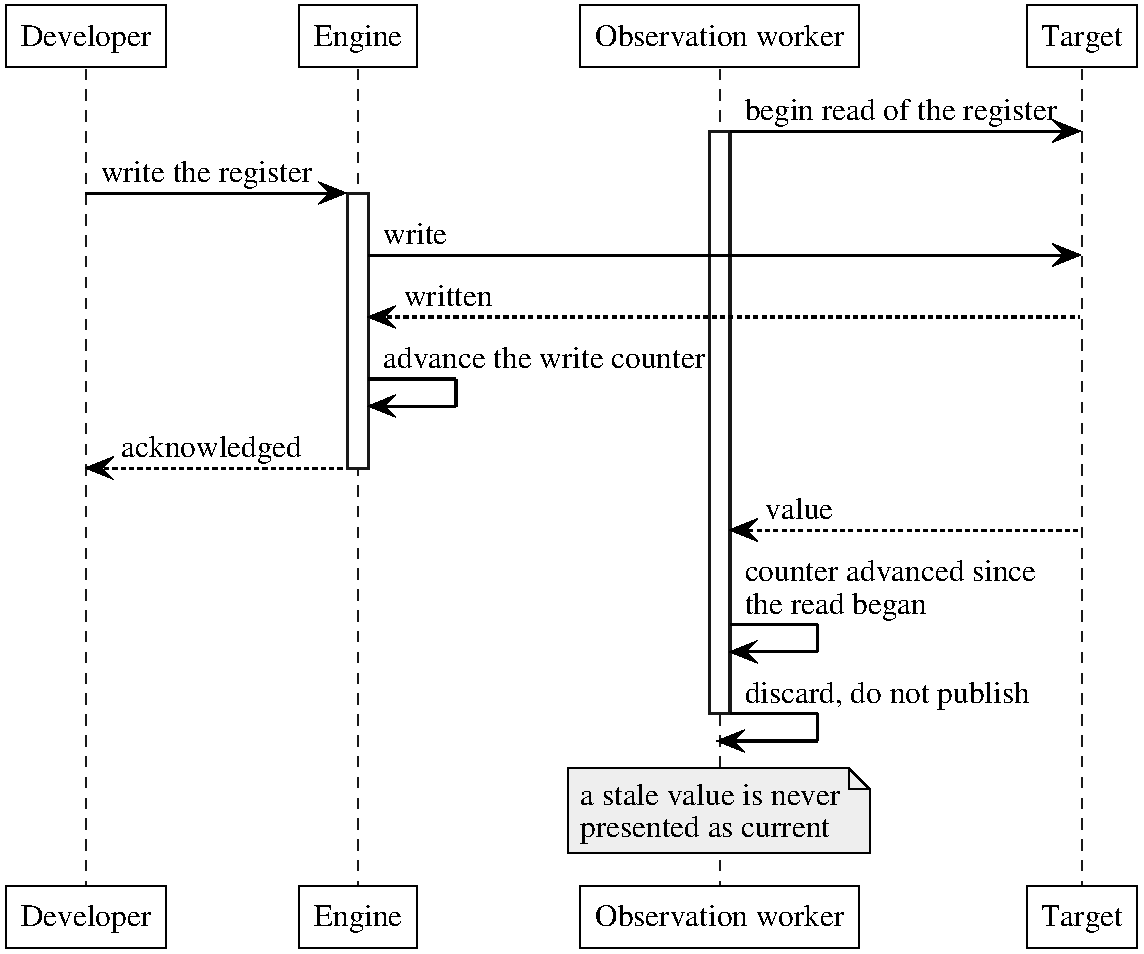
\includegraphics[width=0.8\linewidth]{fig_peripheral_race.pdf}
    \caption{Peripheral write and observation}
    \label{fig:periprace}
\end{figure}


\subsection{Variables and Expressions}
\label{subsec:boundaries}
\label{subsec:variables_impl}

Variables are obtained from LLDB. The engine converts each \texttt{SBValue} into the representation DAP defines, recursing into structured values on demand.

References to values are allocated from two spaces: one for values invalidated when the program resumes and one for values that persist. Separating them allows the first space to be cleared on every resumption without disturbing the second.

Expression evaluation is exposed through the same component. A prefix character distinguishes an expression in the source language from a command addressed to LLDB.


\section{Debugger Frontend}
The frontend is an extension for a development tool. A session object tracks which capabilities the engine advertised and enables the matching views. Each view holds a model that accumulates what the engine sends and a presentation that renders it. The engine sends increments, so the cost of an update follows the size of the change.

\subsection{Protocol Extensions}

The protocol layer implements the message framing, the dispatch and the handler hierarchy of Section \ref{sec:debugger_arch}. The engine registers a handler for each DAP request listed in Table \ref{tab:handlers}.

Handlers share a base that parses arguments, invokes the handler body and converts a returned error into an error response. Two handler shapes exist: one answering immediately and one deferring its response. The deferred shape is required by requests that must not be answered until configuration is complete.

Custom DAP requests expose embedded-specific functionality:
\begin{itemize}
    \item Trace status and control
    \item Memory observation start and stop
    \item Peripheral enumeration and access
    \item Device reset
\end{itemize}

Custom events carry what the engine produces asynchronously, trace increments, memory view values, the values of a peripheral observation, and the report that the device was reset.

\subsection{User Interface Views}
Two views present trace. One groups the record by function and line. The other lists executed instructions in order. Both render source locations as links, so selecting an entry opens the corresponding source position. Discontinuities appear as explicit separators. Chapter \ref{ch:validation} shows both views populated by a live capture.

A memory view and a set of live memory panels present regions of memory. A peripheral view presents the device description, with registers expanded to their individual fields.

\begin{figure}[H]
    \centering
    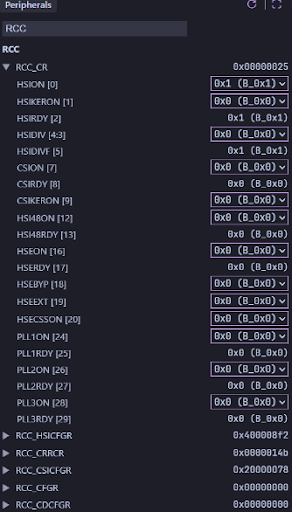
\includegraphics[width=0.85\linewidth,height=150mm,keepaspectratio]{debugger_screenshots/peripheral_view_ui.png}
    \caption[The peripheral view]{The peripheral view, with a register expanded to its individual fields.}
    \label{fig:peripheral_view}
\end{figure}

\begin{figure}[H]
    \centering
    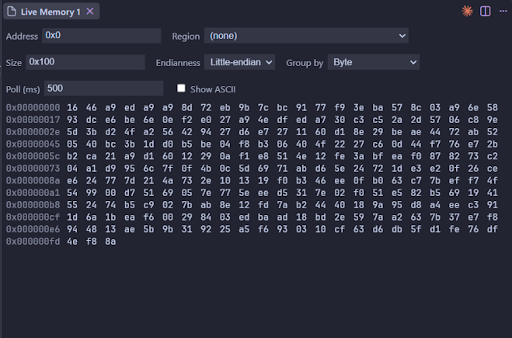
\includegraphics[width=0.85\linewidth,height=190mm,keepaspectratio]{debugger_screenshots/memory_view_ui.png}
    \caption[The live memory view]{A live memory panel.}
    \label{fig:memory_view}
\end{figure}

\section{Portability and Provenance}
The engine builds on Linux and on Windows. Portability work concentrated on protocol message reading (which requires a different mechanism on each platform), path resolution relative to the executable, and initialization requirements of the libraries used. An installer is produced for Windows, carrying the engine, its resources and the scripts of OpenOCD.

The engine is built on existing open-source work. The protocol layer began as the debug adapter distributed with LLDB and was restructured into the layers of Section \ref{sec:debugger_arch}. OpenOCD is a fork with the two CoreSight drivers and the GDB RSP corrections added. Decoding is performed by OpenCSD. Written for this project are the two CoreSight drivers, the trace pipeline from extraction through reconstruction, the domain components that constitute the core of the engine, the device description provider, and the frontend extension. The licenses of the adopted work are carried unchanged.

\section*{Conclusion}
This chapter has presented a design and its implementation. The requirements were derived from the scope of each deliverable and assigned to the deliverable that carries it. The instruction trace pipeline was presented as four stages, separated so that each stage exchanges only value types with the next. The engine that carries the pipeline was presented as a set of layers, with providers that confine each external library to one boundary and a concurrency model that keeps request handling, cancellation and observation independent of one another. The implementation converted OpenOCD into a library and added the drivers for the trace components, obtained the conventional debug operations from LLDB, and delivered the result as an extension for an existing development tool.

        \clearpage

        \chapter{Implementation}
\chaplabel{ch:implementation}

\section*{Introduction}
This chapter states how the architecture of Chapter \ref{ch:architecture} was realized. It begins with the methodology by which the work was carried out, then treats the external systems the engine embeds, the trace pipeline, the debugger and the frontend.

The engine builds on existing open-source work, and the boundary between what was adopted and what was written is stated here at the outset. OpenOCD, LLDB and OpenCSD are adopted. Written for this project are the two CoreSight drivers, the trace pipeline from extraction through reconstruction, the domain components at the core of the engine, the device description provider, and the frontend extension.

\section{Development Methodology}
The work was built in stages, each chosen so that a part could be validated before the next depended on it. Several architecture decisions of Chapter \ref{ch:architecture} were reached this way, by finding that an earlier arrangement did not hold. The order followed the trace itself, from the parts that need no device to the parts only hardware can exercise.

The first stage explored the trace infrastructure and produced the application note of Section \ref{sec:appnote}. It also produced an offline tool that decoded a stored capture against a program image, which established the decoding and reconstruction stages with no device present. Beginning offline let these stages be validated against fixed data before any acquisition existed.

The second stage addressed acquisition. Obtaining a capture without manual intervention required the trace components on the device to be configured and drained, which OpenOCD did not support, so the drivers of Section \ref{subsec:drivers} were written.

The third stage integrated the pieces. The offline tool was absorbed into a debug engine and OpenOCD was linked into it, which turned a mechanism that printed a reconstructed trace into one usable during a debug session.

The fourth stage added the remaining debugger capabilities and the frontend, and it hardened the result against a real device, where the defects of Section \ref{subsec:field_issues} appeared. The fifth stage addressed portability and packaging.

Figure \ref{fig:chronology} shows the stages and their dependencies.

\begin{figure}[htbp]
    \centering
    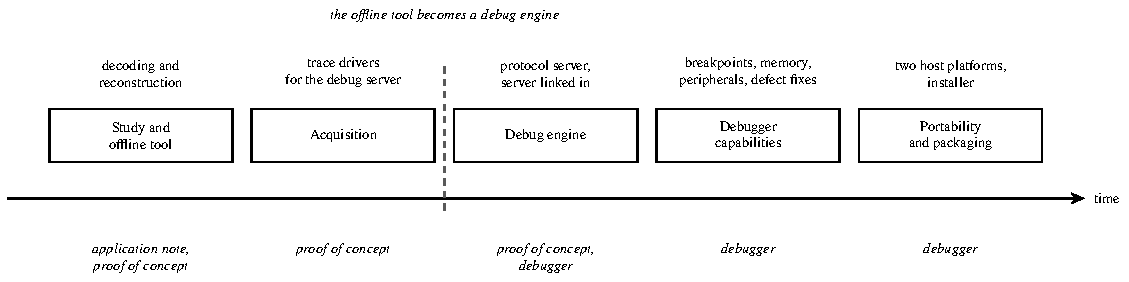
\includegraphics[width=\linewidth]{fig_chronology.pdf}
    \caption{The development methodology}
    \label{fig:chronology}
\end{figure}


\section{The Application Note}
\label{sec:appnote}
The information required to use instruction trace on these devices is correct, complete and distributed across documents written for different readers. A developer must assemble a procedure from several documents, and the assembly is the difficult part. The audience is an embedded developer who has a device, a probe and a debug session, and who wants execution history.

The first part surveys the trace infrastructure of the devices and restates in one place what the specifications and the reference manuals state separately. A reader can determine whether the trace capability is reachable with the hardware already available.

The second part walks through configuring the trace source and the trace sink, arming them, obtaining a capture, and decoding it against the program image. The difficulty of the task lies in the ordering and in the preconditions, and the walkthrough states each condition at the point where it applies.


\section{On-Chip Debugger: OpenOCD}
\label{sec:trace_impl}

OpenOCD is a standalone program. Making it callable from the engine required converting it into a library and adding drivers for the CoreSight components the project requires. The conversion and the two drivers are the work of this project, and OpenOCD's own debug functionality is used unchanged. This section covers them.

\subsection{Embedding as a Library}
\label{subsec:openocd_lib}

OpenOCD is designed to run as a self-contained process. Embedding it inside the engine required four changes.

\subsubsection{Build System Migration}
The original build system was replaced so that OpenOCD could be compiled as a static library consumed by the engine. Each group of source files became a CMake object library, and those groups were aggregated into a single library target with no entry point. The source file containing \texttt{main()} remains in the tree and is excluded from the build.

\subsubsection{Containing Process Termination}
OpenOCD calls \texttt{exit()} in many error paths. A library must not terminate the host process, since a failure affecting one device must not end the debug session.

Every \texttt{exit()} call was redirected to a replacement function, imposed on each translation unit by the build. The replacement checks a per-thread guard. When a guarded call is in progress, the replacement performs a non-local jump (\texttt{setjmp}/\texttt{longjmp}) back to the guard site, which returns the termination code to the caller as a failure. When no guard is active, the replacement terminates as before.

Every entry into OpenOCD from the engine is wrapped in such a guard. Destructors on the abandoned call chain are not run, and allocations are leaked. The mechanism is a containment of last resort.

\subsubsection{Embedding the Startup Scripts}
OpenOCD reads Tcl scripts from disk at startup. These scripts define much of its command surface. They are converted into byte arrays at build time and compiled into the library, removing the file-system dependency.

\subsubsection{Runtime Initialization}
The initialization that OpenOCD's \texttt{main()} would have performed is reimplemented by the engine. A command context is created, the logging subsystem is started, and each subsystem's command set is registered in the order OpenOCD requires, since later registrations depend on earlier ones.

The startup sequence then follows the order OpenOCD requires: initializing targets, the adapter and the transport, initializing the debug access port, examining the targets, initializing the flash and trace subsystems, and starting the GDB RSP server.

\subsubsection{Thread Affinity and Command Serialization}
Every OpenOCD operation executes on the thread running its server loop. That loop blocks in \texttt{select()} over sockets it owns. Work submitted from another thread must reach that thread and must wake the loop.

A service is registered with OpenOCD, bound to a port on the loopback interface, and a client socket is connected to it. Sending one byte on that connection wakes the loop. The service handler drains a queue of pending work and executes each entry. Every public method of the OpenOCD provider submits work to that queue and waits for the result, with a bounded timeout so that no caller blocks indefinitely.

\begin{figure}[htbp]
    \centering
    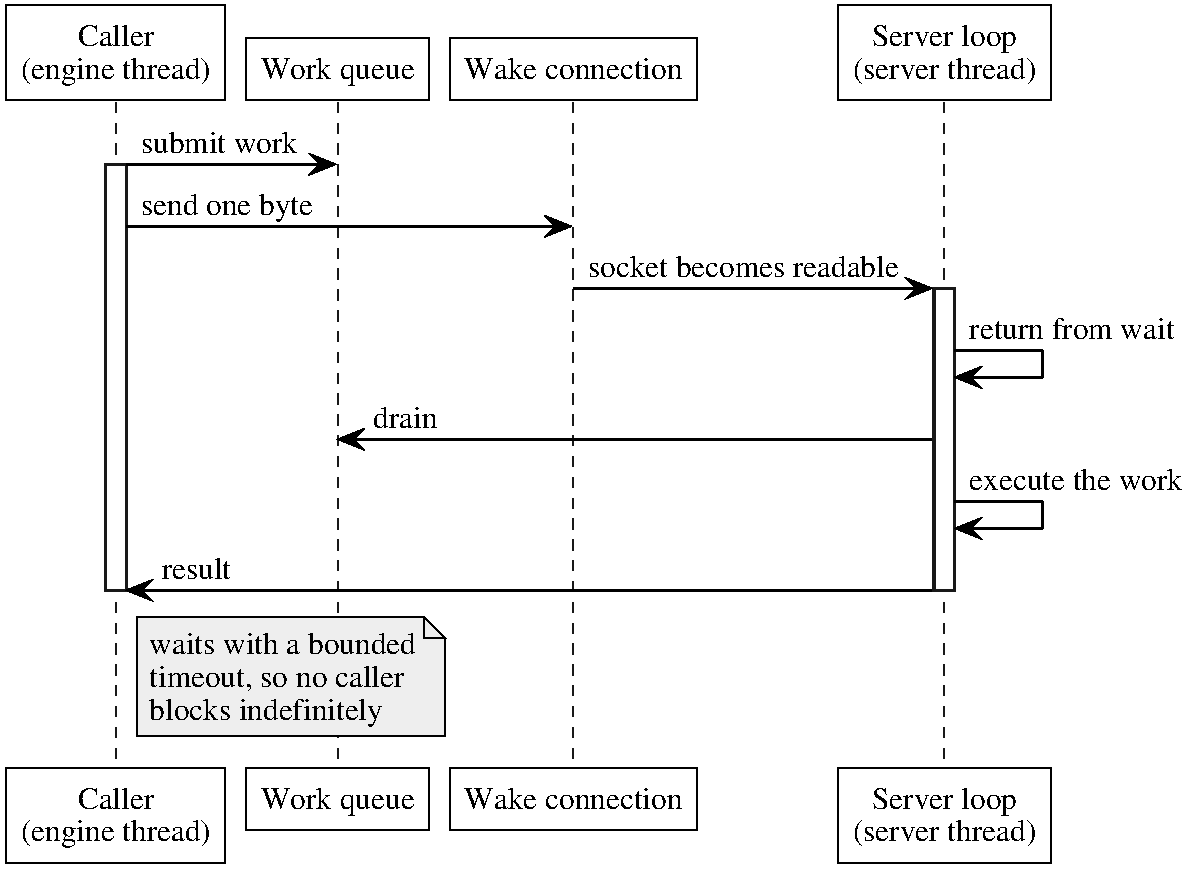
\includegraphics[width=0.8\linewidth]{fig_command_queue.pdf}
    \caption{Command queue and wake mechanism}
    \label{fig:cmdqueue}
\end{figure}

\subsection{CoreSight Drivers}
\label{subsec:drivers}

OpenOCD carries drivers for earlier CoreSight trace components but does not support the TMC or ETMv4. The two drivers were implemented as part of the project, following the patterns established by the existing CoreSight infrastructure.

Each driver is created as a named Tcl object within the OpenOCD configuration. The object exposes a \texttt{configure} command for staging options, an \texttt{init} command for hardware validation and initial setup, and \texttt{enable} and \texttt{disable} commands for requesting that trace follow the run state of the target.

\subsubsection{TMC Driver}
The driver handles all three TMC variants. The variant is determined at initialization from the DEVID and DEVTYPE registers.

The driver maintains an explicit state machine to track what the hardware is doing. Figure \ref{fig:tmc_states} shows the transitions. The state governs what operations are valid at any given moment and prevents redundant hardware access.

\begin{figure}[htbp]
    \centering
    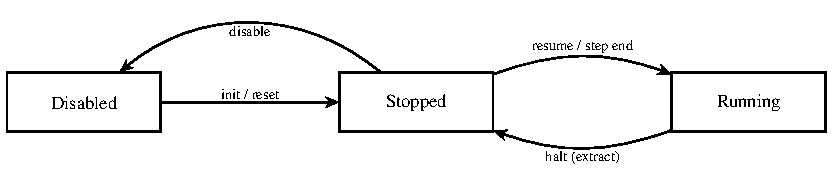
\includegraphics[width=0.7\linewidth]{fig_tmc_states.pdf}
    \caption{TMC state transitions}
    \label{fig:tmc_states}
\end{figure}

\subsubsection{ETMv4 Driver}
The ETMv4 driver adapts to the particular implementation present on the device. At initialization it reads all TRCIDR registers and decodes them into a capability structure.

First, each configuration request is validated against the discovered capabilities. Second, the driver applies capability-dependent defaults: features that must be enabled when supported are turned on, and features that may degrade gracefully are adjusted. Third, the raw identification register values are preserved as a snapshot for the trace decoder.

\subsubsection{Configuration Model}
Both drivers follow a stage-validate-commit model. Options are staged by the \texttt{configure} command, which sets dirty flags without touching hardware. When the commit path runs, it validates the staged options against the discovered identity and capabilities, then writes only the dirty registers as a batch of fixed-order, queued DAP writes. The fixed order is necessary because certain registers become meaningful only after others have been written.

\subsubsection{Run-State Coupling}
Both drivers register callbacks on target events and act on processor state transitions.

On resume, an already enabled driver validates, commits and starts the component. On halt, the ETMv4 driver stops the trace unit and the TMC driver stops capture and drains the buffer. When stepping, the ETMv4 driver starts before the step and the TMC driver starts after it, keeping the sink disarmed during single-step execution. On reset, both drivers recommit their full configuration, since the reset invalidates all register values.

Trace therefore follows the program with no host action during a run.


\subsection{Trace Extraction}
Extraction runs when the processor halts.

Capture is stopped before it is read. The driver requests that the component stop on flush, issues a manual flush, then waits for the TMCReady status bit. A component reporting an empty buffer is handled separately.

The size of the buffer to read is obtained from the CBUFLEVEL register if the component doesn't report an overflow of the buffer, otherwise, the entirety of the on-chip buffer is read. The fill level is meaningful only while capture is enabled, so capture is disabled only after the drain has completed.

The buffer is drained through TMC\_RRD, a single register that returns successive words. The read is issued as a repeated access to the register address with the automatic address increment of the access port suppressed.

The extracted block is delivered to a callback registered by the engine and, where configured, to a file or a TCP connection. A full synchronization frame is emitted ahead of every payload.

\begin{figure}[htbp]
    \centering
    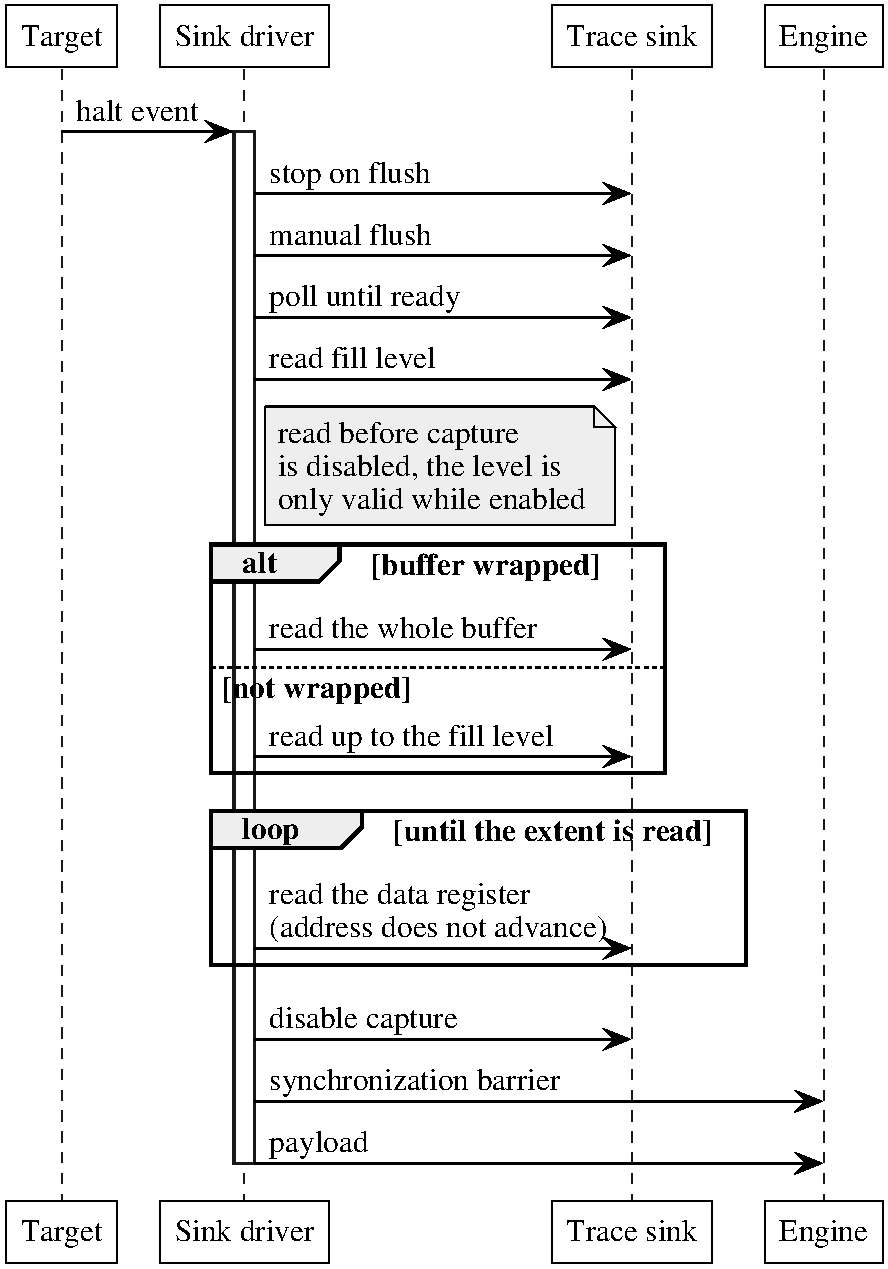
\includegraphics[width=0.55\linewidth]{fig_extraction_sequence.pdf}
    \caption{Extraction sequence}
    \label{fig:extraction}
\end{figure}


\section{Source-Level Debugging through LLDB}
\label{subsec:lldb_impl}

The engine drives LLDB through the defined LLDB SB types.

LLDB connects to the target over GDB RSP, served by OpenOCD inside the same process. The connection is made over the loopback interface.

Serialization of target access acquires the recursive API mutex of the target and invokes the supplied callable.

At startup, the following configuration elements are applied to the LLDB instance:
\begin{itemize}
    \item External symbol lookup is disabled, since LLDB otherwise attempts to fetch symbols from network services.
    \item Parallel module loading is disabled, since the background workers it creates acquire locks in an order opposite to the serialization above.
    \item The strategy for resolving breakpoints at inlined call sites is fixed, preventing a developer's personal configuration from changing where breakpoints are placed.
\end{itemize}

OpenOCD routed every GDB RSP packet beginning with a particular letter to a handler for an obsolete feature, while LLDB sends several unrelated packets beginning with that letter. OpenOCD was modified to match the complete packet name and replies to the others with the empty response that indicates an unsupported packet.


\section{Division of Work}
\label{subsec:division}

The engine drives two external systems that control the target device, and this section describes the responsibilities of each system.

Neither system covers the work on its own. LLDB provides source-level debugging, the DWARF and expression machinery, and stack unwinding, but it reaches the device only through GDB RSP, which offers no path to the trace components and no access to memory while the processor runs. OpenOCD reaches the debug port, the access ports and the trace components directly, but it carries no model of the program and no source-level debugging. Combining the two gives the engine both, and the responsibilities below follow from that division.

Debug primitives mentioned in Section~\ref{sec:primitives} are handled by LLDB.

The decoder requires typed register values read from hardware, and a capture arrives as a push at the moment of a halt. The engine therefore also calls OpenOCD directly through its provider.

Reading memory through LLDB requires a stopped program. A direct read through OpenOCD reaches the device while the processor runs allowing for live memory watches.

Memory access is selected when the session is established. A launched session installs the direct path through OpenOCD, and every read and write uses it. An attached session has no direct path, so trace, live memory observation and peripheral inspection are unavailable.

Reset is performed on the direct path. Section \ref{subsec:reset_impl} describes why.

\begin{figure}[H]
    \centering
    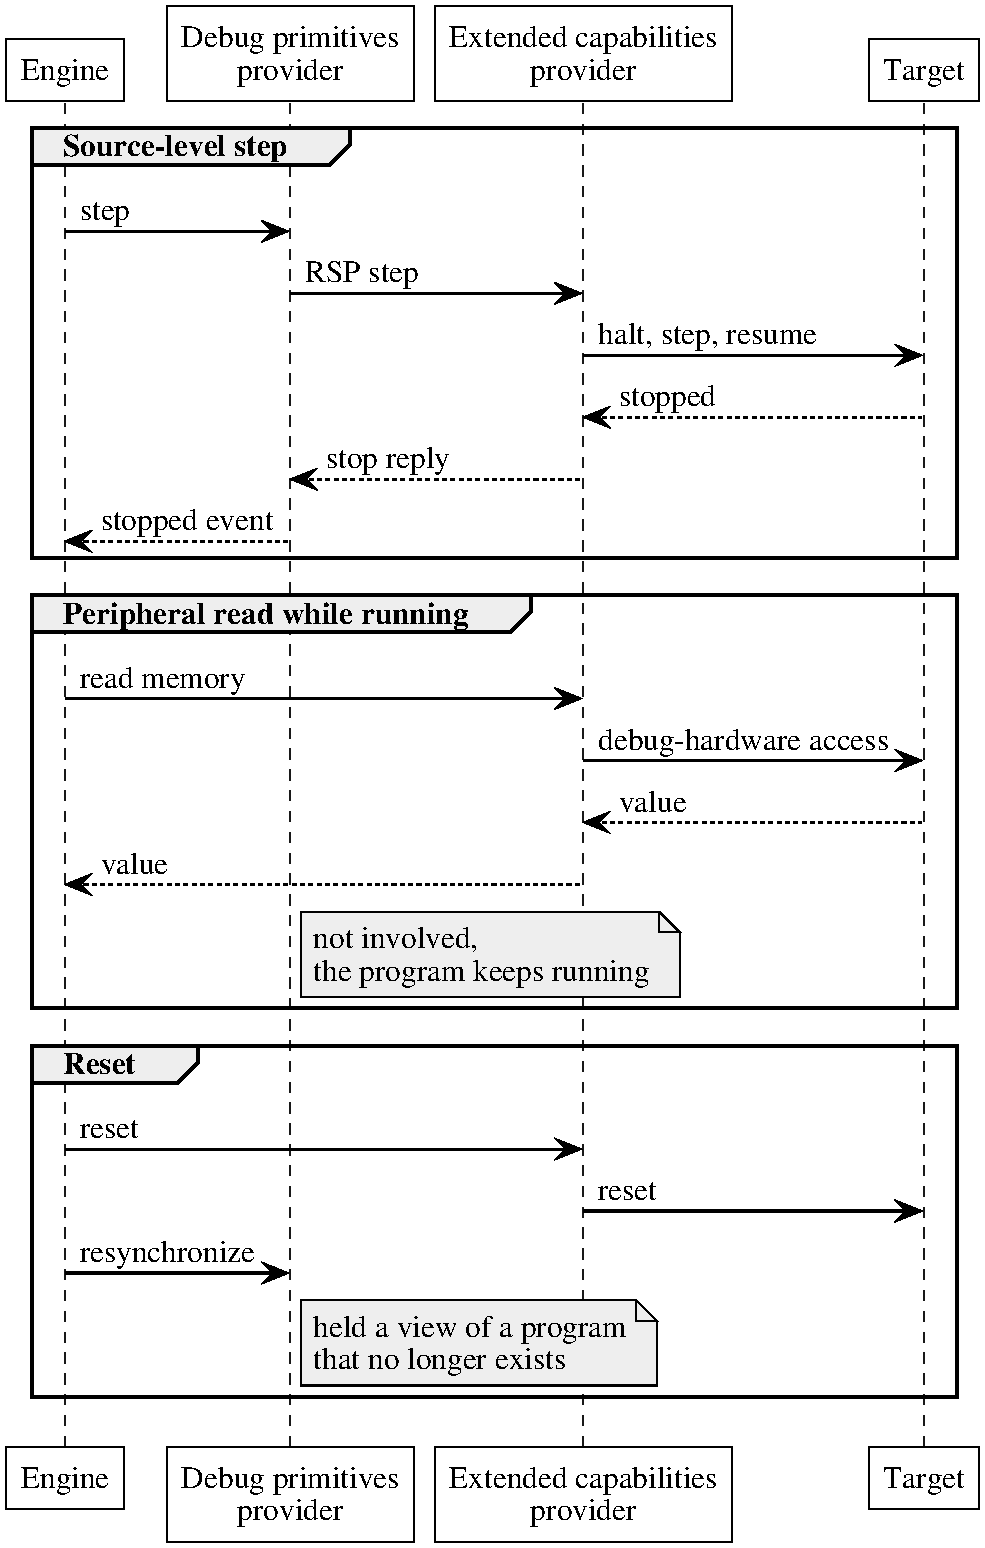
\includegraphics[width=0.62\linewidth]{fig_division_responsibility.pdf}
    \caption{Division of work between LLDB and OpenOCD}
    \label{fig:division}
\end{figure}


\section{The Trace Pipeline}

The trace pipeline operates in four stages: decoding, static program analysis, reconstruction and delivery.


\subsection{Decoding}
\label{subsec:decode_impl}

Decoding is performed by OpenCSD. The implementation consists of configuring it correctly for each capture.

A decode tree is constructed for each block, setting up frame formatting, memory alignment, and resets on full sync frames.

The decoder must be configured exactly as the trace unit was. The identification registers are read from the unit itself, so the decoder is configured against the capabilities the hardware reports. The control register and the trace identifier hold the values the driver committed.

The program image is registered with the decoder as the source of instruction bytes, described by its loadable segments.

The decoder reports elements to a sink record object. The sink retains instruction ranges, exception and exception return elements, trace-on elements and loss-of-synchronization elements, as well as the byte offset within the captured buffer, and the trace identifier of the stream.

\begin{figure}[htbp]
    \centering
    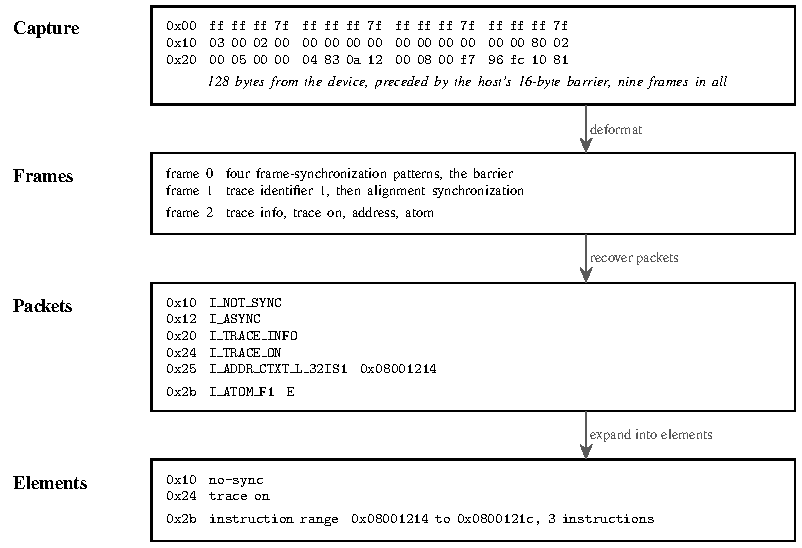
\includegraphics[width=0.92\linewidth]{fig_bytes_to_elements.pdf}
    \caption[From bytes to elements]{From bytes to elements, on the capture held as test data}
    \label{fig:bytes_to_elements}
\end{figure}


\subsection{Static Program Analysis}

The program image is opened as an ELF object file via LLVM, and its loadable segments are extracted, and registered with the decoder.

The mapping symbols partition the image into marker spans, skipping data markers to prevent literal pools from being decoded as instructions. And treating sections with no mapping symbols as a single span of the default instruction set.

Each span is decoded instruction by instruction. For every instruction the analysis records its address, length, raw bytes, mnemonic, operands and a classification: branch, call, return, conditional or indirect. When a branch target is determinable from the instruction, it is recorded. LLVM's analysis facility does not recognize the instruction forms Thumb2 architecture emits for a return, so those forms are matched on the printed instruction.

The source location of every decoded instruction is resolved during the same pass to keep reconstruction expensive, and it is done  by requesting the whole chain of inlined frames.


\subsection{Reconstruction}

The decoded elements are converted into the model of Section \ref{sec:trace_arch} by transformations expressed over the same record sequence.

A range is expanded by walking from its start address to its end address, taking the length of each instruction from the precomputed table. When the decoder reports that the last instruction of a range was not executed, the transformation marks it and keeps it. The instruction is dropped one layer higher, when the increment is assembled, so the output of the transformation remains a complete account of what the decoder reported.

Consecutive executed instructions sharing an identical chain of source locations are merged into a line block, and consecutive line blocks belonging to the same outermost function are merged into a function block. Comparison uses the whole inlining chain to differentiate contiguous instructions from different call chains. Grouping is chronological and performs no deduplication.

Discontinuities are detected by maintaining a running count of executed instructions and emitting a gap wherever the element stream indicates one. The causes distinguished are buffer overflow, resumption of tracing after it had stopped, and loss of synchronization.


\subsection{Delivery}
The result is sent to the frontend as an increment. Each message states the index at which its contents begin, followed by the instructions, function blocks and gaps the capture produced.

\section{The Debugger}
\label{sec:debugger_impl}

This section describes how the debugger is implemented on the architecture of Chapter \ref{ch:architecture}. It follows the session from its creation through the operations the developer drives, covering the session lifecycle, reset and resynchronization, breakpoints, memory and live observation, peripheral access, variables and expressions, and the extensions that carry the operations the standard protocol does not define.

\subsection{Session Lifecycle}

Launching creates the OpenOCD provider, installs the memory access strategy that uses it, creates the LLDB target from the program image, connects LLDB to OpenOCD's GDB RSP server, and starts the trace pipeline.

Attaching connects LLDB to a GDB RSP server the engine did not create. Every capability depending on the direct path is unavailable in this mode.

Disconnection proceeds in a fixed order. The program is detached or terminated, event handling is stopped, the trace pipeline is shut down, the observation workers are stopped, and the OpenOCD provider is destroyed last, so that no thread outlives the resource it reads from.


\subsection{Reset and Resynchronization}
\label{subsec:reset_impl}

Resetting the device is the operation where LLDB and OpenOCD conflict.

The reset is performed through the OpenOCD provider, because the reset-and-halt behavior required is not reachable through GDB RSP. The processor therefore halts without LLDB being aware meaning that its cached view of threads, frames and variables is stale.

By default, LLDB is made aware of resets via a reply to a reset request it has made, and therefore a new mechanism needs to be introduced for asynchronous device resets.

A command was added to OpenOCD that arms a synchronization flag on the GDB RSP connection. When the flag is armed, the next resume or step request received on that connection is intercepted and answered with a report of the current state. The engine arms the flag after the reset and then issues a single-instruction step through LLDB. OpenOCD intercepts the step and answers allowing LLDB to  updates its view, and the session continues against the program that is actually present.

\begin{figure}[htbp]
    \centering
    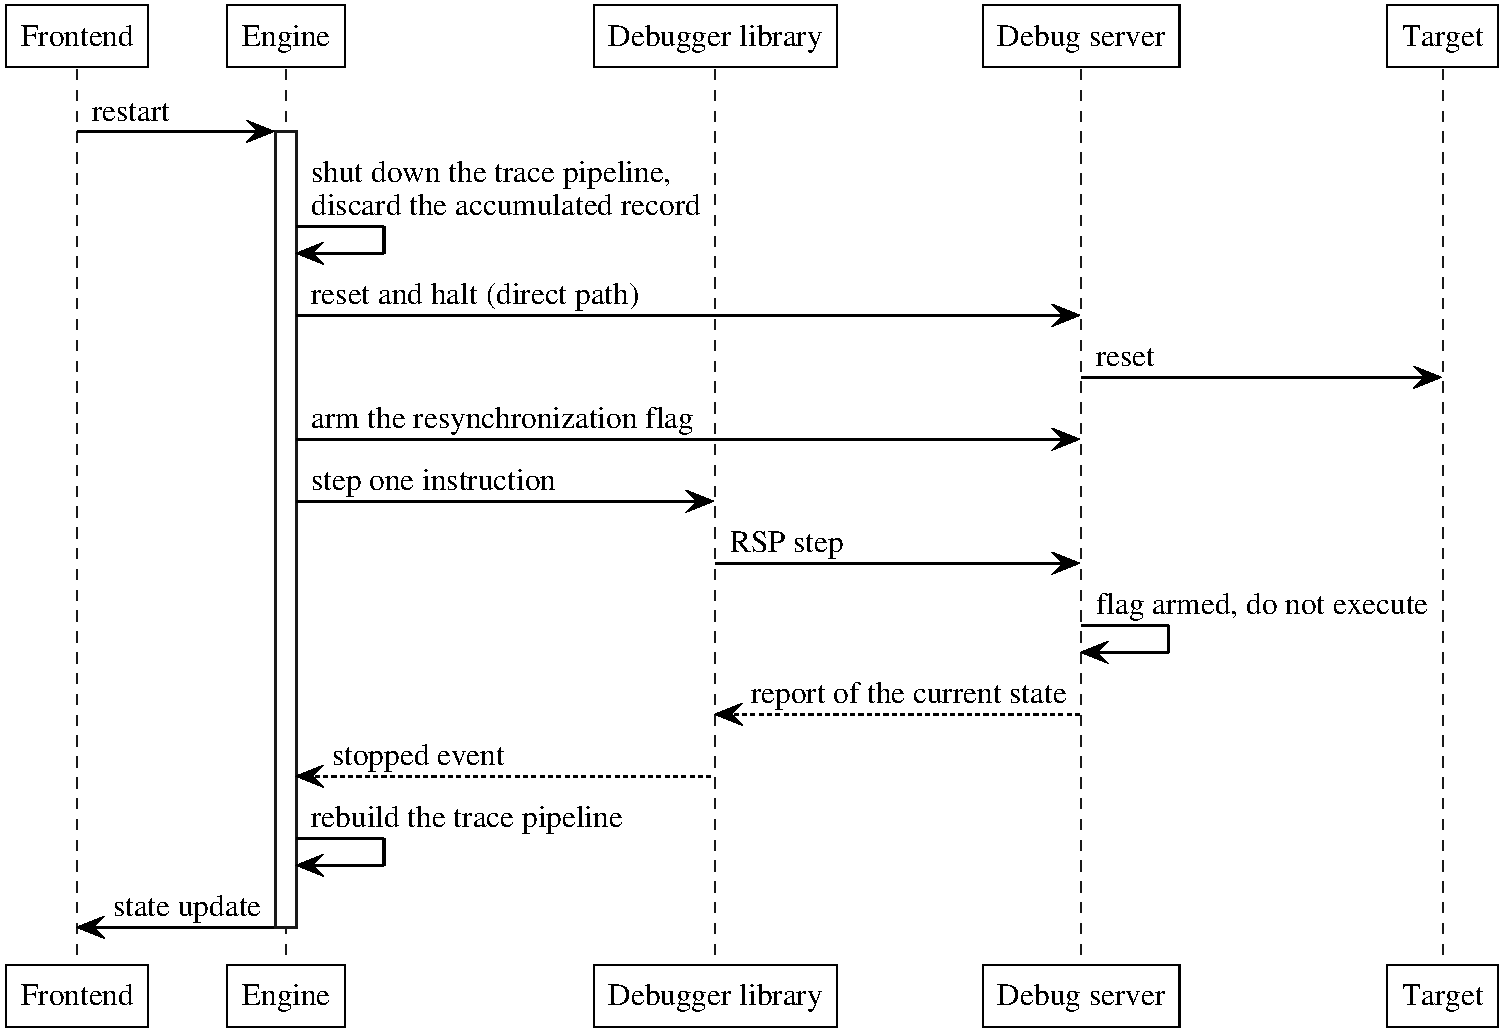
\includegraphics[width=\linewidth]{fig_reset_resync.pdf}
    \caption{Reset and resynchronization}
    \label{fig:resync}
\end{figure}


\subsection{Breakpoints}
\label{subsec:breakpoints_impl}

The choice between a software and a hardware breakpoint follows from the memory region the address lies in. The engine makes that choice automatically.

For each breakpoint the engine consults the memory map provided by the device description. If the location lies in writable memory, a software breakpoint is used. Otherwise a hardware breakpoint is used. Where no memory map is available, a hardware breakpoint is used by default.

The developer may override the decision.

\begin{figure}[htbp]
    \centering
    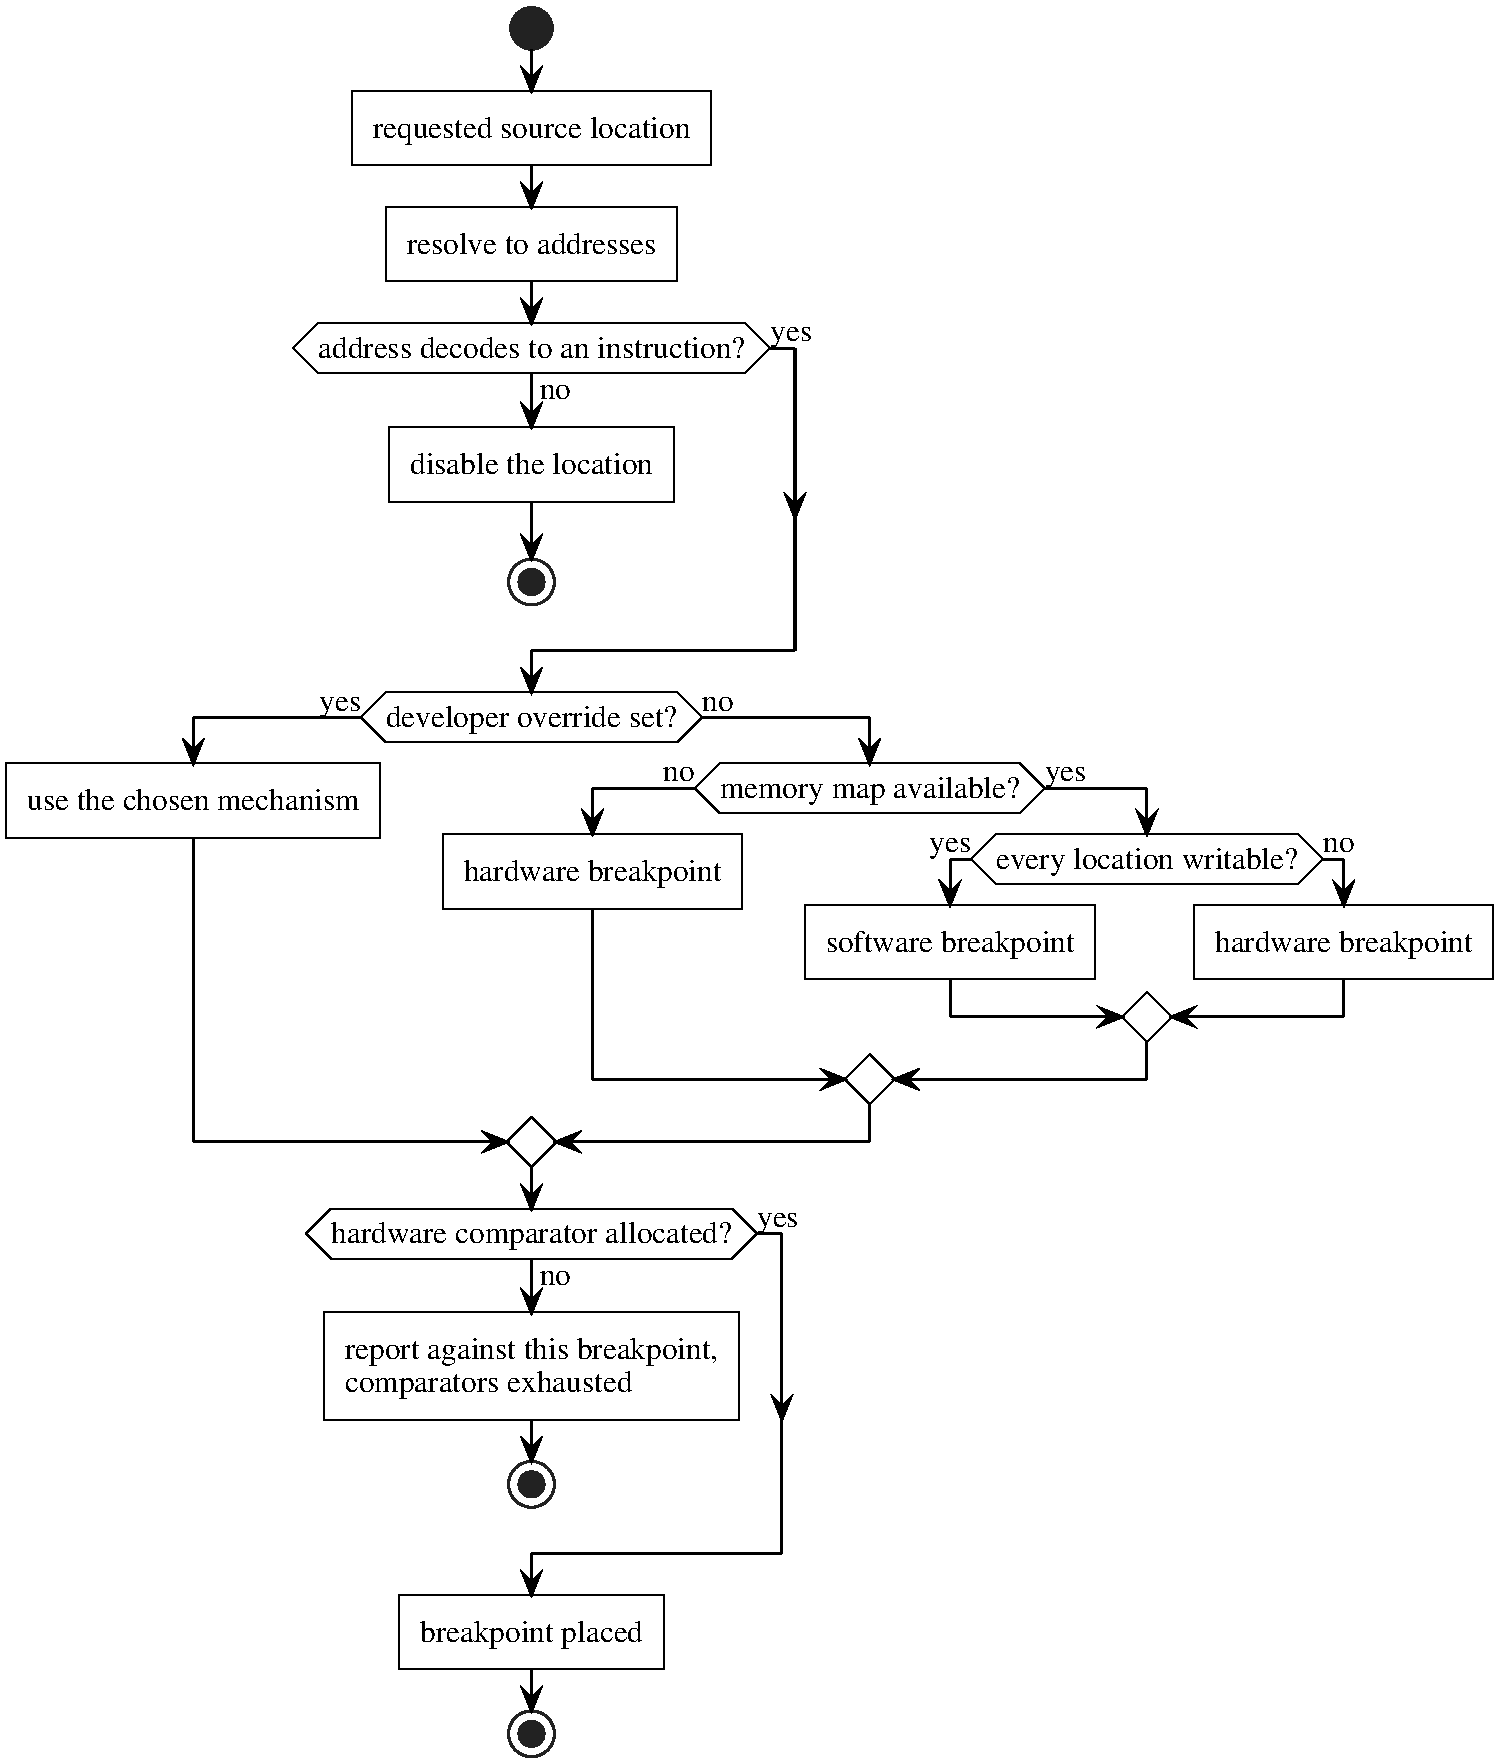
\includegraphics[width=0.62\linewidth]{fig_breakpoint_decision.pdf}
    \caption{Breakpoint placement decision}
    \label{fig:bpdecision}
\end{figure}


\subsection{Memory and Observation}

Memory is read through one of two strategies, selected when the session is established. \texttt{ProcessMemoryStrategy} reads through LLDB and serves a conventional session. \texttt{OpenOcdMemoryStrategy} reads through the OpenOCD provider and is installed whenever the direct path is available.

The second strategy does not require the program to be stopped. Live observation is built on it. Each observation runs on a dedicated thread, reads the requested region at a configured interval, and publishes the result on the event bus. The wait between reads is interruptible so that stopping an observation takes effect immediately.

Observations are not suspended while the processor is halted.


\subsection{Peripherals}
The device description is parsed from the vendor SVD file into a plain data model of peripherals, registers and fields.

A register whose reading changes the state of the peripheral is not read by default. Registers that are adjacent and safe to read are coalesced into a single access, reducing a peripheral view to a small number of reads.

A race between a write and a periodic read is resolved on the producing side. A counter is advanced whenever a write completes, and an observation whose read overlapped a completing write is discarded.

\begin{figure}[htbp]
    \centering
    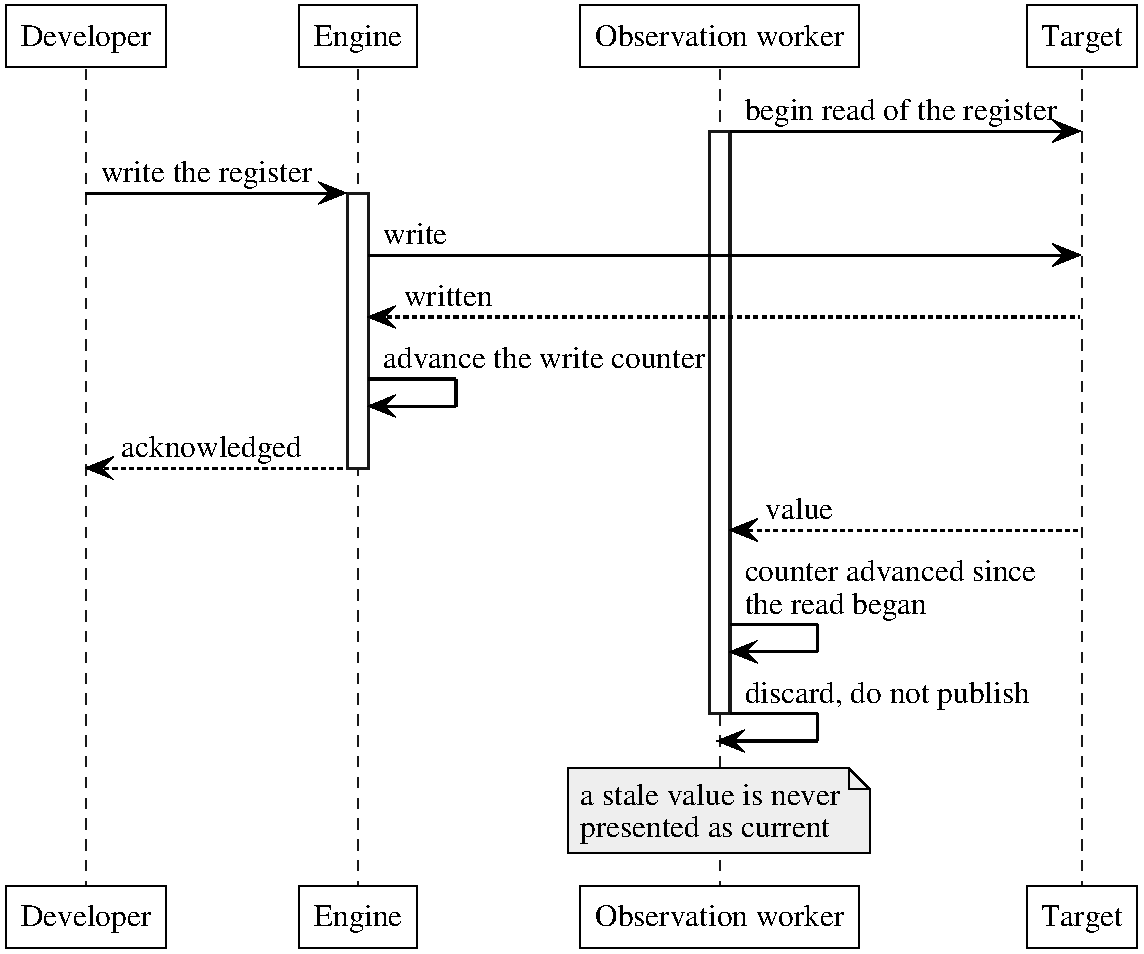
\includegraphics[width=0.8\linewidth]{fig_peripheral_race.pdf}
    \caption{Peripheral write and observation}
    \label{fig:periprace}
\end{figure}


\subsection{Variables and Expressions}
\label{subsec:boundaries}
\label{subsec:variables_impl}

Variables are obtained from LLDB. The engine converts each \texttt{SBValue} into the representation DAP defines, recursing into structured values on demand.

References to values are allocated from two spaces: one for values invalidated when the program resumes and one for values that persist. Separating them allows the first space to be cleared on every resumption without disturbing the second.

Expression evaluation is exposed through the same component. A prefix character distinguishes an expression in the source language from a command addressed to LLDB.


\subsection{Protocol Extensions}

The protocol layer implements the message framing, the dispatch and the handler hierarchy of Section \ref{sec:debugger_arch}. The engine registers a handler for each DAP request listed in Table \ref{tab:handlers}.

Handlers share a base that parses arguments, invokes the handler body and converts a returned error into an error response. Two handler shapes exist: one answering immediately and one deferring its response. The deferred shape is required by requests that must not be answered until configuration is complete.

Custom DAP requests expose embedded-specific functionality:
\begin{itemize}
    \item Trace status and control
    \item Memory observation start and stop
    \item Peripheral enumeration and access
    \item Device reset
\end{itemize}

Custom events carry what the engine produces asynchronously, trace increments, memory view values, the values of a peripheral observation, and the report that the device was reset.


\section{The Frontend}

The frontend is a VS Code extension. It contributes the views that the standard DAP protocol does not cover. The extension contains no debugger logic. It presents data received from the engine.

Two views present trace. One groups the record by function and line. The other lists executed instructions in order. Both render source locations as links, so selecting an entry opens the corresponding source position. Discontinuities appear as explicit separators. Chapter \ref{ch:validation} shows both views populated by a live capture.

A memory view and a set of live memory panels present regions of memory. A peripheral view presents the device description, with registers expanded to their individual fields.

\begin{figure}[H]
    \centering
    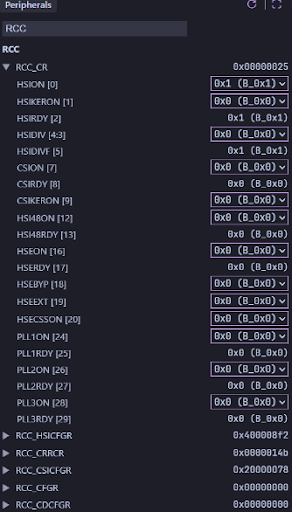
\includegraphics[width=0.85\linewidth,height=150mm,keepaspectratio]{debugger_screenshots/peripheral_view_ui.png}
    \caption[The peripheral view]{The peripheral view, with a register expanded to its individual fields.}
    \label{fig:peripheral_view}
\end{figure}

\begin{figure}[H]
    \centering
    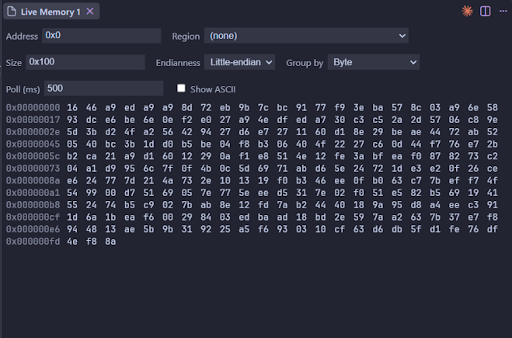
\includegraphics[width=0.85\linewidth,height=190mm,keepaspectratio]{debugger_screenshots/memory_view_ui.png}
    \caption[The live memory view]{A live memory panel.}
    \label{fig:memory_view}
\end{figure}


\subsection{Portability and Provenance}
The engine builds on Linux and on Windows. Portability work concentrated on protocol message reading (which requires a different mechanism on each platform), path resolution relative to the executable, and initialization requirements of the libraries used. An installer is produced for Windows, carrying the engine, its resources and the scripts of OpenOCD.

The engine is built on existing open-source work. The protocol layer began as the debug adapter distributed with LLDB and was restructured into the layers of Section \ref{sec:debugger_arch}. OpenOCD is a fork with the two CoreSight drivers and the GDB RSP corrections added. Decoding is performed by OpenCSD. Written for this project are the two CoreSight drivers, the trace pipeline from extraction through reconstruction, the domain components that constitute the core of the engine, the device description provider, and the frontend extension. The licenses of the adopted work are carried unchanged.


\section{Conclusion}
This chapter has described the realization of the three deliverables. The application note assembles into one document the procedure for using instruction trace on these devices. The trace pipeline configures the components on the device, extracts a capture over the ordinary debug connection, decodes it against the program image, and reconstructs the executed instructions with their source locations. The debugger makes that pipeline usable during development and supplies the conventional capabilities alongside it.

        \clearpage

        \chapter{Experimental Validation and Results}
\chaplabel{ch:validation}
\label{sec:testing}

\section*{Introduction}
The preceding chapters described the objectives set for the work, the architecture designed to meet them, and the implementation that realized it. This chapter establishes whether the result satisfies those objectives and the requirements derived from them. It states the strategy by which the engine was tested, the bench on which the tests were run, and the means by which the reconstructed trace was checked for correctness. It then reports the defects that appeared only on hardware, the results obtained against each requirement, and the limitations that remain together with the directions they suggest.


\section{Test Strategy}
Testing was organized in three tiers, distinguished by what each requires.

The first tier requires nothing beyond the built engine. It covers the protocol handshake, the cancellation path, and the components that operate on stored data: the device description parser, the static program analysis, the trace decoder and the reconstruction transformations. This tier runs during ordinary development.

The second tier requires a device. It drives the engine at the protocol level with a script that sends DAP requests and checks responses, covering launching, attaching, stepping, breakpoints, peripheral access and trace.

The third tier requires a device and the frontend. It drives the extension inside VS Code and checks the behavior a developer would observe, including that the views populate and that state is refreshed after a reset. It is exercised by hand.

No unit testing framework is used. Tests in the first tier are plain executables that return a status, keeping the build free of an additional dependency.

Concurrency is covered separately. A test publishes on the event bus from several threads at once, so that a defect in its locking appears as a detected race. The engine was additionally built with a thread sanitizer and driven against the device, which is how the lock-order inversion of Section \ref{subsec:lldb_impl} was identified. Table \ref{tab:tests} in the annexes lists the tests.


\section{Hardware Test Bench}
\label{subsec:bench}
The bench consists of a development board carrying the target device together with an on-board probe, connected to the host by a single cable. It contains no trace probe and no connection to trace pins. Every trace result reported below was obtained over the same connection used for ordinary debugging, which is the objective stated in Chapter \ref{ch:specification}.

A small firmware project serves as the program under examination, built with debug information and with the optimization settings a developer would ordinarily use.

Every result reported in this chapter was obtained in a session that the engine launched, since trace, live memory observation and peripheral inspection all depend on the direct path.

The pipeline was additionally exercised on an STM32H7 and an STM32N6, the second of which implements a different trace unit on a later processor. The base addresses and the OpenOCD configuration script changed. Neither driver was modified, since each reads the capabilities of the component it drives from that component's own identification registers.


\section{Trace Correctness Validation}
\label{subsec:trace_validation}
Correctness was checked against a stored capture, against the device, and against commercial debuggers.

The decoding and reconstruction stages are checked against a stored capture. The capture, the program image and the trace unit register values recorded from the device are held as test data. The test decodes the capture and asserts that the number of executed instructions equals a fixed expected value, that every reconstructed address corresponds to an instruction in the static analysis, and that at least one function block carries a resolved function name. Holding the register values as data allows the test to reproduce the configuration the hardware actually had.

The acquisition stages are checked against the device. A test asserts that the trace components are found, that the register values read from the trace unit match those recorded, and that a capture delivers exactly two callbacks per halt: the synchronization barrier followed by the payload.

The reconstruction was compared against the output of three commercial debuggers, each driving the probe of its own vendor. The decoded listings were compared instruction by instruction, and the sequences agreed. The differences were confined to presentation.

A capture obtained by a probe of another vendor was decoded by the same pipeline. Once the synchronization framing is discounted, the byte stream was identical to the one drained from the on-chip sink.


\section{Defects Found on Hardware}
\label{subsec:field_issues}
Driving the result against a real device produced defects that no test on stored data would have found.

\begin{table}[htbp]
    \centering
    \caption{Defects found on hardware}
    \label{tab:defects}
    \begin{tabularx}{\linewidth}{| @{}>{\hsize=0.85\hsize\bfseries}Y | >{\hsize=1.65\hsize}Y | >{\hsize=1.1\hsize}Y | >{\hsize=0.4\hsize}Y@{} |}
        \hline
        Symptom & \textbf{Cause} & \textbf{Fix} & \textbf{Section} \\
        \hline
        A breakpoint on a source line resolved into a vendor header & Several source locations overlap at an inlined call site and the innermost was selected & Walk outward to the outermost inlined block and use the call site recorded there & \ref{subsec:breakpoints_impl} \\
        \hline
        Breakpoints could not be set in assembly files & The frontend had not declared that it supports breakpoints in that language & Declare the language & \ref{subsec:breakpoints_impl} \\
        \hline
        A restart left a stale view of the program & The reset is performed outside the conventional path, so LLDB was never told & The resynchronization mechanism & \ref{subsec:reset_impl} \\
        \hline
        Variables and scopes were stale after a restart & The same cause & The same mechanism & \ref{subsec:reset_impl} \\
        \hline
        Trace was inconsistent and often empty & The components were not armed on every transition that resumes the processor, and reset was mishandled & Couple both drivers to the run state of the target & \ref{subsec:drivers} \\
        \hline
        Stepping did not halt where expected & The internal breakpoints LLDB places for a step were software breakpoints in flash, which never trigger & Force those breakpoints to use comparators & \ref{subsec:breakpoints_impl} \\
        \hline
    \end{tabularx}
\end{table}


\section{Results}
The objective stated in Chapter \ref{ch:specification} was met. Instruction trace is captured from an on-chip sink, extracted over the ordinary debug connection, decoded, reconstructed into a sequence of executed instructions and attributed to source locations, and presented inside a development tool during a live debug session. No trace pins and no specialized probe are used.

The debugger that carries this capability provides breakpoints with automatic selection between software and hardware mechanisms, stepping at source and instruction granularity, variable and expression inspection, memory reading and writing, disassembly, device reset, and the extensions covering trace, live memory observation and peripheral inspection. The engine builds and runs on two host platforms.

\begin{table}[htbp]
    \centering
    \caption{Verification of the requirements}
    \label{tab:verification}
    \begin{tabularx}{\linewidth}{| @{}>{\hsize=0.35\hsize\bfseries}Y | >{\hsize=1.55\hsize}Y | >{\hsize=1.1\hsize}Y@{} |}
        \hline
        ID & \textbf{How it was established} & \textbf{Status} \\
        \hline
        FR1 & Trace source and sink located and their registers read back against the device & Met \\
        \hline
        FR2 & Capture delivery observed on every halt, two callbacks per halt & Met \\
        \hline
        FR3 & Every result in this chapter obtained over the debug connection alone & Met \\
        \hline
        FR4 & Decode of the stored capture, Figure \ref{fig:bytes_to_elements} & Met \\
        \hline
        FR5 & Every reconstructed address resolves to an instruction in the image, the counts match the frozen baseline of Table \ref{tab:measured}, and the reconstructed sequence was compared against three vendor debuggers, Section \ref{subsec:trace_validation} & Met \\
        \hline
        FR6 & Function blocks carrying resolved names in the same test & Met \\
        \hline
        FR7 & Gaps counted and represented explicitly in the same test & Met \\
        \hline
        FR8 & Trace views populated during a live session, observed in the development tool & Met \\
        \hline
        FR9 & \texttt{\scriptsize stepping\_smoke\_test} against the device, covering stepping over, into and out of a call, and breakpoints & Met \\
        \hline
        FR10 & Memory reading exercised by \texttt{\scriptsize launch\_smoke\_test} against the device, and register access exercised on both paths & Met \\
        \hline
        FR11 & \texttt{\scriptsize peripheral\_smoke\_test} against the device, covering enumeration, reading and writing & Met \\
        \hline
        FR12 & Disassembly, scopes and variables exercised by \texttt{\scriptsize launch\_smoke\_test} against the device & Met \\
        \hline
        FR13 & Reset followed by the resynchronization of Section \ref{subsec:reset_impl}, observed against the device & Met \\
        \hline
        NFR1 & The bench carries no trace probe and no connection to trace pins, Section \ref{subsec:bench} & Met \\
        \hline
        NFR2 & The engine builds and runs on both host platforms & Met \\
        \hline
        NFR3 & The frontend is an extension speaking the standard protocol & Met \\
        \hline
    \end{tabularx}
\end{table}

\begin{table}[htbp]
    \centering
    \caption{Measured figures for one capture}
    \label{tab:measured}
    \begin{tabularx}{\linewidth}{| @{}>{\hsize=1.15\hsize\bfseries}Y | >{\hsize=0.85\hsize}Y@{} |}
        \hline
        Quantity & \textbf{Value} \\
        \hline
        Interval traced & Reset handler to the entry of \texttt{main} \\
        \hline
        Trace produced by the device & 128 bytes, eight formatter frames \\
        \hline
        Host-inserted synchronization barrier & 16 bytes, one frame \\
        \hline
        Bytes presented to the decoder & 144 bytes, nine formatter frames \\
        \hline
        Elements retained & 35 \\
        \hline
        Executed instructions reconstructed & 114 \\
        \hline
        Function blocks & 6 \\
        \hline
        Start-of-capture markers & 2 \\
        \hline
        Discontinuities within the traced execution & 0 \\
        \hline
        Executed instructions per byte produced by the device & 0.89 \\
        \hline
    \end{tabularx}
\end{table}

The barrier is emitted by the extraction driver ahead of every payload, so it never occupied the sink and is counted apart from the trace the device produced. Both figures are given because the first states what the buffer held and the second states what the decoder consumed.

The last row answers what a buffer represents. At the density this capture exhibits, the two kilobytes of the sink hold on the order of eighteen hundred executed instructions. The figure is indicative, since the density depends on how often the program branches.


\section{Limitations and Future Work}
\label{subsec:limits}
\label{subsec:trace_limits}

\begin{table}[htbp]
    \centering
    \caption{Limitations of the trace pipeline}
    \label{tab:trace_limits_tab}
    \begin{tabularx}{\linewidth}{| @{}>{\hsize=0.75\hsize\bfseries}Y | >{\hsize=1.25\hsize}Y@{} |}
        \hline
        Limitation & \textbf{What it means} \\
        \hline
        Component discovery & The trace source and the trace sink are located by name among the objects created by configuration, and their base addresses are stated there. Supporting a new device requires a configuration file to be written. \\
        \hline
        One protocol version & The drivers and the decoder handle the version implemented by the devices used. No device reachable by the on-chip route is lost, since every STM32 device carrying an on-chip trace sink implements that version, as Table \ref{tab:stm32_debug} states. \\
        \hline
        One source and one sink & The first of each is selected, so a device offering several is not fully exploited. Tracing several cores is outside the scope of a proof of concept on a single-core target. \\
        \hline
        Timing discarded & Timestamps and cycle counts are decoded and dropped at the sink, so no timing analysis is possible without changing that component. \\
        \hline
        Exceptions not projected & The elements are retained and no consumer presents them, so an exception appears in the record as a change of address. \\
        \hline
        No trace filtering & The implementation traces without filtering, so the volume of trace is bounded by the size of the buffer alone. On these devices filtering would be driven from the processor comparators. \\
        \hline
        Return classification & LLVM's analysis facility does not recognize the instruction forms this architecture emits for a return, so those forms are matched on the printed instruction. \\
        \hline
        Offline decoding not exposed & The stages require only a capture, a program image and the recorded register values. The standalone entry point that made this available during development was not carried forward. \\
        \hline
    \end{tabularx}
\end{table}

Further limitations concern the engine. The two disassembly implementations have not been unified. Several requests drive LLDB outside the serialization of Section \ref{subsec:lldb_impl}. Capabilities depending on the direct path are unavailable when attaching to an existing session. The frontend is not distributed.

Several directions extend the work. Retaining the timing elements currently discarded would enable profiling from the same captures. Presenting exceptions explicitly would complete the reconstruction of execution across interrupt entry. Exposing the filtering capability of the trace unit would allow the buffer to cover a chosen region. Reading the component topology from the ROM tables would remove the per-device configuration file.


\section{Conclusion}
The result was measured against the objectives stated in Chapter \ref{ch:specification} and against the requirements derived from them. Correctness was confirmed against stored captures, against the device, and against commercial debuggers, whose reconstructed listings agreed instruction by instruction. Every functional and non-functional requirement was met, and instruction trace was obtained over the ordinary debug connection with no trace pins and no probe beyond the one embedded on the board. Given the demonstrated approach, the limitations open directions for further work.

        \clearpage

        \chapter*{Conclusion}
\phantomsection
\addcontentsline{toc}{chapter}{Conclusion}
\markboth{Conclusion}{}

The capability this project set out to reach was already present in the hardware. Instruction trace is implemented across a large part of the STM32 range, and on the families carrying a Trace Memory Controller a capture may be taken without leaving the chip. What was missing was a way to reach it with the tools and the probe an ordinary debug session already uses.

The work produced three results. An application note assembles into one document the procedure for using instruction trace on these devices, which the architecture specifications and the reference manuals state separately. A proof of concept demonstrates that a capture may be obtained from an on-chip sink, decoded against the program image, and reconstructed into the instructions that executed. A debugger carries that capability into a development tool, alongside breakpoints, variable inspection, memory and peripheral views, and disassembly.

Section \ref{sec:testing} states what the result achieves. A capture of 128 bytes taken over the ordinary debug connection reconstructs 114 executed instructions, each attributed to a function, a source file and a line. No trace pins are used, and no probe beyond the one embedded on the development board.

Two conclusions carry beyond the project. The first is that the barrier to instruction trace on these devices was never the hardware. It was the distance between what the documentation states and what a developer must do, together with the absence of an open implementation to close that distance. The second is that reconstructing execution is not a decoding problem alone. The trace reports which branches were taken and nothing further, so the program image supplies everything else, and the result is only ever as good as the correspondence between the two.

What remains is stated where it belongs. The pipeline captures without filtering, discards the timing elements it decodes, and reads the trace topology from a configuration file, where the device's own ROM tables could supply it. Each of these is a boundary of the implementation and not of the approach, and Section \ref{subsec:limits} states what closing them would require.

Those boundaries also mark the directions the work opens. Retaining the timing elements would bring profiling from the same captures. Presenting exceptions explicitly would extend the reconstruction across interrupt entry. Reading the component topology from the device would remove the last per-device configuration. Each of these builds on the pipeline this project established, and none of them revisits the barrier the project set out to remove, since that barrier is now gone.

        \clearpage

        % `\nocite{*}` forces every entry of biblio.bib into the bibliography,
        % including entries that are never cited. It is only needed with the
        % bibtex backend when the document contains no \cite at all.
        %\nocite{*}
        \printbibliography[heading=bibintoc]
        \clearpage

        \chapter*{Annexes}
\addcontentsline{toc}{chapter}{Annexes}
\markboth{Annexes}{}
\stepcounter{chapter}
\addtocontents{lot}{\vspace{3.8mm}}
\addtocontents{lof}{\vspace{3.8mm}}

%===================== ANNEXE 1 =====================%
\section*{Annexe 1.~Registered Protocol Requests}
\addcontentsline{toc}{section}{Annexe 1.~Registered Protocol Requests}

\begin{table}[H]
    \centering
    \caption{Registered protocol requests by area}
    \label{tab:handlers}
    \begin{tabularx}{\linewidth}{| @{}>{\hsize=0.6\hsize\bfseries}Y | >{\hsize=1.85\hsize}Y | >{\hsize=0.55\hsize}Y@{} |}
        \hline
        Area & \textbf{Requests} & \textbf{Kind} \\
        \hline
        Lifecycle & initialize, launch, attach, configurationDone, restart, disconnect, cancel & Standard \\
        \hline
        Execution & continue, next, stepIn, stepOut, stepInTargets, pause & Standard \\
        \hline
        Breakpoints & setBreakpoints, setFunctionBreakpoints, setInstructionBreakpoints, setDataBreakpoints, setExceptionBreakpoints, breakpointLocations, dataBreakpointInfo & Standard \\
        \hline
        Inspection & threads, stackTrace, scopes, variables, setVariable, evaluate, completions, exceptionInfo & Standard \\
        \hline
        Memory & readMemory, writeMemory & Standard \\
        \hline
        Disassembly & disassemble & Standard \\
        \hline
        Symbols & modules, moduleSymbols, compileUnits, locations, source & Standard and custom \\
        \hline
        Trace & trailerTraceEnable, trailerTraceDisable, trailerTraceStatus & Custom \\
        \hline
        Observation & trailerWatchStart, trailerWatchStop & Custom \\
        \hline
        Peripherals & trailerDeviceInfo, trailerPeripheralDetail, trailerPeripheralRead, trailerPeripheralWrite, trailerPeripheralWatchStart, trailerPeripheralWatchStop & Custom \\
        \hline
    \end{tabularx}
\end{table}

\newpage
%===================== ANNEXE 2 =====================%
\section*{Annexe 2.~Test Inventory}
\addcontentsline{toc}{section}{Annexe 2.~Test Inventory}

\begin{table}[H]
    \centering
    \caption{Test inventory}
    \label{tab:tests}
    \begin{tabularx}{\linewidth}{| @{}>{\hsize=0.85\hsize\bfseries\ttfamily\scriptsize}Y | >{\hsize=0.4\hsize}Y | >{\hsize=1.75\hsize}Y@{} |}
        \hline
        \rmfamily\normalsize Test & \textbf{Tier} & \textbf{What it verifies} \\
        \hline
        device\_svd\_test & \rmfamily One & The device description parser against a vendor file \\
        \hline
        device\_provider\_test & \rmfamily One & The memory map and the peripheral model built from that description \\
        \hline
        program\_disassembler\_test & \rmfamily One & Spans, instruction decoding and source resolution \\
        \hline
        trace\_decoder\_test & \rmfamily One & A full decode of a stored capture without a fatal response \\
        \hline
        transform\_test & \rmfamily One & Instruction expansion and function block grouping over a record sequence \\
        \hline
        trace\_provider\_test & \rmfamily One & The whole offline pipeline, against counts frozen from a verified run and against properties checked independently \\
        \hline
        event\_bus\_test & \rmfamily One & Publication on the event bus from several threads at once \\
        \hline
        orchestrator\_cancel\_test & \rmfamily One & The cancellation path through the dispatcher \\
        \hline
        llvm\_lldb\_coexistence\_test & \rmfamily One & That the compiler library and the trace decoder link into one program \\
        \hline
        handshake\_test & \rmfamily One & The protocol handshake and the capability set returned to the client \\
        \hline
        openocd\_provider\_hw\_test & \rmfamily Two & Trace components located, register readback and capture delivery \\
        \hline
        launch\_smoke\_test & \rmfamily Two & Threads, call stack, memory reading, disassembly and variable inspection in a launched session \\
        \hline
        attach\_smoke\_test & \rmfamily Two & Threads and call stack in a session attached to a running server \\
        \hline
        stepping\_smoke\_test & \rmfamily Two & Stepping over, into and out of a call, and the behavior when the comparators are exhausted \\
        \hline
        peripheral\_smoke\_test & \rmfamily Two & Peripheral enumeration, register reading and writing, and an observation discarding a frame that overlaps a write \\
        \hline
    \end{tabularx}
\end{table}

        \clearpage

    %\backmatter
        \input{./tpl/resume}

\end{document}





